\headS{Олимпиадное программирование}

\head{Идеи проектирования алгоритмов}
В этом разделе мы посмотрим на важные идеи в проектировании алгоритмов, которые мы потом будем применять при решении задач. Они не дотягивают до самостоятельных задач, но очень хорошо используются в других задачах.

\begin{itemize}
    \item \term{Барьерный элемент}. Пусть у нас есть какой-то алгоритм, который иногда не находит ответы внутри нашего набора данных, и в таком случае нужно вывести какое-то специальное значение. Если мы не хотим обрабатывать такой случай отдельно, то можем добавить в наш набор данных какие-нибудь специальные значения (например, $\infty$ или $-\infty$), которые наш алгоритм сможет корректно обработать без внесения в него дополнительных условий.
    \item \term{Предподсчёт}. Иногда у нас в задаче есть какие-то входные данные, которые не будут меняться на протяжении всей задачи, и какие-то запросы, которые нужно обработать. Если нам для разных запросов нужно будет считать что-то несколько раз, то можно перед обработкой запросов вычислить нечто, что позволит быстро отвечать на все запросы. Такое вычисление перед обработкой самих запросов и называется предподсчётом.
    \item \term{Два указателя}. Если у нас есть какой-то набор данных, в котором мы работаем с отрезками, то давайте использовать два указателя на концы этого отрезка. И в зависимости от каких-то условий будем двигать либо левый указатель, либо правый в одну сторону (или всегда вправо, или всегда влево). Если задачу таким методом решить можно, то алгоритм будет работать довольно быстро, ведь каждый указатель пройдёт не больше, чем весь набор данных, а значит алгоритм будет линейным.
    \item \term{Сканирующая прямая (scanline)}. Пусть у нас есть какие-то события, которые нужно обработать. Тогда мы можем отсортировать эти события по времени (по порядку, в котором они проходят), и обработать в таком порядке. Например, можно использовать эту идею перед обработкой запросов, сделав предподсчёт ответов для всех возможных запросов.
    \item \term{Встреча в середине (meet in the middle)}. Пусть у нас есть какой-то алгоритм, который начинается в точке $A$, заканчивается в точке $B$ и посещает по пути какие-то другие точки $C_1,\ C_2,\ \ldots,\ C_n$ (например, путь коня по шахматной доске). При этом, требуется найти кратчайший путь между $A$ и $B$. Понятно, что проще всего выйти из $A$ и искать пусть к $B$, но может оказаться полезным искать такой путь не из одной вершины, а выйти одновременной из двух, чтобы встретиться в середине пути.
\end{itemize}
     % 1     Идеи проектирования алгоритмов
\newpage
\head{Алгебра, часть 1}
Знакомство с олимпиадным программированием мы начнём с алгебры и теории чисел. Вообще, так называет раздел математики, но некоторые функции для чисел можно хорошо вычислять с помощью компьютера. Именно такие функции мы и изучим в этом блоке после того, как пройдём некоторые другие простые алгоритмы.


\subhead{Извлечение корня и бинарное возведение в степень}
Как всем известно, решением уравнения $x^2 = a$ являются $x = \pm \sqrt{a}$, при $a \geq 0$. И все знают, что есть встроенная функция, которая называется \lcpp{sqrt} и извлекает квадратный корень. Но у этой функции есть проблемы — она не совсем точная, а нам иногда хочется округлять значение корня до целого числа. Поэтому мы напишем функцию, которая будет приближать значение корня двумя целыми числами:

\cpp{alg-1}{6}

Извлекать корень мы научились, теперь хорошо бы и научиться возводить в степень. Для этого снова есть встроенная функция \lcpp{pow}, но у неё такой же недостаток, как и у \lcpp{sqrt} — погрешности. К тому же в вычислениях нам часто будет достаточно лишь возвести натуральное число в натуральную степень по модулю, то есть посчитать не значение выражения $x^n$, а значение выражения $x^n \mod m$.

И оказывается, что наивное перемножение числа $x$ с самим собой $n$ раз, со взятие каждый раз остатка по модулю $m$ не является оптимальным и \term{бинарное возведение в степень} работает быстрее. Основывается оно на формулах $x^{2k} = x^k \cdot x^k$ и $x^{2k + 1} = x \cdot x^k \cdot x^k$, при $k \in \set{Z}$ и двух частных случаях: $x^0 = 1$ и $x^1 = x$. Взятие же по модулю нужно делать после каждой операции умножения, чтобы не происходило переполнение типов данных.

Понятно, что сложность такого возведения в степень будет \O{\log n}, потому что на каждом шаге степень уменьшается в два раза, а значение для каждой степени достаточно вычислить один раз.


\subhead{Системы счисления}
Системы счисления не совсем описывают операции с числами, а занимаются только их представлением. Но всё же алгоритмы по переводу чисел между системами счисления также относятся к алгебре.

Позиционная система счисления характеризуется своим основанием ($b$) и по определению число $x = \overline{a_n a_{n - 1} \ldots a_1 a_0}_b = a_n \cdot b^n + a_{n - 1} \cdot b^{n - 1} + \ldots + a_1 \cdot b + a_0$ (черта сверху обозначает, что это одно число, а не произведение, индекс снизу — основание, для десятичной системы счисления мы его опускаем). Мы же займёмся переводами чисел из одной системы счисления в другую, через десятичную (сначала преобразуем любую систему в десятичную, а потом из десятичной научимся получать любую).

Преобразование в десятичную систему счисления можно делать по формуле выше: будем смотреть на знаки числа $x$ справа налево и сохранять текущую степень $b$ в переменную $y$, а итоговую сумму в переменную $z$. Изначально $y = 1. z = 0$, к $z$ добавляется $y \cdot a_0$. Потом мы переходим к следующему знаку и домножаем $y$ на $b$ (поскольку степень выросла) и повторяем операцию с добавлением. И так делаем со всеми знаками, получив число в десятичной системе счисления в переменной $z$.

Преобразовывать из десятичной системы счисления также не сложно. Для этого, пока у нас число $z$ не обнулится, будем делать следующую операцию: запишем в строку с ответом значение $z \mod b$, уменьшим на столько $z$ и перейдём к следующему знаку, поделив $z$ на $b$. Так мы получим строку, в которой знаки будут храниться в обратном порядке, ей нужно развернуть, и она станет итоговым числом в $b$-ричной системе счисления.

Сложность данных алгоритмов \O{n}, где $n$ — длина представления в $b$-ричной системе счисления.


\subhead{Теория чисел}
Все остальные алгебраические алгоритмы, которые мы пройдём, можно отнести к теории чисел (это раздел математики, изучающий свойства чисел). Поэтому сначала нужно повторить некоторые факты из теории чисел.

Во-первых, в математике есть удобные обозначения для множеств, которые мы будем использовать: $\set{N}$ — натуральные, $\set{Z}$ — целые, $\set{P}$ — простые. В разных источниках можно встретить разное отношение к числу 0, но мы будем считать, что 0 не натуральное число (но, конечно, целое): $0 \notin \set{N}, 0 \in \set{Z}$.

Во-вторых, в математике придумали специальное обозначение, которое показывает, что одно число ($a$) нацело делится на другое ($b$): $a \div b$.

И в-третьих, функция $f: \set{N} \to \set{Z}$ называется \term{мультипликативной}, если $f(n \cdot m) = f(n) \cdot f(m)$ для любых взаимно простых $n$ и $m$ (определение взаимно простых числах в разделе \hyperlink{euler_function}{функция Эйлера}).

Также существует основная теорема арифметики, которая гласит: любое натуральное число большее 1 ($n \in \set{N}, n > 1$) можно однозначно представить в виде произведения простых чисел в натуральных степенях:
$$n = p_1^{\alpha_1} \cdot p_2^{\alpha_2} \cdot \ldots \cdot p_s^{\alpha_s}, p_i \in \set{P}, \alpha_i \in \set{N}$$

При этом простым числом называется то, которое делится только на 1 и на само себя. А составным — число, у которого есть ещё другие делители. При этом 1 — не составное и не простое число.


\subhead{НОД и НОК}
НОД — это наибольшие общий делитель (наибольшее число, на которое другие делятся без остатка), в английском варианте — gcd (от \term{greatest common divisor}). Вообще НОД определён для набора чисел любой длины, но сначала разберёмся как его считать для двух чисел. Для вычисления НОД используется \term{алгоритм Евклида}, который основывается на следующий свойствах НОД'а:

\begin{itemize}
    \item $gcd(a, 0) = a$, при $a > 0$.
    \item $gcd(a, b) = gcd(a - b, b)$, при $a \geq b > 0$. Докажем это свойство. Обозначим $d = gcd(a, b)$ и $d' = gcd(a - b, b)$, тогда $a \div d$ и $b \div d$. А тогда и $(a - b) \div d$, значит $d' \div d$, значит $d' \geq d$. Но аналогично и $(a - b) \div d'$ и $b \div d'$. А тогда и $a = (a - b + b) \div d'$, значит $d \div d'$, значит $d \geq d'$. Но очевидно, что раз $d' \geq d$ и $d \geq d'$, то тогда $d' = d$, и исходное свойство доказано.
    \item $gcd(a, b) = gcd(a \mod b, b)$, при $a \geq b > 0$. Это свойство является следствием предыдущего, так как можно вычитать $b$ до тех пор, пока получается вычитать (пока второе число не меньше $b$). Но тогда у нас как раз получится пара $a \mod b$ и $b$.
\end{itemize}

Теперь можно и написать программу, которая смогла бы вычислять НОД по описанным выше свойствам. Это предлагается читателям реализовать самостоятельно.

НОК — это наименьшее общее кратное (наименьшее число, которое делится на другие без остатка), в английском варианте — lcm (от \term{least common multiple}). НОК, также, как и НОД, определён и для набора чисел, но пока мы вновь попробуем посчитать его для пары. Оказывается, что для этого достаточно использовать всего одно свойство:

\begin{itemize}
    \item $gcd(a, b) \cdot lcm(a, b) = a \cdot b$.
\end{itemize}

Доказывается оно через основную теорему арифметики:

\begin{enumerate}
    \item Представим оба числа ($a$ и $b$), как произведение простых, при этом получится два набора простых чисел. Теперь в разложение $a$ добавим те числа, которые получились в разложении $b$, но их нет в разложении $a$. Чтобы разложение осталось корректным сделаем эти числа в нулевых степенях. Аналогично дополним разложении $b$ и получим:
    $$a = p_1^{\alpha_1} \cdot p_2^{\alpha_2} \cdot \ldots \cdot p_s^{\alpha_s}$$
    $$b = p_1^{\beta_1} \cdot p_2^{\beta_2} \cdot \ldots \cdot p_s^{\beta_s}$$
    $$p_i \in \set{P}, \alpha_i \in \set{Z}, \alpha_i \geq 0, \beta_i \in \set{Z}, \beta_i \geq 0 $$
    \item Заметим, что НОД можно определить по другому, ведь:
    $$gcd(a, b) = p_1^{\min{(\alpha_1, \beta_1)}} \cdot p_2^{\min{(\alpha_2, \beta_2)}} \cdot \ldots \cdot p_s^{\min{(\alpha_s, \beta_s)}}$$
    Потому что другие делители брать нельзя, ведь тогда $d = gcd(a, b)$ не будет делиться на $a$ и $b$, аналогично у существующих делителей степень не может быть больше, так как тогда пропадёт одна из делимостей $a \div d$ или $b \div d$. Значит такой $d$ — действительно НОД этих чисел.
    \item Аналогичные рассуждения приводят к выводу о том, что:
    $$lcm(a, b) = p_1^{\max{(\alpha_1, \beta_1)}} \cdot p_2^{\max{(\alpha_2, \beta_2)}} \cdot \ldots \cdot p_s^{\max{(\alpha_s, \beta_s)}}$$
    \item И, наконец, заметим, что $\min{(x, y)} + \max{(x, y)} = x + y$.
    \item И теперь равенство становится совсем очевидным:
    $$gcd(a, b) \cdot lcm(a, b) = \big( p_1^{\min{(\alpha_1, \beta_1)}} \cdot p_2^{\min{(\alpha_2, \beta_2)}} \cdot \ldots \cdot p_s^{\min{(\alpha_s, \beta_s)}} \big) \cdot \big( p_1^{\max{(\alpha_1, \beta_1)}} \cdot p_2^{\max{(\alpha_2, \beta_2)}} \cdot \ldots \cdot p_s^{\max{(\alpha_s, \beta_s)}} \big) =$$
    $$= p_1^{\alpha_1 + \beta_1} \cdot p_2^{\alpha_2 + \beta_2} \cdot \ldots \cdot p_s^{\alpha_s + \beta_s} = \big( p_1^{\alpha_1} \cdot p_2^{\alpha_2} \cdot \ldots \cdot p_s^{\alpha_s} \big) \cdot \big(  p_1^{\beta_1} \cdot p_2^{\beta_2} \cdot \ldots \cdot p_s^{\beta_s} \big) = a \cdot b$$
\end{enumerate}

Теперь у нас есть формула, из которой мы можем выразить НОК: $lcm(a, b) = \frac{a \cdot b}{gcd(a, b)}$. А раз есть формула, то легко написать программу, которая бы по ней считала, что и предлагается сделать читателю.

Остаётся сказать, что сложность этих алгоритмов — \O{\log\min{(a, b)}}.

Если же чисел много, то с НОД'ом и НОК'ом можно работать вполне естественным образом:
$$gcd(a, b, c) = gcd(gcd(a, b), c); lcm(a, b, c) = lcm(lcm(a, b), c)$$


\subhead{Расширенный алгоритм Евклида}
Оказывается, что с помощью алгоритма Евклида можно получить \term{линейное представление НОД'а}, которое можно записать формулой $ax + by = gcd(x, y)$. Теперь попробуем разобраться, как получить коэффициенты $a$ и $b$ в зависимости от чисел $x$ и $y$.

По нашему определению выше $gcd(x, 0) = x$, при $x > 0$. Но, кроме этого, понятно, что в таком случае решением являются $a = 1$ и $b = 0$, ведь тогда $1 \cdot x + 0 \cdot 0 = x$. Поэтому для одного частного случая решения у нас есть, остаётся лишь понять формулу в общем виде.

Как мы определяли выше, $gcd(x, y) = gcd(x \mod y, y)$. Теперь представим, что мы уже знаем решение уравнение $a \cdot (x \mod y) + b \cdot y = gcd(x \mod y, y)$ и хочется получить решение уравнения $a'x + b'y = gcd(x, y)$. Остаётся лишь сделать немного математических преобразований: $a \cdot (x \mod y) + b \cdot y = gcd(x \mod y, y) = gcd(x, y) = a'x + b'y = a' \cdot (\left\lfloor\frac{x}{y}\right\rfloor \cdot y + x \mod y) + b'y = a' \cdot \left\lfloor\frac{x}{y}\right\rfloor \cdot y + a' \cdot (x \mod y) + b'y = a' \cdot (x \mod y) + (a' \cdot \left\lfloor\frac{x}{y}\right\rfloor + b') \cdot y$ (квадратные скобки в формуле обозначают округление числа вниз).

Понятно, что теперь мы имеем равенство $a \cdot (x \mod y) + b \cdot y = a' \cdot (x \mod y) + (a' \cdot \left\lfloor\frac{x}{y}\right\rfloor + b') \cdot y$, только вот как его решить? Для этого заметим, что в обеих частях равенства есть выражения $(x \mod y)$ и $y$, а значит если окажется, что коэффициенты при них равны, то мы получим верное равенство. Поэтому решим систему уравнений:

\[\begin{multisys}
    \begin{system}
        a = a' \\
        b = a' \cdot \left\lfloor\frac{x}{y}\right\rfloor + b'
    \end{system}
    \iff
    \begin{system}
        a' = a \\
        b' = b - a \cdot \left\lfloor\frac{x}{y}\right\rfloor
    \end{system}
\end{multisys}\]

Всё, теперь мы научились делать линейное представление НОД'а, ведь для конечного случая у нас есть явная формула, а в остальных ситуациях мы можем пересчитывать предыдущий ответ через следующий. В коде же это принято реализовывать с помощью рекурсивной функции, которая возвращает значение НОД'а, а коэффициенты $a$ и $b$ меняет по ссылке. Но не стоит заморачиваться с ссылками, ведь всегда можно вернуть из функции тройка чисел :)

К тому же понятно, что от наличия двух дополнительных формул, сложность алгоритма не изменилась и по-прежнему составляет \O{\log\min{(a, b)}}.


\subhead{Обратное число по простому модулю}
Пусть дано число $a$ и модуль $m$, тогда $a^{-1}$ называется обратным числом к $a$ и оно должно отвечать равенству $a \cdot a^{-1} \equiv 1{\pmod {m}}$ (три черты это остаток от деления).

Для поиска обратного числа нам поможет \term{малая теорема Ферма (МТФ)}, которая говорит, что при простом $p$ и $a$, которое на это $p$ не делится, выполняется равенство $a^{p - 1} \equiv 1{\pmod{p}}$. Докажем эту теорему.

Рассмотрим числа $a,\ 2a,\ 3a,\ \ldots,\ (p - 1)a$. Если так оказалось, что среди них есть два числа $a \cdot i$ и $a \cdot j$ ($i \ne j$), сравнимые по модулю $p$, то рассмотрим их: $a \cdot i \equiv a \cdot j {\pmod{p}}$, а значит $a \cdot (i - j) \equiv 0$. Но ведь наше $a$ на $p$ не делится по условию МТФ, а разность $|i - j| < p - 2$, то есть тоже не может делиться на простое число $p$. Следовательно предположение не верное и у всех этих чисел должны быть разные остатки при делении на $p$. Но понятно, что всего таких остатков $p$, при чём, очевидно нет такого, что $a \cdot i \equiv 0$, а значит для $p - 1$ числа остался всего $p - 1$ остаток, следовательно каждый остаток встречается ровно один раз. Перемножим все числа набора: $a \cdot 2a \cdot 3a \cdot \ldots \cdot (p - 1)a \equiv 1 \cdot 2 \cdot 3 \cdot \ldots \cdot (p - 1)$. И сократив на $(p - 1)!$ имеем: $a^{p - 1} \equiv 1$, что и утверждает МТФ.

А теперь посмотрим на условие обратимости: $a \cdot a^{-1} \equiv 1 {\pmod{p}}$ и на МТФ: $a^{p - 1} = a \cdot a^{p - 2} \equiv 1 {\pmod{p}}$. И из них можно заключить вывод, что $a^{-1} \equiv a^{p - 2} {\pmod{p}}$.

Значит, чтобы узнать обратное число, нам потребуется всего лишь возвести число $a$ в степень $p - 2$ по модулю $p$, что можно сделать с помощью бинарного возведения в степень за \O{\log p}.
     % 2     Алгебра, часть 1
\newpage
\head{Алгебра, часть 2}
В этом блоке мы продолжим изучать алгоритмы теории чисел, которые очень удобно вычислять с помощью компьютера. Все алгоритмы из этого блока будут так или иначе основываться на разложении числа на простые множители.


\subhead{Проверка на простоту}
Как мы узнали в самом начале, числа бывают простыми и составными. И хотелось бы как-нибудь проверить, какое число каким является.

Понятно, как проверить за \O{n} — просто перебрать все числа, которое меньше заданного $n$ и проверить, являются ли они делителями. Но такой способ не оптимален и можно действовать чуть быстрее.

Для этого вспомни (или узнаем), что если число составное, то у него не просто есть делители, но и какие-то из них обязательно не больше, чем $\sqrt{n}$. В самом деле, пусть все делители больше, чем $\sqrt{n}$, тогда возьмём какой-то из них $d > \sqrt{n}$. Но ведь когда мы поделим получится $\frac{n}{d} = d'$, при этом $d'$ — целое, а значит тоже делитель. Остаётся только осознать, что будет выполнено неравенство: $d' < \sqrt{n}$ и мы всё же найдём делитель, меньший корня.

А раз так, то перебирать можно не все число, а только до корня и сложность такого алгоритма составит \O{\sqrt{n}}. Этот алгоритм и нужно реализовать читателю :)


\subhead{Решето Эратосфена}
Хорошо, для одного числа мы смогли определить, простое оно, или составное. Но что делать, если у нас такую проверку нужно осуществить для диапазона чисел от $1$ до $n$?

Конечно, можно каждое число проверить на простоту и получить сложность \O{n^2} при наивной проверке на простоту и \O{n\sqrt{n}} при оптимизированной проверке. Но оказывается, что \term{Решето Эратосфена} способно быстрее решать эту задачу. Суть этого алгоритма проста:

\begin{enumerate}
    \item Выпишем все числа из нашего диапазона (от $1$ до $n$).
    \item Единицу сразу зачеркнём, ведь она по определению не простая.
    \item Далее для всех чисел в порядке возрастания будем проводить следующую операцию. Пусть очередное число — $d$, тогда:
        \begin{itemize}
            \item Если очередное число зачёркнуто, то оно не простое и можно перейти к следующему числу.
            \item Если же очередное число ($x$) не зачёркнуто, то оно простое и нужно зачеркнуть все числа, которые на него делятся: $2x, 3x, \ldots kx, \ldots$ ($k \in \set{N}, k > 1$). И понятно, что закончить зачёркивание нужно, когда мы дойдём до конца выписанного диапазона (до $n$). После этого переходим к следующему числу.
        \end{itemize}
    \item Теперь все не зачёркнутые числа — простые, зачёркнутые (кроме $1$) — составные.
\end{enumerate}

При этом в алгоритме можно сделать улучшение — вычёркивать все числа, делящиеся на простое $x$ можно не от $2x$, а от $x^2$, так как все числа меньшие $x^2$ точно имеют делитель, не превосходящий их корня, а значит меньший $x$. И сложность алгоритма после оптимизации составит \O{n \log\log n}.


\subhead{Факторизация}
Факторизацией называется разложение числа на простые множители, то есть получение выражения вида: $n = p_1^{\alpha_1} \cdot p_2^{\alpha_2} \cdot \ldots \cdot p_s^{\alpha_s}, p_i \in \set{P}, \alpha_i \in \set{N}$.

Алгоритм факторизации напоминает алгоритм проверки на простоту: перебираем потенциальные делители, и если число $n$ делится нацело на очередной делитель $x$, то мы делим на это $x$ и добавляем его в разложение, и повторяем эту операцию, пока $n$ продолжает делиться на $x$. Остановить же алгоритм можно, когда на очередном шаге станет $x > \sqrt{n}$, ведь тогда мы знаем, что числа, меньшие оставшегося $\sqrt{n}$ точно не являются его делителями, а значит наше число $n$ либо 1, либо простое.

При этом сохранять разложение можно любым удобным способом: с помощью \lcpp{vector} или с помощью \lcpp{map}.

Сложность алгоритма факторизации составляет \O{\sqrt{n}}, если просто перебирать все потенциальные делители. Но понятно, что можно перебирать только простые делители, поэтому в случае использования решета Эратосфена можно достичь сложности \O{\pi(\sqrt{n})}, где $\pi(m) < O\left(\frac{m}{\ln(m) - 1}\right)$ — количество простых чисел, меньших $m$.


\subhead{Функция делителей}
В математике придумали \term{функцию делителей}, которая задаётся формулой: $\sigma_x(n) = \sum d^x$, где $n \div d$.

Понятную практическую пользу функция делителей имеет при $x = 0$ — количество делителей, и $x = 1$ — сумма делителей. Именно их мы и научимся вычислять.

Первый способ, очевидный, таков: перебираем все потенциальные делители до корня. Если число $n$ делится на очередной потенциальный делитель $x$, то к сумме добавляем $x + \frac{n}{x}$. а к количеству — $2$. Отдельный случай, когда $x = \sqrt{n}$ — тогда $x$ и $\frac{n}{x}$ совпадают, поэтому к сумме нужно прибавить $x$, а к количеству — $1$.

Но второй способ, связанный с факторизацией, чуть более интересный. Он заключается в использовании следующий наблюдений из теории чисел:

\begin{itemize}
    \item Пусть $n = p_1^{\alpha_1} \cdot p_2^{\alpha_2} \cdot \ldots \cdot p_s^{\alpha_s}, p_i \in \set{P}, \alpha_i \in \set{N}$, тогда:
    \item $\sigma_0(n) = (\alpha_1 + 1) \cdot (\alpha_2 + 2) \cdot \ldots \cdot (\alpha_s + 1)$. Это равенство является верным, потому что мы можем получать делители числа $n$ из разложения на простые множители, ведь у всех делителей $p_i$ обязательно в степени $0, 1 \ldots \alpha_i$, а значит всего способов составить делители именно столько, сколько получит эта формула.
    \item $\sigma_1(n) = (1 + p_1^1 + p_1^2 + \ldots + p_1^{\alpha_1}) \cdot (1 + p_2^1 + p_2^2 + \ldots + p_2^{\alpha_2}) \cdot \ldots \cdot (1 + p_s^1 + p_s^2 + \ldots + p_s^{\alpha_s})$. Убедиться в верности данной формулы можно с помощью раскрытия скобок. Но видно, что в такой записи использовать формулу не удобно, поэтому её можно упростить, преобразовав выражения в скобках: $\sigma_1 = \frac{p_1^{\alpha_1 + 1} - 1}{p_1 - 1} \cdot \frac{p_2^{\alpha_2 + 1} - 1}{p_2 - 1} \cdot \ldots \cdot \frac{p_s^{\alpha_s + 1} - 1}{p_s - 1}$.
    \item Также можно заместить, что $\sigma_0(n)$ и $\sigma_1(n)$ мультипликативные функции, потому что это видно по формулам для их вычисления.
\end{itemize}

Сложность вычисления функции делителей обоими представленными способами будет \O{\sqrt{n}}.


\hypertarget{euler_function}{}
\subhead{Функция Эйлера}
Будем называть числа $a$ и $b$ \term{взаимно простыми}, если их НОД равен 1 ($gcd(a, b) = 1$). \term{Функция Эйлера} ($\varphi(n)$) показывает количество чисел, меньше данного, и взаимно простых с ним. При этом $\varphi(1) = 1$, так как $gcd(1, 1) = 1$.

Вычисляется функций Эйлера по формуле: $\varphi(n) = (p_1^{\alpha_1} - p_1^{\alpha_1 - 1}) \cdot (p_2^{\alpha_2} - p_2^{\alpha_2 - 1}) \cdot \ldots \cdot (p_s^{\alpha_s} - p_s^{\alpha_s - 1})$. Для более удобного вычисления её можно преобразовать: $\varphi(n) = n \cdot (1 - \frac{1}{p_1}) \cdot (1 - \frac{1}{p_2}) \cdot \ldots \cdot (1 - \frac{1}{p_s})$.

Теперь докажем эту формулу. Во-первых, очевидно, что $\varphi(p^\alpha) = p^{\alpha} - p^{\alpha - 1} = p^{\alpha - 1} \cdot (p - 1)$, где $p \in \set{P}$.

Чуть сложнее доказать, что функция Эйлера мультипликативная. Для этого возьмём два взаимно простых числа $n$ и $m$, и будем доказывать, что $\varphi(n \cdot m) = \varphi(n) \cdot \varphi(m)$. Теперь запишем числа от $1$ до $n \cdot m$ в таблицу из $n$ строк и $m$ столбцов (в ячейке со строкой $i$ ($0 \leq i \leq n - 1$) и столбцом $j$ ($0 \leq j \leq m - 1$) запишем число $a_{i, j} = i \cdot m + j + 1$). Заметим, что если число взаимно просто с $n \cdot m$, то оно должно быть взаимно просто с $n$ и с $m$. Теперь вспомним, что в Алгоритме Евклида мы вычитали, поэтому, если какое-то число взаимно просто с $m$, то мы можем вычитать это $m$ и получать новые числа взаимно простые с $m$. Таким образом во всех столбцах числа будут или взаимно просты с $m$ или нет, а значит всего взаимно простых столбцов окажется $\varphi(m)$. Теперь рассмотрим какой-то из этих столбцов, пусть в нём сверху число $k$, тогда остальные числа это $m + k, 2m + k, \ldots, (n - 1)m + k$. Теперь заметим, что все остатки от деления этих на $n$ должны быть различны. В самом деле, пусть нашлись какие-то два одинаковых остатка ($(sm + k) \mod n = (tm + k) \mod n, s < t$), тогда их разность должна делиться на $n$: $(t - s)m \div n$. Но ведь $gcd(m, n) = 1$, значит $(t - s) \div n$, но тогда должно выполняться $(t - s) \geq n$, но это, очевидно, недостижимо. Значит у набора $k, m + k, 2m + k, \ldots, (n - 1)m + k$ все остатки должны быть различны, а значит это будут $0, 1, \ldots, n - 1$ (в каком-то перемешанном порядке). А мы знаем, что среди них ровно $\varphi(n)$ взаимно просты с $n$. То есть числа, которые взаимно просты с $n \cdot m$ располагаются в $\varphi(m)$ столбцах по $\varphi(n)$ штук в каждом, а значит всего их $\varphi(n \cdot m) = \varphi(n) \cdot \varphi(m)$, что и нужно было доказать.

Теперь совмещаем два этих наблюдения, и приходим к выводу, что $\varphi(n) = \varphi( p_1^{\alpha_1} \cdot p_2^{\alpha_2} \cdot \ldots \cdot p_s^{\alpha_s} ) = \varphi(p_1^{\alpha_1}) \cdot \varphi(p_2^{\alpha_2}) \cdot \ldots \cdot \varphi(p_s^{\alpha_s}) = (p_1^{\alpha_1} - p_1^{\alpha_1 - 1}) \cdot (p_2^{\alpha_2} - p_2^{\alpha_2 - 1}) \cdot \ldots \cdot (p_s^{\alpha_s} - p_s^{\alpha_s - 1})$, а это как раз та формула, что и была выше.

Сложность вычисления функции Эйлера указанным выше способом — \O{\sqrt{n}} (на факторизацию). Понятно, что можно просто перебрать все числа, меньшие $n$, но тогда сложность будет выше — \O{n}.

Применяется же функция Эйлера в теореме Эйлера, которая гласит, что $a^{\varphi(m)} \equiv 1 {\pmod{m}}$ для взаимно простых $a$ и $m$. Теорема Эйлера является обобщением МТФ и позволяет искать обратные числа по составным модулям (если число $m$ является простым, то мы как раз получаем формулировку МТФ).
     % 3     Алгебра, часть 2
\newpage
\head{Сортировки}
Теперь перейдём к изучению сортировок. Задача сортировки заключается в том, что нам дан набор чисел, и его нужно упорядочить по какому-то признаку, мы будем сортировать в порядке не возрастания. При этом, разрешается использовать только операцию $<$. Для таких алгоритмов есть одна важное ограничение — они не могут работать быстрее, чем за \O{n \log n}. Чтобы сортировать объекты быстрее, придётся использовать дополнительную информацию о них, и такую сортировку мы тоже рассмотрим. Конечно, все алгоритмы сортировки описать очень сложно, поэтому ниже будет представлена только их часть.

\subhead{Bogosort}
Первая из сортировок работает дольше всего, аж за \O{n \cdot n!} (хотя это и ожидается из названия \term{глупая сортировка}).

Но при этом у ней очень простой алгоритм: переберём все возможные перестановки массива и проверим, является ли текущая перестановка отсортированной. 

\subhead{Selection sort}
Название переводится, как \term{сортировка выбором}.

Суть сортировки такова: на первом шаге выберем наименьший элемент массива и поставим его на первое место. На втором шаге — выберем наименьший элемент из всех, кроме первого и обменяем его со вторым элементом. И так далее будем выбирать элемент на очередную позицию, а если минимальных элементов будет больше одного, то выберем из них самый первый.

Сложность такого алгоритма составит \O{n^2}.

\subhead{Insertion sort}
Следующая сортировка — \term{сортировка вставками}.

Алгоритм её таков: будем накапливать отсортированный массив в начале данного. Первый элемент можно пропустить — он точно образует отсортированный массив. Для второго мы посмотрим, где он должен стоять: если после первого, то ничего менять не будем; если перед первым, то первый элемент сдвинем на второе место, а этот поставим на первой, то есть как бы вставим его на первую позицию. И дальше будем действовать так для всех элементов — те числа из отсортированной части, которые больше, чем новое значение — сдвинем вправо на одну позицию и поставим это новое значение перед ними.

Сложность такого алгоритма будет \O{n^2}.

\subhead{Bubble sort}
Это \term{сортировка пузырьком}. Она, также как и предыдущие, имеет сложность \O{n^2}.

Но при этом, её алгоритм чуть более прост: будем по очереди смотреть на пары соседних элементов: сначала на первый и второй, потом на второй и третий, ..., в конце на предпоследний и последний. Если на очередном просмотре окажется, что пара упорядочена неправильно, то элементы в ней нужно поменять местами. Таким образом за один проход по массиву самый большой элемент точно окажется на самой правой позиции (всплывёт, как пузырёк :)). После этого будем совершать ещё итерации, тем самым накапливая в конце массива его упорядоченную часть. При этом понятно, что уже упорядоченные элементы можно повторно не просматривать, также понятно, что если за одну итерацию не произошло никаких изменений, то алгоритм можно завершать.

\subhead{Tree sort}
Теперь начнём изучать чуть более оптимальные сортировки и начнём с \term{сортировки деревом}.

Концепция у этой сортировки очень простая: вспомним, что есть встроенные структуры, который умеют оптимально хранить отсортированные данные с помощью дерева (в C++ такие структуры — \lcpp{set} и \lcpp{map}). Просто сохраним в них все элементы, они сами их отсортируют, а мы после этого запишем данные в отсортированном виде.

Но простота этого алгоритма таит в себе дополнительные расходы (времени и памяти), так как работать с деревом не так легко, как с обычными массивами. Но всё же сложность у такой сортировки будет \O{n \log n}, потому что все операции с деревом выполняются за \O{\log n}, а у нас таких операций \O{n}.

\subhead{Merge sort}
Она же \term{сортировка слиянием}.

Её алгоритм таков: массив из одного элемента точно отсортирован, поэтому ничего делать не нужно. Если элементов больше, то разобьём их на две примерно равных части (если длина чётная, то поровну; если не чётная, то в одной части будет на 1 элемент больше). После этого отдельно отсортируем каждую часть этим же алгоритмом, а далее научимся сливать два отсортированных массива в один. Для этого, будем запоминать два индекса — позиции в первой и второй частях, начиная с которых элементы ещё не сливались. Далее на каждом шаге выбираем наименьший из элементов, на которые указывают индексы, сохраняем его в общий отсортированный массив и сдвигаем этот указатель. Когда один массив целиком обработан (и его указатель стал указывать на конец), то оставшийся можно скопировать в общий отсортированный массив.

Сложность такого алгоритма составляет \O{n \log n}, потому что с каждым из \O{n} элементов совершается \O{\log n} операций по его копированию во время слияния массивов.

\subhead{Quick sort}
С английского — \term{быстрая сортировка}.

Действует эта сортировка так: на каждом шаге будем выбирать элемент массива. Дальше нужно получить массив, в котором в начале бы шли элементы не больше выбранного, потом выбранный и в конце — элементы не меньше выбранного. После этого для обеих частей нужно применить эту же сортировку. Остаётся понять, как упорядочить массив нужным образом. Для этого заведём два указателя — один на первый элемент, второй — на последний. Если так получилось, что они указывают на инверсию (левый — на элемент, больший выбранного, правый — на элемент, меньший выбранного), то нужно поменять местами эти два элемента и сдвинуть указатели внутрь массива. Если оба элемента стоят правильно, то также можно сдвинуть оба указателя внутрь. Если оба элемента меньше, чем выбранный, то мы двигаем левый указатель, так как правый элемент точно нужно переставить. Если оба больше — то двигаем правый. Остановиться нужно, когда указатели станут указывать на один элемент или же перескочат друг через друга.

При этом случай, когда элемент равен выбранному можно рассматривать как угодно — хоть действовать с ним так, как будто он больше, хоть так, как будто он меньше, хоть чередовать эти варианты. Выбирать элемент тоже можно произвольно — хоть первый, хоть последний, но считается, что лучше выбирать случайный элемент.

Видно, что у этого алгоритма сложность не так явно оценивается, но утверждается, что она \O{n \log n} в среднем случаем, \O{n} — в лучшем и \O{n^2} — в худшем.

\subhead{Counting sort}
Та самая сортировка, которая использует дополнительную информация и не основывается на операции $<$; переводится с английского как \term{сортировка подсчётом}. Дополнительное ограничение, которое накладывается — сортировать мы можем только числа, при этом из ограниченного диапазона длины $k$, и сложность будет \O{n + k}.

Суть очень простая: заведём ещё один массив длина $k$ и заполним его нулями. После этого будем поочерёдно смотреть на элементы (за \O{n}), которые нужно отсортировать, и прибавлять 1 к соответствующему элементу массива. И после этого мы посмотрим на все элементы нашего массива подсчёта и будем знать, сколько каких чисел встречалось. А значит мы сможем восстановить исходный массив за \O{k}.

При этом на $k$ накладываются ограничения. Во-первых, память должна позволить разместить $k$ элементов; во-вторых, если $k$ очень большое, то такой алгоритм может не уложиться в отведённое время (но, вероятно, ограничение по памяти существеннее, чем по времени).

\subhead{Оптимальная сортировка}
Теперь покажем, почему сложность \O{n \log n} является оптимальной для алгоритмов сортировки. 

Пусть алгоритм совершил $k$ операций сравнения. Поскольку у нас операция сравнения это $<$, а даёт она лишь два варианта ответа, то всего возможных разных вариантов сравнений могло получиться $2^k$. При этом, нужно отличать каждый вариант перестановки массива (их всего $n!$), поэтому, должно выполняться неравенство $2^k \geq n!$, или же $k \geq \log_2 n!$.

Теперь осталось это каким-то образом оценить. Для этого будем использовать \term{Формулу Стирлинга}:
$$\lim\limits_{n\to \infty} \frac{n!}{\sqrt{2\pi n} \left({ \frac{n}{e} }\right)^{n} }=1 \text{, или } n! \sim {\sqrt{2\pi n}} \left({ \frac{n}{e} }\right) ^{n}$$

Теперь прологарифмируем по основанию 2:
$$k \geq \log_2 n! \sim \frac{2n\log(n) - 2n + \log(2 \pi n)}{\log(4)} = O(n \log n) + O(n) + O(\log n) = O(n \log n)$$

Собственно, мы и получили нужное равенство $k \geq O(n \log n)$, а значит, сложность \O{n \log n} действительно оптимальна для алгоритмов сортировки.

Также можно сделать эту оценку чуть проще:
$$k \geq \log_2 n! = \log_2(1) + \log_2(2) + \ldots + \log_2(n) \geq $$
$$ \geq \log_2\left(\frac{n}{2}\right) + \log_2\left(\frac{n}{2} + 1\right) + \ldots + \log_2(n) \geq \frac{n}{2} \cdot \log_2 \left( \frac{n}{2} \right) = O(n \log n)$$
     % 4     Сортировки
\newpage
\head{Перебор и битовые множества}
Теперь научимся решать любую задачу по информатике! Да, да перебором можно решить любую задачу, правда это не всегда будет оптимально (всего-то придётся подождать несколько сотен лет, чтобы перебрать, например, $20! \approx 2.4 \cdot 10^{18}$ вариантов :) )


\subhead{Перебор перестановок}
Сначала разберём перебор, сложность которого будет \O{n! \cdot n}. Во-первых, стоит сказать, что $10! \approx 3.6 \cdot 10^6, 11! \approx 4 \cdot 10^7, 12! \approx 4.8 \cdot 10^8$. Поэтому ограничение на применение такого перебора $10 \dash 11$ элементов. Во-вторых, такой перебор нужно использовать. когда требуется перебрать все возможные перестановки элементов (потому что $n!$ — количество перестановок, а $n$ — их длина, и это как раз даёт сложность, написанную выше).

Самый простой способ - использовать встроенные функции \lcpp{prev_permutation} и \lcpp{next_permutation}. Для этого нужно создать какой-нибудь контейнер со всеми элементами, которые мы хотим переставлять. Далее можно перебирать все перестановки (использовать всё время одну и ту же функцию) и проверять, что такой перестановки ещё не было (сравнивать с начальной). Но можно делать такой перебор чуть проще — сначала отсортировать контейнер и получить первую перестановку, сделать с ней операции, потом делать \lcpp{next_permutation}, и пока он продолжает возвращать \lcpp{true} делать операции с очередной перестановкой.

Также можно и самостоятельно генерировать все перестановки. Для начала разберём случай, когда элементов — заданное количество (пусть 3). Тогда можно сделать 3 вложенных цикла, которые все будут перебирать значения от 1 до 3 и проверять, что тройка чисел является перестановкой (каждое число используется ровно по одному разу). Так у нас сгенерируются все перестановки, причём в лексикографическом порядке. 

Если же количество элементов не постоянное, то нужно использовать рекурсию. Создадим глобальный список, в котором будем хранить очередную перестановку. Наша рекурсивная функция будет принимать позицию, для которой оно будет генерировать все варианты (считаем в 0-нумерации, позиции $0 \leq i < n$). Если позиция уже большая ($n$), то это значит, что мы всю перестановку сгенерировали и её можно как-то обработать, например, вывести. Если позиция ещё в допустимом диапазоне, то будем перебирать для неё возможные варианты. Для каждого варианта проверим, что это число ещё не использовалось и запустим эту же функцию для следующий позиции. 

Единственным пунктом, который может быть не понятен в этом алгоритме — проверить, что число ещё не использовалось. Для этого есть несколько решений:

\begin{enumerate}
    \item Перебрать все уже поставленные числа и сравнить, получим сложность \O{n}.
    \item Сохранить все элементы, которые ещё можно использовать в \lcpp{set} и проверять наличие элементов в нём, сложность — \O{\log n}.
    \item В предыдущем способе перебирать не все допустимые числа, а лишь те, которые ещё не использовались.
    \item Создать список длины $n$, в котором помечать, использованы ли элементы. Сложность — \O{1}.
\end{enumerate}

Лучшим из этих способов является четвёртый, так как у первого получится сложность \O{n^n \cdot n}, у второго \O{n^n \cdot \log n}, у третьего — \O{n! \cdot n \log n}, у четвёртого — \O{n^n}. И при $n = 10$ четвёртый способ быстрее третьего примерно в 30 раз. Хотя пытаться выбрать самый быстрый способ в таком случаем достаточно странно, ведь всё равно получается много операций и работать будет только для маленьких $n$.


\subhead{Номер перестановки}
Следующая задачей на перестановки может быть такой: научиться сопоставлять номер перестановки в лексикографическом порядке и саму перестановку. Мы будем делать это за \O{n^2}, но можно и ускорить до \O{n \log n}, если использовать структуры данных (это остаётся читателю на реализацию). 

Сначала будем получать номер перестановки (в 0-нумерации), считая, что у нас перестановка $a$ длины $n$ ($a_0, a_1, \ldots, a_{n - 1}$). Понятно, что в 0-нумерации номер перестановки равен количеству перестановок, меньших данной, поэтому такие перестановки мы и посчитаем. Будем смотреть на элементы по порядку (от $a_0$ к $a_{n - 1}$). Если бы первый элемент был меньше $a_0$, то и вся перестановка была бы меньше нашей, значит мы точно нашли $a_0 \cdot (n - 1)!$ перестановок, которые меньше. Теперь нужно посчитать, сколько перестановок с первым числом $a_0$ меньше, чем наша. Посмотрим на второй символ: все перестановки, у которых он меньше, чем $a_1$ были бы точно меньше. Если $a_0 > a_1$, то таких перестановок ровно $a_1 \cdot (n - 2)!$, но при этом, если $a_0 < a_1$, то элемент $a_0$ уже запрещён, поэтому мы нашли только $(a_1 - 1) \cdot (n - 2)!$ перестановок, меньших нашей. Так мы будем продолжать для всех элементов перестановки, для $a_i$: умножать $(n - 1 - i)!$  на количество чисел, меньших, чем $a_i$, и при этом не использовавшихся среди $a_0, a_1, \ldots, a_{i - 1}$; и добавлять это произведение к ответу.

Теперь остаётся выполнить обратную задачу: по номеру перестановки ($x$, 0-нумерация) и количеству элементов ($n$) определить перестановку. Во-первых должно выполняться, что $x < n!$, ведь столько всего перестановок :). Если это выполняется, то снова будем определять элементы по порядку (от $a_0$ к $a_{n - 1}$). Определяем первый элемент, для этого посчитаем $b = \frac{x}{(n - 1)!}$ и $c = x \mod (n - 1)!$. Понятно, что $b$ — количество чисел, меньших $a_0$, а значит $a_0 = b$ (потому что оставшаяся часть $a_1, a_2, \ldots, a_{n - 1}$ даёт только $(n - 1)!$ вариантов, а значит максимальный вклад в итоговую сумму —  $(n - 1)! - 1$). Теперь мы знаем первый элемент, знаем. что $b \cdot (n - 1)!$ перестановок уже точно меньше нашей, поэтому смотрим на второй элемент, делаем $x = c$ и пытаемся найти $x$-ую перестановку. Снова считаем два числа $b = \frac{x}{(n - 2)!}$ и $c = x \mod (n - 2)!$ и говорим, что $a_1 = b$ если $a_0 > a_1$ и $a_1 = b + 1$ если $a_0 < a_1$ (так как $a_0$ нельзя использовать второй раз). Аналогично делаем так для каждого индекса $i$: считаем $b = \frac{x}{(n - 1 - i)!}$ и $c = x \mod (n - 1 - i)!$ и говорим, что $a_i = b + v$, где $v$ количество чисел среди $a_0, a_1, \ldots, a_{i - 1}$ меньших, чем $a_i$; также обновляем $x = c$.

А теперь, умея сопоставлять перестановку и её номер, мы можем сгенерировать все перестановки за \O{n! \cdot n^2} (просто перебрав все допустимые номера и сгенерировав для них перестановки).


\subhead{Перебор наборов из заданных элементов}
Теперь разберём перебор всех наборов, которые состоят из заданных элементов. Более конкретно: нам нужно сгенерировать все наборы $a$ длины $n$, состоящие из элементов набора $b$ длины $m$. При этом одни и те же элементы $b$ можно повторять сколько угодно раз (в том числе 0).

Во-первых, ясно, что всего таких наборов будет $m^n$, потому что на любую позицию можно независимо выбрать любой элемент, а значит и сложность будет \O{m^n}. Во-вторых, можно заметить, что мы занимались чем-то похожим, когда генерировали перестановки. Теперь же у нас нет ограничения, что элементы должны быть различны, поэтому старый алгоритм упростится: создадим глобальный контейнер для ответа и рекурсивную функцию с одним параметром - позицией. Если позиция ($i$) большая ($i \geq n$), то набор сгенерирован и можно его, например, вывести. Иначе мы переберём все $m$ вариантов для $a_i$ и рекурсивно сгенерируем оставшуюся часть набора.


\subhead{Перебор подмножеств}
Ещё одно полезное применение перебора — перебор подмножеств. Подмножеством набора $a$ длины $n$ называется множество $b$ длины $m$, если можно получить $b$ из $a$ путём вычёркивания элементов (в том числе разрешено вычеркивать 0 элементов или все).

Можно свести данную задачу к предыдущей, если считать, что у нас в $b$ будет два элемента: $b = \{\text{«берём»}, \text{«не берём»}\}$. И сложность перебора будет \O{2^n}. Заметим, что такой перебор быстрее предыдущего, так как $2^{24} \approx 1.7 \cdot 10^7$ и $2^{27} \approx 1.3 \cdot 10^8$, и можно решить задачу за отведённое время при $n \approx 25$.

Но чем особенна данная задача — в компьютере используется двоичная система счисления, поэтому данный алгоритм можно реализовать с помощью битовых операций. А именно: переберём все числа из диапазона $[0; 2^n)$ (если кто-то забыл, то $2^n = 1 << n$). Посмотрим на запись каждого числа в двоичной системе счисления (если в записи меньше, чем $n$ знаков, то допишем слева не значащие нули) и если $i$-ый бит равен $1$, то мы берём число $a_i$ в набор, иначе — нет. Остаётся лишь научиться понимать, чему равен $i$-ый бит: для этого можно использовать побитовое И с числом $2^i = 1 << i$.

Такое использование двоичной системы счисления может навести на мысль, что с помощью чисел можно представлять множества, это действительно так и сейчас мы это изучим, и описание выше станет понятнее.


\subhead{Битовые множества}
Битовые множества хранят данные таким образом: возьмём все элементы (назовём их $x_i$, $0 \leq i < n$), которые нужно будет хранить в множестве, и сопоставим им числа $[0; n)$ (пусть $x_i \to i$). Далее возьмём достаточно большое число (в котором хотя бы $n$ битов), и если число в множестве есть, то поставим на соответствующую позицию 1, иначе — 0.

Теперь, с такими числами можно делать побитовые операции, и они будут соответствовать операциям с множествами:

\starttable
\begin{tabular}{|c|c|c|}
\hline
Название & Математическая запись & Побитовая запись \\
\hline
Дополнение & $\overline{A}$ & \lcpp{~A} \\
Пересечение & $A \cap B$ & \lcpp{A & B} \\
Объединение & $A \cup B$ & \lcpp{A | B} \\
Разность & $A \setminus B$ & \lcpp{A & ~B} \\
Симметрическая разность & $A \bigtriangleup B$ & \lcpp{A ^ B} \\
Одно число ($x_i$) & $\{ x_i \}$ & \lcpp{1 << i} \\
\hline
\end{tabular}
\endtable

Но в C++ уже есть встроенная структура \lcpp{bitset}, которая представляет битовые множества. Приведём пример работы с ними:

\cpp{com-3}{9}
     % 5     Перебор и битовые множества
\newpage
\head{Жадные алгоритмы}
Перебор, который мы прошли раньше, требует очень больших временных затрат, поэтому существует много способов решать задачи быстрее. Одним из таких способов являются жадные алгоритмы — эти алгоритмы на каждом шаге поступают оптимально и получают оптимальный ответ. Сегодня мы разберём несколько примеров задач, в которых можно придумать жадный алгоритм, и после этого попытаемся доказать, что эти алгоритмы работают или нет.


\subhead{Транснеравенство}
Начнём мы изучать жадные алгоритмы с примера из математики: пусть у нас есть два набора чисел одинаковой длины: $a_1, a_2, \ldots, a_n$ и $b_1, b_2, \ldots, b_n$. Требуется так переставить элементы обоих наборов, чтобы найти максимум у выражения $\sum\limits_{i = 1}^{n} a_i \cdot b_i$.

Возникает естественное желание отсортировать оба набора и кажется, что тогда мы получим максимум у этого выражения. Давайте попробуем доказать, работает ли наш алгоритм.

Во-первых, давайте отсортируем элементы у набора $a$, ведь от перемены мест слагаемых в искомом выражении сумма не изменится, а делать рассуждения станет чуть проще.

Теперь разберём простой случай при $n=2$, пусть у нас $a_1 \leq a_2$ и $b_1 \leq b_2$. Собственно, для таких ограничений можно сделать только два варианта, поэтому нам останется проверить, что $a_1 \cdot b_2 + a_2 \cdot b_1 \leq a_1 \cdot b_1 + a_2 \cdot b_2$. Видимо, нужно перенести всё в одну сторону у перегруппировать слагаемые: $0 \leq a_1 \cdot (b_1 - b_2) + a_2 \cdot (b_2 - b_1)$, и ещё раз: $0 \leq (b_1 - b_2) \cdot (a_1 - a_2)$. А это уже очевидно, ведь $b_1 - b_2 \leq 0$ и $a_1 - a_2 \leq 0$.

Теперь разберём общий случай, когда $n>2$. Пусть у нас получился ответ больше, чем тот, который получается при отсортированных наборах. Тогда у нас набор $b$ не отсортирован по не убыванию, а значит найдётся два индекса $i < j$, для которых $b_i > b_j$ (для них пары $a_i$ и $a_j$ соответственно, при этом, мы раньше упорядочили: $a_i \leq a_j$). Тогда сумма, которую вносят эти два элемента будет $a_i \cdot b_i + a_j \cdot b_j$. Но, как мы доказывали раньше, для набора из двух элементов отсортированный вариант не меньше второго, а значит $a_i \cdot b_i + a_j \cdot b_j \leq a_i \cdot b_j + a_j \cdot b_i$ (так наборы отсортированы: $a_i \leq a_j$ и $b_j < b_i$). Следовательно мы можем поменять эти два элемента местами и ответ от этого не уменьшится.

То есть, мы предположили, что найдётся ответ лучше нашего и доказали, что такого не бывает. В математике такой метод называется \term{от противного}.

Также стоит немного дополнить про транснеравенство. Наименьшее значение у суммы $\sum\limits_{i = 1}^{n} a_i \cdot b_i$ будет, если $a_1 \leq a_2 \leq \ldots \leq a_n$ и $b_1 \geq b_2 \geq \ldots \geq b_n$. Доказывается это точно также, только нужно предположить, что нашёлся ответ меньше :) А причина расположения транснеравенства именно в этой теме очевидна: мы можем на каждом шаге выбирать два таких числа ($a_i$ и $b_j$), что их произведение наибольшее (для этого возьмём наибольшие числа из обоих наборов), добавляем это произведение к ответу и удаляем эти два числа. Такой алгоритм как раз является жадным и при этом формирует нужное нам упорядочивание.


\subhead{Непрерывная задача о рюкзаке}
Задача о непрерывном рюкзаке формулируется так: вор пробрался на склад, где имеется $n$ вещей стоимостью $c_i$ и массой $m_i$. Нужно выбрать такие вещи, чтобы их суммарная масса не превосходила заданного $w$ (вместимость рюкзака), и при этом набрать максимальную стоимость. Вещи делимы, можно взять любую их часть и стоимость взятой части пропорционально её массе.

Хочется действовать так: давайте вор каждый раз будет выбирать ту вещь, у которого максимальна цена за единицу массы; если вещь целиком не входит, то он возьмёт только её часть.

Теперь докажем верность алгоритма \term{методом минимального контрпримера}: предположим, что на каких-то наборах данных наш алгоритм не оптимален и среди всех этих наборов возьмём минимальный по количеству вещей. Далее посмотрим на самый выгодный предмет (тот, у которого $\frac{c_i}{m_i}$ максимально), наш жадный алгоритм брал его как можно больше. Если в контрпримере этого предмета меньше, то мы можем избавиться от части других предметов и заменить на самый выгодный, при этом общая набранная стоимость не уменьшится. А теперь мы знаем, что у нас и в жадном решении, и в контрпримере самый выгодный предмет взят в одинаковом количестве, а значит мы можем его удалить в обоих наборах и перейти к меньшему контрпримеру.

Но мы брали наименьший контрпример, а смогли найти тот, в котором предметов на один меньше. Понятно, что такого не бывает, а значит предположение, что есть контрпримеры — не верно.

Так, довольно компактно, мы смогли доказать верность жадного алгоритма. В целом, такой метод доказательства удобен, потому что позволяет смотреть только на один пример, при этом не требуется доказывать оптимальность жадного решения на нём, а нужно лишь перейти к меньшему примеру.

Сложность такого алгоритма будет \O{n \log n}, потому что элементы требуется отсортировать, а дальнейший выбор можно сделать за \O{n}.


\subhead{Задача о выборе заявок}
Пусть имеется $n$ заявок на проведение мероприятия в помещении. Каждая заявка характеризуется двумя временами: временем начала и временем конца ($l_i$ и $r_i$, значит, помещение хотят занять на время $[l_i; r_i)$). Требуется выбрать как можно больше заявок так, чтобы помещение в каждый момент времени было занято не более, чем один раз.

Довольно естественно попытаться смоделировать выбор заявок во времени: пусть сейчас какой-то момент времени $t$, часть заявок уже отработана, часть — ещё нет, и нужно выбрать ещё одну заявку. Кажется, что хочется выбрать ту, которая раньше всех закончится. Давайте попробуем доказать верность такого выбора.

Снова воспользуемся методом минимального контрпримера: среди всех контрпримеров выберем тот, в котором меньше всего заявок. Теперь рассмотрим ту заявку, которая раньше всех заканчивается. В жадном решении эта заявка берётся на первом шаге. Если же в контрпримере нет этой заявки, то первая его заявка заканчивается позже, а значит, её можно заменить на ту, которая заканчивается раньше всех. Теперь у нас в обоих решениях есть эта самая ранняя заявка, а значит, мы её можем удалить.

Так мы должны будем перейти к контрпримеру, в котором на одну заявку меньше, но такого нет, ведь мы брали контрпример с минимальным числом заявок. А значит предположение о наличии контрпримеров не верно, а следовательно жадное решение работает.

У этого алгоритма тоже сложность \O{n \log n} на сортировку и \O{n} займут оставшиеся операции.


\subhead{Задача о расписании}
Пусть имеется $n$ дел, которые нужно выполнить. Каждое дело выполняется за $1$ день, при этом, его нужно начать не позже дня $d_i$ и за него мы получим $c_i$ монет. Нужно составить расписание так, чтобы заработать максимальное число монет.

Первое желание — каждый раз выполнять самой дорогое дело из доступных. Но можно легко придумать пример, когда наше жадное решение даст не верный ответ: пусть $n=2$, $d = [1, 2]$, $c = [1, 10]$. Тогда, в первый день, мы выполним второе дело, а во второй день будем отдыхать; итого мы сможем заработать $10$ монет. Но если сначала выполнить первое дело, а во второй день — второе, то мы сможем заработать больше — $11$ монет.

Второе возможное решение — также брать дела начиная с самого дорого, но выполнять их не сразу, а пытаться отложить на наиболее поздний срок. Во-первых, это хорошо, потому что решает предыдущий пример, а во-вторых — люди часто в обычной жизни всё откладывают на последний момент :)

Теперь снова попробуем доказать наш жадный алгоритм методом минимального контрпримера (успели его полюбить?). Среди всех контрпримеров найдём тот, в котором меньше всего дел. Теперь посмотрим на самое дорогое дело (пусть его индекс $i$). Оно точно есть в жадном решении, потому что оно возьмётся на первом шаге и поставится на день $d_i$. Если в контрпримере нет этого дела, то мы можем освободить день $d_i$ (если он не свободен) и поставить на него дело $i$ — так общий заработок только увеличится, а значит такой контрпример не был оптимальным (но очевидно, что такого не бывает). Следовательно, в контрпримере дело $i$ точно есть и выполняется в какой-то день $x$ (причём по условию $x \leq d_i$). Если $x < d_i$, то давайте поставим дело $i$ на день $d_i$, а если на этот день уже было запланировано какое-то другое дело, то переставим его на день $x$ (так точно можно, ведь день $x$ раньше). Теперь у нас и в жадном решении, и в контрпримере в день $d_i$ стоит дело $i$, а значит мы можем удалить это дело.

Мы снова перешли к контрпримеру, в котором на одно дело меньше, но так быть не может, ведь мы брали контрпример с наименьшим числом дел. А значит контрпримеров нет и наше жадное решение оптимально. Видно, что в данной задаче и доказательство немного сложнее, и сам алгоритм сложнее (как-никак, наш первый алгоритм не сработал).

Как это ни удивительно, но и у этого алгоритма такая же сложность, как и двух предыдущих: \O{n \log n} на сортировку и оставшаяся часть делается за \O{n}.


\subhead{Задача о размене}
И последняя задача в этой теме — задача о размене: имеется $n$ номиналов монет $a_1, a_2, \ldots, a_n$, количество монет каждого наминала не ограничено. Требуется набрать сумму $x$ наименьшим числом монет.

На что ж, попробуем действовать жадно: будем брать монеты в порядке убывания наминала, при этом каждую монету будем брать как можно больше раз. Но что-то этот алгоритм ломается на примере: $n = 3$, $a = [1, 3, 4]$, $x = 6$. Ведь наш жадный алгоритм возьмёт $3$ монеты: $[4, 1, 1]$, а оптимальнее было взять $2$ монеты: $[3, 3]$.

А вот другого жадного решения что-то не придумывается, а значит, вероятно, наша задача должна решаться как-то по-другому...
     % 6     Жадные алгоритмы
\newpage
\head{Динамическое программирование}
Как мы выяснили раньше, перебор работает слишком долго, а жадный алгоритм может не работать. В таких случаях может помочь \term{динамическое программирование}. Основная идея в том, что, задача для заданного $n_0$ может легко решаться, если мы уже умеем решать задачи для меньших $n$. Тогда мы можем решить серию таких задач, при этом запомнив ответы, и потом получить искомый ответ.

При этом в зависимости от того, в каком порядке мы решаем задачи, разделяют \term{восходящую} и \term{нисходящую} динамики. В восходящей задачи решаются от меньший к большей, а в нисходящий — наоборот, от большей задачи идут вниз, к меньшим.

Раньше мы уже немного использовали динамическое программирование (там мы считали факториалы и числа Фибоначчи), но не называли его так. Теперь же мы посмотрим на его применение и в более сложных случаях.


\subhead{Числа Фибоначчи}
Для начала возьмём простой пример — числа Фибоначчи. Их определение таково: $F_0 = 0, F_1 = 1, F_n = F_{n - 2} + F_{n - 1}$, при $n \ge 2$. И требуется посчитать $F_n$.

Здесь у нас нам дано \term{рекуррентное соотношение} — следующий элемент последовательности выражен через предыдущий, а это как раз то, чего мы и хотим от динамического программирования. А это значит, что мы сейчас придумаем два динамических решения (восходящее и нисходящее).

Начнём с восходящей динамики. Для начала давайте создадим структуру, в которой будем хранить ответы (в этой задаче достаточно обычного массива или \lcpp{vector}'а, но в более сложных задачах может потребоваться и что-то более сложное: многомерные массивы, или \lcpp{map}, например). И теперь занесём в неё те ответы, которые мы точно знаем (это будет база для нашей динамики, от неё будут считаться другие значения), в нашем случае это $F_0 = 0$ и $F_1 = 1$. А теперь будем перебирать в восходящем порядке все значения $2 \leq i \leq n$, для каждого из них считать ответ по известное формуле $F_i = F_{i - 2} + F_{i - 1}$. При этом предыдущие ответы ($F_{i - 2}$ и $F_{i - 1}$) мы будем брать из контейнера, где мы храним ответы, а новый ответ — тоже будем записывать в этот контейнер. Так у нас получится посчитать $F_i$ для всех $0 \leq i \leq n$ и мы решим исходную задачу.

Теперь разберёмся с нисходящим решением. Начинаться оно будет точно также - создадим контейнер для ответов и сохраним в него $F_0$ и $F_!$. А для вычисления $F_n$ мы будем использовать рекурсивную функцию от одного аргумента $i$. Она будет работать так: если мы раньше считали $F_i$, то мы можем вернуть этот ответ, взяв его из контейнера. А иначе мы посчитаем наше $F_i$, вызвав эту же функцию рекурсивно (два раза: от $i - 2$ и от $i - 1$) и сложив два результата. Как только мы узнали $F_i$, то можем его записать в контейнер с ответами и вернуть вычисленное значение. Теперь, чтобы получить $F_n$ будет достаточно вызвать нашу функцию с аргументом $n$ и так мы получим нужное значение. При этом, так же, как и в прошлом решении, у нас за одно посчитаются и все остальные $F_i$ для $0 \leq i \leq n$, и потом можно их как-то дополнительно использовать.

Так мы довольно подробно разобрали решения для этой конкретной задачи, его сложность, кстати, составляет \O{n}. Но в целом, все остальные задачи с динамическим программированием будут решаться точно также: сначала запоминаются базовые ответы, а потом вычисляются все остальные. Поэтому другие задачи мы не будем разбирать столь подробно, а будем лишь находить базовые ответы и способ вычислить следующий ответ через предыдущий\footnote{В математике названия немного другие: динамическое программирование называется \term{индукцией}, базовые ответы — \term{базой индукции}, получение следующего ответа через предыдущие — \term{шаг индукции}.
}. 

Для полноты требуется сказать, что Числа Фибоначчи можно вычислять за \O{1}, если использовать \term{Формулу Бине}:
$$ F_n = \frac{ \left(\frac{1 + \sqrt{5}}{2}\right)^n - \left(\frac{1 - \sqrt{5}}{2}\right)^n }{\sqrt{5}} $$

Ну что ж, докажем эту формулу.

\begin{enumerate}
    \item Рассмотрим последовательности, которые одновременно отвечают двум условиям: $f_n = q \cdot f_{n - 1}$ (геометрическая прогрессия) и $f_n = f_{n - 2} + f_{n - 1}$ (фибоначчиевая последовательность).
    \item Такая совокупность условий эквивалентна $f_0 \cdot q^n = f_0 \cdot q^{n - 2} + f_0 \cdot q^{n - 1}$, её можно преобразовать в $q^2 = q^1 + 1$. А решениями такого уравнения являются $q_{1, 2} = \frac{1 \pm \sqrt{5}}{2}$. Переобозначим их за $\lambda_1 = \frac{1 - \sqrt{5}}{2}$ и $\lambda_2 = \frac{1 + \sqrt{5}}{2}$.
    \item Теперь заметим, что если есть две фиббоначиевые последовательности ($a_n = a_{n - 2} + a_{n - 1}$ и $b_n = b_{n - 2} + b_{n - 1}$), то мы можем их сложить ($c_n = a_n + b_n$) и получить новую фиббоначиевую последовательность ($a_n + b_n = c_n = c_{n - 2} + c_{n - 1} = a_{n - 2} + b_{n - 2} + a_{n - 1} + b_{n - 1}$). Также фиббоначиевая последовательность получается, если все элементы умножить на константу ($d \cdot a_n = d \cdot a_{n - 2} + d \cdot a_{n - 1}$).
    \item А теперь этими двумя операциями получим числа Фибоначчи:
        $\begin{cases}
        F_0=0=c_1 + c_2 \\
        F_1=1=c_1 \cdot \lambda_1 + c_2 \cdot \lambda_2 \\
        F_n= c_1 \cdot \lambda_1^n + c_2 \cdot \lambda_2^n
        \end{cases}$.
    Если решить эту систему, то получится $c_1 = -\frac{1}{\sqrt{5}}$ и $c_2 = \frac{1}{\sqrt{5}}$.
    \item А теперь эти $\lambda_1, \lambda_2, c_1, c_2$ можно подставить в формулу $F_n= c_1 \cdot \lambda_1^n + c_2 \cdot \lambda_2^n$ и получить формулу Бине:
    $$ F_n = \frac{ \left(\frac{1 + \sqrt{5}}{2}\right)^n - \left(\frac{1 - \sqrt{5}}{2}\right)^n }{\sqrt{5}} $$
\end{enumerate}


\subhead{Задача о замощении полосы}
Пусть у нас есть полоса размера $2 \times n$ (2 - высота, $n$ - ширина) и её нужно замостить прямоугольниками $1 \times 2$ (прямоугольники можно поворачивать, но нельзя накладывать друг на друга; вся полоса должна быть покрыта, прямоугольники не могут вылазить за пределы полосы). Требуется посчитать количество таких замощений.

Может возникнуть желание перебрать все варианты замощений, но давайте не будем этого делать, потому что такое способ будет работать только для не больших значений $n$. Так что будем придумывать динамическое решение, обозначив $d_i$ за ответ для полосы $2 \times i$. Рассмотрим полосу $2 \times i$ и подумаем, что может быть на её конце (мы ведь хотим перейти к меньшей полосе, а для этого достаточно убрать несколько прямоугольников с края). Если у нас на конце находится вертикальный прямоугольник, то оставшуюся часть можно было составить $d_{i - 1}$ способом. Если же там горизонтальный прямоугольник, то их должно быть два (один над другим, так как иначе не получится закрыть обе крайние клетки), а значит заполнить оставшуюся часть полосы можно $d_{i - 2}$ способами.

Теперь остаётся только собрать всё вместе. Мы рассмотрели два варианта (вертикальный и горизонтальный), это разный и независимые варианты, поэтому их нужно сложить: $d_i = d_{i - 1} + d_{i - 2}$. Остаётся определить базу для вычисления других значений. Видимо, достаточно будет два значения (так как в формуле мы используем два предыдущий) поэтому возьмём $d_0 = 0$ и $d_1 = 1$. Теперь, во-первых, это можно написать, а во-вторых, можно заметить, что это формула для чисел Фибоначчи.

Немного модифицируем задачу, теперь у нас полоса $3 \times n$ и прямоугольники $1 \times 3$, а все остальные условия те же.

Снова рассмотрим конец полосы $3 \times i$: если там вертикальный прямоугольник, то у нас есть $d_{i - 1}$ способов его дополнить до полосы; если же там горизонтальный прямоугольник, то их должно быть три и они замостят квадратик $3 \times 3$, поэтому дополнить их можно будет $d_{i - 3}$ способами. Эти варианты независимы, как и в предыдущей задаче, поэтому формула будет: $d_i = d_{i - 1} + d_{i - 3}$. Остаётся лишь определиться с начальными значениями: $d_0 = 0$, $d_1 = 1$, $d_2 = 2$ (нам нужно три значения, так как в формуле есть $i - 3$). И теперь это можно легко написать.

Заметим, что сложность алгоритма для обеих задач будет \O{n}, хотя если взять полосу и прямоугольник произвольных размеров, то вычислять станет заметно сложнее, так как вариантов взаимного расположения прямоугольников станет больше.

Но для части размеров существует формула. которая позволяет посчитать количество замощений за \O{n \cdot m}. Доказана она была в 1961 году, и работает для досок любого размера $n \times m$, которые замощаются прямоугольниками $1 \times 2$:

$$\prod\limits_{a=1}^{\lceil {\frac{n}{2}} \rceil} \prod\limits_{b=1}^{\lceil {\frac{m}{2}} \rceil} 4 \cdot \left(\cos^2\frac{\pi a}{n + 1} + \cos^2\frac{\pi b}{m + 1} \right)$$

Эту формулу мы, пожалуй, оставим без доказательства :)


\subhead{Задача про хромую ладью}
Теперь рассмотрим другую задачу: есть поле $n \times m$ ($n$ строк и $m$ столбцов), в каждой ячейки стоит число $a_{i, j}$. Хромая ладья стоит в левой верхней клетки и может ходить только вправо или вниз на 1 клетку; она идёт в правую нижнюю клетку и по дороге складывает все числа в клетках, которые посетила. Нужно посчитать, какую максимальную сумму может набрать ладья.

Теперь попробуем для каждой клетки посчитать $d_{i, j}$ ($1 \leq i \leq n, 1 \leq j \leq m$)  — максимальную сумму, которую можно набрать, если идти от этой клетки в правую нижнюю. Во-первых понятно, что в конечной клетки идти некуда, поэтому $d_{n, m} = a_{n, m}$. Во-вторых из правого столбца и из нижней строки есть только один вариант хода, поэтому $d_{i, m} = a_{i, m} + d_{i + 1, m}$ и $d_{n, j} = a_{n, j} + d_{n, j + 1}$. Остаётся понять, как посчитать ответы для оставшихся клеток. Понятно, что для этого достаточно из текущей клетки ($i, j$) пойти туда, откуда можно набрать большую сумму, поэтому $d_{i, j} = a_{i, j} + \max(d_{i, j + 1}, d_{i + 1, j})$.

Теперь у нас есть формулы, которые позволят вычислить все значения $d_{i, j}$ и базовые ответы для нашей динамики — $d_{n, m}$, $d_{i, m}$ и $d_{n, j}$. А значит остаётся только аккуратно написать программу. Если использовать нисходящую динамику с рекурсией, то рекурсия сама вычислит значения в нужном порядке, поэтому здесь задумываться особо не придётся. Но если же использовать восходящую динамику, то нужно будет аккуратно работать с индексами, чтобы следующее значение вычислялось только тогда, когда вычислены предыдущие для него; но в этой задаче понятно, в каком порядке можно перебирать: будем смотреть на все строки снизу вверх, а на элементы в строках справа налево — так мы как раз получим, что для очередной клетки уже известны ответы для её соседей справа и снизу.

Сложность такого алгоритма будет \O{n \cdot m}, ведь нам ровно столько ответов $d_{i, j}$ нужно будет посчитать.


\subhead{Задача о размене}
В жадных алгоритмах нам встретилась задача о размене, но теперь мы сможем её решить! Напомним её условие: имеется $n$ номиналов монет $a_1, a_2, \ldots, a_n$, количество монет каждого наминала не ограничено. Требуется набрать сумму $x$ наименьшим числом монет.

Давайте действовать так: пусть нам нужно набрать сумму $s$, тогда переберём все номиналы и попробуем набрать сумму $s - a_i$ наименьшим количеством монет. Потом выберем минимум из этих вариантов и не забудем прибавить $1$, ведь мы использовали монету $a_i$. Понятно, что такой алгоритм действительно правильно работает, ведь сумму чем-то нужно набирать, а мы перебрали все варианты для начала набора этой суммы.

Теперь, когда у нас есть алгоритм, давайте попробуем получить формулы. Пусть $d_i$ — наименьшее количество монет, которыми можно набрать сумму $i$. Тогда основная формула, которую мы описали выше будет вот такой: $d_i = 1 + \min\limits_{1 \leq j \leq n} d_{i - a_j}$. Остаётся лишь определиться с базовых ответов для нашей динамики. Поскольку здесь у нас из индекса вычитается какое-то число из входных данных, то не понятно, сколько должно быть базовых ответов. Но давайте посмотрим на тот момент, когда мы должны закончить набирать такую сумму, потому что точно знаем, какой будет оптимальный ответ. Во-первых, при вычитании могла получиться отрицательная сумма, но понятно, что для этой суммы размена нет, поэтому $d_i = \infty$ для $i < 0$. Во-вторых, мог получиться 0, это вполне нормальное число, которое набирается без монет, поэтому $d_0 = 0$. И в-третьих, могла получиться положительная сумма, но для неё ничего не понятно, поэтому будем продолжать вычитания.

На этой задаче можно заметить, что для ответа могут понадобиться не все числа. В самом деле: пусть $n = 3,\ a = [5, 15, 25]$. В этом примере у нас номиналы всех монет делятся на $5$, поэтому, чтобы найти ответ для $x$ нам потребуются только ответы для $x - 5, x - 10, x - 15, \ldots, x \mod 5$. Поэтому для данной задачи восходящая динамика пишется почти также, как и в прошлых задачах: изначально сделаем $d_i = \infty$, $i > 0$; потом из всех сумм $s$ из диапазона $[0; x)$ сделаем обновление для чисел, которые можно получить ($d_{s + a_i} = \min( d_{s + a_i}, 1 + d_{s} )$). Но при этом придётся получать ответы для всех сумм. Если же мы будем использовать нисходящую рекурсию, то мы будем переходить только в те варианты, которые полезны для получения нашей суммы, а таких вариантов потенциально может быть меньше (во всяком случае не больше).

Как и в предыдущей задаче (да и во многих других задачах на динамику), сложность такого алгоритма будет определяться количеством ответов, которые нужно получить, то есть будет \O{n \cdot x}.


\subhead{Дискретная задача о рюкзаке}
Задача о дискретном рюкзаке очень похожа на непрерывный рюкзак, с той лишь разницей, что вещи не делимы. Итоговая формулировка такова: вор пробрался на склад, где имеется $n$ вещей стоимостью $c_i$ и массой $m_i$. Нужно выбрать такие вещи, чтобы их суммарная масса не превосходила заданного $w$ (вместимость рюкзака), и при этом набрать максимальную стоимость. Вещи не делимы.

Здесь, к сожалению, жадный алгоритм перестаёт работать, ведь можно придумать такой пример: $n = 2,\ c = [10, 12],\ m = [2, 3],\ w = 4$. Жадное решение (которые выбирает наибольшее значение $\frac{c_i}{m_i}$) выберет первый предмет, тогда как второй — лучше. Поэтому давайте придумаем динамическое решение.

Будем вычислять $d_{i, j}$ — наибольшая стоимость, которую можно набрать, если использовать только первые $i$ предметов, при этом их суммарная масса составляет $j$. Теперь подумаем над переходом от одного значения к другому. Очередной предмет $i$ можно или взять, или не взять, поэтому $d_{i, j} = \max( d_{i - 1, j}, d_{i - 1, j - m_i} + c_i)$. При этом набирать отрицательную массу нельзя, поэтому $d_{i, j} = -\infty$, если $j < 0$. Также нулевую массу можно взять всегда, поэтому $d_{i, j} = 0$, если $j = 0$.

Раз мы знаем формулу, то остаётся лишь посчитать $d_{i, j}$. Делать это можно любым изученным способом, массы — тоже можно перебирать в любом порядке, главное — перебирать предметы в порядке $1, 2, \ldots, n$.

Как это и не удивительно, но сложность представленного выше решения — \O{n \cdot m}.


\subhead{Наибольшая общая подпоследовательность}
И, напоследок, разберём ещё одну задачу, в которой у нас есть два набора $a_1, a_2, \ldots, a_n$ и $b_1, b_2, \ldots, b_m$. От нас требуется найти общую подпоследовательность наибольшей длины (подпоследовательность — часть элементов набора, при этом нельзя менять порядок элементов).

Раз у нас два набора, то будем делать динамику по двум переменным — индексу в первом наборе и во втором наборе соответственно, то есть у нас будет $d_{i, j}$ — наибольшая длина общей подпоследовательности, если рассмотреть только первые $i$ элементов из $a$ и $j$ первых элементов из $b$. Теперь определимся с базовыми ответами: если из какого-то набора ничего не рассматривать, то ответ точно 0: $d_{i, j} = 0$, если $i = 0$ или $j = 0$. Теперь подумаем, как сделать переход в $d_{i, j}$, для этого посмотрим на элементы $a_i$ и $b_j$. Если они равны, то кандидатом на ответ будет $d_{i - 1, j - 1} + 1$. Но также вполне может оказаться, что для предыдущей пары индексов ответ был лучше, поэтому ещё кандидатами будут $d_{i - 1, j}$ и $d_{i, j - 1}$. И из этих ответов остаётся выбрать максимум — он и будет $d_{i, j}$.

Теперь мы знаем базовые ответы, алгоритм того, как делать переход, а значит сможем найти ответ на исходную задачу, перебрав индексы от меньшего к большему. И итоговая сложность составит \O{n \cdot m}.
     % 7     Динамическое программирование
\newpage
\head{Бинарный поиск}
Теперь мы перейдём к новой концепции, основанной на идеи \term{разделяй и властвуй} (или \term{уменьшай (наполовину) и решай}, по другой классификации). Смысл достаточно прост: пусть у нас есть какая-то большая задача, которую нужно решить, тогда разобьём её на две примерно равных подзадачи, решим их и после как-то объединим решения. Такой алгоритм нам уже встречался, когда мы проходили сортировку слиянием.

Ну что ж, приступим наконец к нашему бинарному поиску: пусть у нас есть функция $f$, у которой мы хотим найти корень $x_0$ на участке $[l;r]$, при этом мы знаем, что функция всегда отвечает условию $f(x_1) \leq f(x_2)$ для $l \leq x_1 \leq x_2 \leq r$, а также $f(l) \cdot f(r) < 0$ (аналогично условию, что $l < x < r$). Тогда мы можем поступить следующим образом: возьмём точку $m = \frac{l + r}{2}$ и вычислим $f(m)$. Теперь возможны три варианта:

\begin{enumerate}
    \item Если окажется, что $f(m) = 0$, то корень мы точно нашли и его можно вернуть.
    \item Если же $f(l) \cdot f(m) > 0$, то значит $f(l)$ и $f(m)$ — одного знака, а следовательно $x_0$ точно не может лежать внутри отрезка $[l;m]$, то есть мы можем присвоить $l = m$ не потеряв решений.
    \item Аналогично, при $f(m) \cdot f(r) > 0$, имеем $f(m)$ и $f(r)$ — одного знака, а следовательно $x_0$ точно не может лежать внутри отрезка $[m;r]$, то есть мы можем присвоить $r = m$ не потеряв решений.
\end{enumerate}

Во-первых заметим, что такой алгоритм пользуется только свойством $f(l) \cdot f(r) < 0$, при этом после одного шага это свойство сохраняется, а значит такой алгоритм можно применять до тех пор, пока не будет достигнута нужная точность (на каждом шаге границы отрезка $[l;r]$ сужаются и можно остановиться, когда отрезок станет достаточно маленьким согласно условию задачи). А во-вторых, поймём, что на каждом шаге длина отрезка уменьшается в 2 раза, а значит наш поиск совершит \O{\log n} шагов, где $n$ — длина диапазона, в котором мы ищем.

И в-третьих, добавим, что главное от функции — неубывание или невозрастание (далее будем называть это свойство монотонностью, хотя это и не вполне корректно), поэтому функция, отвечающая условию $f(x_1) \geq f(x_2)$ для $l \leq x_1 \leq x_2 \leq r$, тоже бы подошла.


\subhead{Поиск элемента в наборе}
Представим, что перед нами стоит такая задача: дан набор чисел $a$ длины $n$, для которого нам нужно ответить на $q$ запросов вида: есть ли элемент $x$ внутри $a$.

Простое решение, которое можно придумать, будет работать за \O{q \cdot n}: для каждого запроса будем перебирать все элементы и проверять, нашёлся ли запрошенный $x$. Но такой способ явно не оптимальный, ведь можно придумать решение с использованием множеств: сохраним набор $a$ внутрь множества $s$ и операции поиска будем выполнять уже внутри $s$, ведь там они будут работать за \O{\log n}, а значит итоговая сложность алгоритма составит \O{q \log n}. Но такой способ мы использовать не хотим, потому что он требует использование структуры данных, а это влечёт за собой дополнительные накладные расходы. Так что будем придумывать способ, использующий бинарный поиск.

Первое, что нам нужно — монотонная функция $f$, у которой мы будем искать корень. Поскольку требуется монотонность, то вполне логично будет отсортировать весь набор $a$ (для конкретности будем сортировать по неубыванию, хотя по невозрастанию тоже можно). Теперь становится понятно, как нам нужно определить функцию $f$: $f(k) = a_k - x$, где $x$ — искомое значение.

Теперь перейдём к самой реализации алгоритма. Для начала возьмём границы нашего исходного отрезка: $l=-1$ и $r=n$ (наши элементы в $a$ имеют индексы $0,\ 1,\ \ldots,\ n-1$, а такие $l$ и $r$ как бы указывают на фиктивные элементы, которые можно считать $a_{-1} = -\infty$ и $a_n = \infty$).

Также для удобства понимания работы с индексами договоримся, что у нас всегда будут выполняться условия $a_l < x \leq a_r$. Тогда наш алгоритм будет выглядеть следующим образом:

\cpp{com-6}{4}

Понятно, что согласно изначальному условию если ответ и содержится, то только в элементе $a_r$, поэтому если $r = n$ или $a_r > x$, то элемент не нашёлся, а иначе $a_r = x$ и это первый элемент равный $x$, и поэтому такой бинарный поиск называется \term{lower bound}.

Можно было договориться об инварианте $a_l \leq x < a_r$, и тогда если $x$ не нашёлся бы в случаях $l = -1$ и $a_l < x$, а иначе $a_l = x$ было бы последним подходящим элементом. Если бы наш алгоритм возвращал индекс $r$, то такой бинарный поиск назывался бы \term{upper bound}

И понятно, что алгоритм, решающих исходную задачу работал бы за \O{n \log n + q \log n}, где первое слагаемое возникает из-за сортировки, а второе — ответы на запросы.


\subhead{Встроенный бинарный поиск}
Разумеется, в C++ уже есть встроенные функции, которые ищут значения внутри отсортированных контейнеров. Они называются \lcpp{lower_bound}, \lcpp{upper_bound} (откуда же взялись такие названия :)) и \lcpp{binary_search}, использовать их можно так:

\cpp{com-6}{5}

Только перед этим необходимо подключить нужный файл:

\cpp{com-6}{1}

И, кончено же, встроенные алгоритмы бинарного поиска работают за \O{\log n}\footnote{Это справедливо для контейнеров, в которых есть доступ к произвольному элементу; для множеств и отображений нужно использовать методы самих контейнеров, которые мы изучили раньше}.


\subhead{Бинарный поиск по ответу}
Есть целый набор задач, в которых относительно легко понять, является ли какое-то число ответом, при этом выписать явную формулы для вычисления этого числа достаточно сложно. Именно в таких задачах используется \term{бинарный поиск по ответу}.

Пусть у нас есть $n > 0$ дипломов шириной $w$ и высотой $h$, при этом дипломы нельзя поворачивать и накладывать друг на друга. Нужно найти минимальное целое $x$ такое, что все дипломы войдут на квадратный стенд $x \times x$, не вылезая за его пределы.

Во-первых заметим, что в этой задаче присутствует монотонная функция: если $x$ является ответом, то для всех $x' > x$ стенд $x' \times x'$ также является ответом, а для всех $x' < x$ стенд $x' \times x'$ ответом точно не является. Так что приняв $l=0$ и $r=n \cdot \max(w, h)$ мы сможем сделать бинарный поиск по ответу (стенда $0 \times 0$ точно не хватит, а вот $(n \cdot \max(w, h)) \times (n \cdot \max(w, h))$ — точно хватит).

Теперь остаётся понять, является ли какое-то число $m$ ответом. А сделать это действительно не сложно, ведь на стенд размером $m \times m$ войдёт $\left\lfloor \frac{m}{w} \right\rfloor$ дипломов по горизонтали и $\left\lfloor \frac{m}{h} \right\rfloor$ по вертикали (такие скобочки — это округление вниз к ближайшему целому). А значит итоговая функция, по которой совершается поиск является $f(m) = \left\lfloor \frac{m}{w} \right\rfloor \cdot \left\lfloor \frac{m}{h} \right\rfloor$, и если $f(m) < n$, то стенд слишком маленький, значит нужно сделать $l = m$; а иначе $f(m) \geq n$, а значит стенд достаточного размера, поэтому делаем $r = m$. Итоговый ответ окажется в границе $r$.

Понятно, что сложность такого решения будет \O{\log (n \cdot \max(w, h))}, ведь мы ищем среди $n \cdot \max(w, h)$ потенциальных ответов. Также понятно, что при любом бинарном поиске по ответу нам нужно будет делать \O{\log t} операций поиска, где $t$ — размер диапазона, в котором мы ищем ответ.


\subhead{Вещественный бинарный поиск}
Теперь рассмотрим ещё одну задачу, чтобы понять широту применимости бинарного поиска. Пусть нам нужно вычислить квадратный корень числа $n$ с точностью $10^{-6}$, при этом использовать встроенные функции корня (и возведения в степень) запрещается.

Здесь достаточно очевидно, что бинарный поиск у нас будет по функции $f(m) = m^2$. Если оказалось, что $f(m) = n$, то $m$ — искомое число; если же $f(m) < n$, то такого $m$ ещё мало, поэтому нужно сделать $l = m$; а иначе $f(m) > n$ и делаем $r = m$. 

Единственным отличием от предыдущих задач будет то, что $l$ и $r$ должны быть вещественными числами, ведь используя целые числа мы не сможем достичь нужной точности. Останавливать же поиск мы можем когда разность $r - l$ станет слишком маленькой, например меньше $10^{-7}$. Но поскольку операции с вещественными числами имеют погрешности, то заданная разность может не достигаться и может получиться бесконечный цикл. Поэтому иногда делают бинарный поиск с заданным числом итераций (например 120, потому что $\log_2 10^{36} \approx 120$, а диапазона $10^{36}$ почти всегда хватает, ведь положительные числа в задачах почти всегда лежат в диапазоне $[10^{-18}; 10^{18}]$).

Такой бинарный поиск называется \term{вещественным} (потому что работает с вещественными числами), его сложность, как обычно, пропорциональна \O{\log t}, где $t$ — размер диапазона. Также приятным свойством вещественного бинарного поиска является факт, что после окончания поиска обе границы ($l$ и $r$) оказываются достаточно близки к ответу, поэтому ответом можно считать любое из чисел.


\subhead{Тернарный поиск}
Теперь рассмотрим алгоритм, очень похожий на бинарный поиск — тернарный поиск. Его суть заключается в следующем: пусть у нас есть функция $f(x)$, у которой ровно один минимум $x_0$ (с максимумом аналогично) на отрезке $[l;r]$, разбивающий функцию на две монотонных части $[l;x_0]$ и $[x_0;r]$.

Тогда на каждом шаге мы можем делить текущий отрезок на три части: $m_1 = l + \frac{r - l}{3} = \frac{2l + r}{3}$ и $m_2 = r - \frac{r - l}{3} = \frac{l + 2r}{3}$. И если оказалось, что $f(m_1) \leq f(m_2)$, то на участке $[m_2; r]$ точно нет ответа, поэтому можем присвоить $r = m_2$. Аналогично при $f(m_1) \geq f(m_2)$, на участке $[l; m_1]$ точно нет ответа, поэтому можем присвоить $l = m_1$.

Заканчивать такой поиск нужно, когда отрезок станет достаточно маленьким или после достаточного числа итераций. Сложность тернарного поиск \O{\log t}, где $t$ — длина диапазона (на самом деле понятно, что тернарного поиск основание логарифма $1.5$, а бинарного — $2$, но эта константа в асимптотике опускается, поэтому у поисков одинаковые сложности).

Применять тернарный поиск можно, например, в задачах по геометрии, когда вам не хочется выводить явную формулу. Ещё стоит отметить, что достаточно часто можно обойтись без тернарного поиска, заменив его на бинарный поиск по производной.
     % 8     Бинарный поиск
\newpage
\head{Простые линейные алгоритмы}
Сегодня мы изучим несколько популярных линейных алгоритмов, которые могут пригодиться при решении более сложных задач.


\subhead{Правильная скобочная последовательность}
Первой задачей, которую мы разберём, будет \term{правильная скобочная последовательность} (ПСП). Самое простое определение у ПСП — это такая последовательность скобок, которую можно получить из математического выражения, при удалении всех символов, кроме скобок. Но чуть более практичным является другое определение: пустая СП является правильной; ПСП обёрнутая в ещё одни скобки тоже является ПСП; если $A$ и $B$ являются ПСП, то и $AB$ — тоже ПСП.

Нам даётся строка $s$ длины $n$, нужно проверить, является ли она ПСП. Для начала, разберём случай, когда у нас есть только один вид скобок (например, только круглые скобки).

Давайте поймём, что из-за того, что у нас вид скобок только один, то нам без разницы на то, какие именно скобки будут стоять друг с другом в парах, а главное — лишь способность скобок разбиться на пары. Поэтому придумаем критерий разбиваемости скобок на пары. Во-первых, понятно, что количество открывающих и закрывающих скобок должно быть равно. Во-вторых, и это чуть менее очевидно, если мы рассмотрели первые элемента строки $s_1,\ s_2,\ \ldots,\ s_i$, то у нас не может закрывающих скобок быть больше, чем открывающих. 

Теперь проверим, достаточно ли таких критериев. Понятно, что если наша строка является ПСП, то она отвечает обоим критериям и наш алгоритм скажет, что это действительно ПСП. Остаётся лишь проверить, обратное условие: предположим, что найдутся строки, которые не являются ПСП, но наш алгоритм скажет, что они ПСП. Тогда выберем из этих строк самую короткую, пусть это $t$. Мы точно знаем, что $t$ не пустая, поэтому в ней должна найтись закрывающая скобка (чтобы количество открывающих и закрывающих уравнялось). Среди этих скобок выберем самую первую, пусть она стоит на позиции $x$. Согласно нашему алгоритму среди символов $t_1,\ t_2,\ \ldots,\ t_x$ количество закрывающих не больше, чем количество открывающих. А следовательно $x \geq 2$, и мы можем удалить символы $t_{x - 1}$ и $t_x$ (это будут открывающая и закрывающая скобки соответственно), так мы сможем перейти к строке $t'$, в которой на 2 символа меньше.

Предположим, что $t'$ — ПСП, тогда и $t$ будет ПСП, ведь можно вставить пару скобок в любое место математического выражения; но изначально мы брали, что $t$ — не ПСП. Значит $t'$ должна быть не ПСП, при этом наш алгоритм должен был дать правильный ответ на этой строке. Но если алгоритм дал такой ответ, то должно было нарушиться одно из условий. Если нарушилось первое, то количество скобок в $t'$ разное, а значит и количество скобок в $t$ — тоже разное. а так нельзя, ведь наш алгоритм, по предположению, ошибся на строке $t$. Значит для строки $t'$ должно было нарушиться второе условие. Если оно нарушилось на коком-то из символов $1,\ 2,\ \ldots,\ x-2$, то на этом же символе оно нарушится и в строке $t$, а так нельзя. Значит второе условие нарушилось на символе $t'_y$, где $y > x - 2$, но тогда точно также условие нарушится и $t_{y + 2}$, ведь парные скобки никак не виляют на второе условие, а следовательно и так быть не может.

Так мы разобрали все варианты и пришли к противоречиям, а значит нет строк на которых наш алгоритм даёт не правильный ответ. Поэтому мы можем немного упростить эти два критерия, чтобы их было проще проверять: будем последовательно смотреть на символы $s$ и на каждом символе будем пересчитывать величину $b$ — количество открывающих скобок минус количество закрывающих (изначально $b=0$). И теперь первое условие превратится в то, что должно быть $b=0$ после просмотра всех символов, а второе условие — должно быть $b \geq 0$ после каждого очередного символа.

И раз у нас есть алгоритм для одного типа скобок, то мы теперь можем перейти к более общей задаче, где несколько типов скобок. Понятно, что для такой задачи должны выполняться все предыдущие условия (причём для каждого типа скобок отдельно). Но также, ещё нужно проверять, что у нас пары скобок одинакового типа.

Поэтому будем смотреть на строку $s$ слева направо и запоминать открывающие скобки, которые мы уже видели, в стек $v$. Если очередной символ — открывающая скобка, то добавим её в $v$. Если же наш символ — закрывающая скобка, то нужно проверить, что последняя скобка из $v$ парна нашей текущей скобки. Если не парна — то $s$ не ПСП, если парна — то нужно забыть эти обе скобки (удалить открывающую из $v$) и продолжить смотреть на строку. В конце не должно остаться не парных открывающих скобок, а значит $v$ должен быть пуст.

Понятно, что такой алгоритм верен, ведь наличие парной скобки в $v$ гарантирует, что $b \geq 0$, а также, что скобки действительно парные. Условие же для конца строки $b=0$ в нашем случае эквивалентно, что в конце $v$ пуст. Также понятно, что этот общий алгоритм справится и с частной задачей, когда тип скобок был только один.

И сложность обоих алгоритмов будет \O{n}, ведь для каждого символа нужно только изменение $b$ или $v$, а это элементарные операции и делаются они за \O{1}.


\subhead{Постфиксная запись}
Важным этапом в информатике было научиться вычислять математические операции с учётом скобок, приоритета и прочего. Одним из способов, которым удалось решить эту проблему, является \term{обратная польская запись} (ОПЗ). У ней есть ряд преимуществ, из-за которых выражения в ней очень легко считаются: во-первых, нет скобок, во-вторых, нет приоритета у операций. Алгоритм преобразования обычного выражения (записанного в \term{инфиксной нотации}) в ОПЗ мы рассматривать не будем\footnote{Если читатель заинтересовался, то может изучить этот алгоритм самостоятельно, прочитав, например, \href{https://ru.wikipedia.org/wiki/\%D0\%9E\%D0\%B1\%D1\%80\%D0\%B0\%D1\%82\%D0\%BD\%D0\%B0\%D1\%8F_\%D0\%BF\%D0\%BE\%D0\%BB\%D1\%8C\%D1\%81\%D0\%BA\%D0\%B0\%D1\%8F_\%D0\%B7\%D0\%B0\%D0\%BF\%D0\%B8\%D1\%81\%D1\%8C}{статью на Википедии}}, а лишь рассмотрим пример такого соответствия:
$$(1 - 2) \times 4 + 3 \to 1\ 2 - 4 \times 3 +$$

А теперь мы узнаем алгоритм вычисления выражений в ОПЗ и поймём, что такая запись действительно очень упрощает алгоритм. Для этого заведём стек $v$ и если нам встретилось число, то его нужно добавить в $v$. Если же очередной элемент ОПЗ — оператор $op$, то его нужно обработать: возьмём $a$ — верхний элемент стека, удалим его, возьмём $b$ — новый верхний элемент и удалим и его; и после этого в $v$ нужно добавить $b\ op\ a$. Если исходная ОПЗ корректна, то в конце этого алгоритма в $v$ будет одно число — результат вычисления выражения.

Теперь мы научились вычислять выражения, записанные в ОПЗ. Остаётся добавить, что, во-первых, сложность такого алгоритма \O{n}, где $n$ — длина входной строки с ОПЗ. Во-вторых, и это чуть менее очевидно, такой калькулятор можно развивать достаточно сильно, например, из него можно сделать язык программирования, если добавить новые операторы и научиться их обрабатывать (присваивание, сравнения, условия, циклы и т.д.), но этим мы заниматься не будем, так как это не относится к олимпиадному программированию\footnote{Читателю, который решится создать язык программирования на основе этого калькулятора, стоит знать, что это действительно возможно, так как автор книги сам так сделал язык программирования :)}.


\subhead{Элементы с максимальной разностью}
Теперь рассмотрим другую задачу: дан набор $a$ длины $n$, требуется найти такие индексы $i$ и $j$, что $i < j$ и при этом $a_j - a_i$ принимает максимальное значение.

Самый первый алгоритм, который можно придумать — перебрать за \O{n^2} все возможные пары и найти среди них наилучшую. Но понятно, что у нас сейчас тема линейные алгоритмы, а значит эту задачу можно решать быстрее.

А раз так, то давайте думать, как оптимизировать перебор. Мы хотим придумать линейный алгоритм, а это значит, что должно быть $n$ каких-то состояний, которые мы по очереди сможем перебирать, при этом из одного состояния мы должны переходить в следующее достаточно быстро. Во-первых, давайте определимся, что $n$ состояниями будет та часть набора, которую мы уже обработали. После этого нам нужно будет перейти к следующему состоянию, а значит придётся двигать правую границу. А раз так, то давайте на каждом шаге будем фиксировать правую границу и подбирать наилучший ответ.

Понятно, что для заданного $a_j$ наилучшем будет минимальное среди чисел $a_1,\ a_2,\ \ldots,\ a_{j - 1}$. Конечно, мы бы могли каждый раз заново вычислять минимальное значение среди всех этих чисел, но такой алгоритм не будет оптимальным, так как мы вновь будем перебирать все пары индексов. Поэтому нужно как-то воспользоваться ответом, который мы знали раньше. А на прошлом состоянии у нас было число $a_{j - 1}$ и набор $a_1,\ a_2,\ \ldots,\ a_{j - 2}$, в котором мы знали минимальный элемент (пусть $x$). Тогда видно, что для у нас в наборе стало на один элемент больше, а значит его минимум это $\min(x, a_{j - 1})$, что уже легко считается. Остаётся лишь как-то посчитать первое состояние для этого алгоритма, ведь его нельзя пересчитать через предыдущее. Поэтому при $j = 2$ минимальным числом нужно считать $a_1$, и текущим ответом $a_2 - a_1$.

Теперь ещё раз опишем этот алгоритм без лишних рассуждений. Будем хранить 3 числа: индекс текущего минимального значения ($i$) и индексы текущей оптимальной пары. Изначально считаем $i = 1$, а оптимальной парой — $(1, 2)$. Теперь для всех правых границ ($j$) из диапазона $[3; n]$ сначала сделаем $i = j - 1$, если $a_i > a_{j - 1}$ и после этого сравним текущей ответ (пара $(i, j)$) с предыдущим ответом, и если нужно, то обновим ответ на задачу. Так после всех шагов мы узнаем пару индексов с наибольшим значением $a_j - a_i$ (при $i < j$).

Понятно, что сложность такого алгоритма \O{n} — как раз линейная, чего мы и хотели добиться изначально.


\subhead{Отрезок с заданной суммой}
Теперь рассмотрим другую задачу про набор $a$ длины $n$. Здесь нам нужно будет найти такие два числа $l$ и $r$, что будет выполнено равенство $a_l + a_{l + 1} + \ldots + a_r = x$, где $x$ вводится пользователем и при этом $a_i \geq 0$.

Решение за \O{n^3} очевидно, для этого достаточно перебрать все пары индексов и для них посчитать сумму, но такое решение что-то совсем не оптимальное. Поэтому снова будем придумывать линейный алгоритм.

Будем пользоваться методом двух указателей: заведём два индекса $i$ и $j$, и будем для них проверять условие задачи, и если ответ до сих пор не найден, то будем двигать какой-нибудь из указателей, но только вправо. Поскольку оба указателя переберут не более $n$ значений, то мы получим линейную сложность.

Так вот, пусть мы получили указатели $i$ и $j$, а также знаем, что $a_i + a_{i + 1} + \ldots a_r = s$. Тогда нам нужно понять, какой из указателей стоит двигать. Первый, наиболее очевидный случай, когда $s = x$, то это значит, что мы уже нашли ответ на задачу и можем заканчивать поиск. Если же $s < x$, то это значит, что элементов ещё мало и нужно расширить диапазон, а значит добавим к $s$ число $a_{j + 1}$ и передвинем вправо $j$, так наш диапазон станет расширится на один элемент справа. И последний случай, когда $s > x$, то диапазон следует уменьшать, а значит нужно двигать $i$: сначала убавим $s$ на $a_i$, а потом увеличим $i$ на единицу, уменьшив диапазон на один элемент слева. И дополнительная проверка, которую нужно делать — что оба индекса ещё находятся в наборе, а если какой-то из них вылез за его пределы (сначала это будет $j$), то алгоритм нужно завершать, с ответом, что такой пары не существует.

Остаётся понять, почему такой алгоритм будет всегда давать верные ответы. Если алгоритм нашёл два индекса, то, понятно, что такая пара действительно подходит. Поэтому проверим второй вариант: пусть у нас есть какой-то набор $a$, для которого ответами являются $L$ и $R$, но наш алгоритм эту пару не нашёл. Но раз алгоритм не нашёл ответа, то это значит, что наше $j$ прошло по всем элементам $a$, в частности по $R$, а вот $i$ могла когда-то быть $L$ (но не обязательно). Теперь рассмотрим два случая, если сначала наступил момент, когда $i = L$, то значит $j < R$, и тогда наш текущий отрезок $[i; j]$ лежит внутри ответа $[L; R]$, а значит $s \leq x$, и поэтому мы будем двигать правую границу и найдём ответ. Если же сначала наступило условие $j = R$, то значит $i < L$, но тогда отрезок с ответом $[L; R]$ лежит внутри текущего $[i; j]$, а следовательно $s \geq x$, и мы будем уменьшать сумму, двигая левую границу, и найдём ответ. То есть мы в любом случае найдём наш правильный отрезок, если он есть.

Как говорилось выше, сложность этого алгоритма \O{n}, потому что оба указателя совершают не более $n$ перемещений вправо.
     % 9     Простые линейные алгоритмы
\newpage
\head{Запросы суммы и минимума}
Сегодня мы займёмся другими важными линейными алгоритмами, а именно для заданного набора научимся вычислять сумму и минимумы на определённых участках набора (отрезках). Эти алгоритмы часто можно применять в других, более сложных задачах.


\subhead{Запрос суммы}
Первая задача, которую мы разберём будет такая: дан набор $a$ длины $n$, требуется ответить на $q$ запросов сумму на отрезке: $s = a_l + a_{l + 1} + \ldots + a_r$. Называется она \term{RSQ} (range sum query).

Очевидно, как решать эту задачу за \O{n \cdot q} — просто для каждого запроса будем перебирать нужные элементы и искать их сумму. Но ведь понятно, что мы будем часто считать одни и те же суммы, а значит алгоритм можно как-то улучшить, чтобы таких лишних операций не делать.

Для этого воспользуемся идеей предподсчёта. Поэтому нужно придумать, что бы такого посчитать заранее, чтобы потом легко отвечать на запросы. При этом понятно, что подсчитывать мы будем какие-то суммы, остаётся лишь определиться какие именно.

\begin{wrapping}{0.35}
	Оказывается, что достаточно подсчитать $p_i$ — сумму первых $i$ элементов: $p_0 = 0,\ p_1 = a_1,\ p_2 = a_1 + a_2,\ \ldots,\ p_n = a_1 + a_2 + \ldots + a_n$. Причём понятно, как вычислить эти числа быстро, это ведь динамика с $p_0 = 0$ и $p_i = p_{i - 1} + a_i$, для $1 \leq i \leq n$.
	
	А теперь нужно понять, зачем мы вообще это посчитали. Для этого попробуем выразить сумму $s$ через элементы $p$: давайте добавим и вычтем первые элементы набора $s = (a_l + a_{l + 1} + \ldots + a_{r}) + (a_1 + a_2 + \ldots + a_{l - 1}) - (a_1 + a_2 + \ldots + a_{l - 1})$. Но ведь теперь мы можем сгруппировать первые две скобки: $s = (a_1 + a_2 + \ldots + a_r) - (a_1 + a_2 + \ldots + a_{l - 1})$, и заметим, что эти скобки — как раз те суммы, которые мы предподсчитали в $p$: $s = p_r - p_{l - 1}$.
	\wrappedimg{0.56}{0.72}{prefix_sum.png}
\end{wrapping}

Таким образом у нас есть алгоритм, который решает эту задачу: сначала предподсчитаем $p$, а потом будем вычислять ответы для каждого запроса по формуле выше. Так мы за \O{n} сделаем предподсчёт и потом на каждый из $q$ запросов будем отвечать за \O{1}, а значит итоговая сложность — \O{n + q}. Стоит отметить, что вычисленное $p$ называется префиксными-суммами.



\subhead{Двумерные суммы}
Теперь усложним задачу: пусть имеется двумерный набор $a$ из $n$ строк и $m$ столбцов. Требуется для $q$ запросов с параметрами $x_1, y_1, x_2, y_2$ вычислить сумму $s = \sum\limits_{i = x_1}^{x_2} \sum\limits_{j = y_1}^{y_2} a_{i, j}$ (понятно, что $1 \leq x_1 \leq x_2 \leq n$ и $1 \leq y_1 \leq y_2 \leq m$).

Очевидно, что если каждый раз перебирать все элементы, то получим сложность \O{n \cdot m \cdot q}, это, кончено плохо, поэтому можно по одной оси посчитать префикс-суммы, а по другой проходить циклом, и тогда можно получить сложность \O{q \cdot \min(n, m)}. Но понятно, что мы хотим линейный алгоритм, поэтому снова нужно будет что-то предподсчитать, чтобы потом быстро отвечать на каждый из запросов.

Давайте воспользуемся идеей из предыдущей задачи и предподсчитаем $p_{i, j}$ — сумму на прямоугольнике с началом в начале набора $(1, 1)$ и концом в точке $(i, j)$: $p_{i, j} = \sum\limits_{x = 1}^{i} \sum\limits_{y = 1}^{j} a_{x, y}$. Раз у нас есть идея, что предподсчитать, то остаётся лишь две вещи: во-первых, научиться это считать, а во-вторых, использовать это для решения нашей задачи.

Начнём с вычисления $p_{i, j}$. Начало нашей динамики очевидно: $p_{0, 0} = 0$, так как это пустой набор по обеим осям, а также $p_{0, j} = 0$ и $p_{i, 0} = 0$, так как у это тоже пустые наборы, ведь они пусты по одной оси. Теперь поймём, как посчитать $p_{i, j}$, если мы уже знаем $p_{x, y}$, где $x < i$ или $y < j$ (или выполняются оба условия). Во-первых, понятно, что у этой сумме будут $a_{i, j}$, а также соседние числа $a_{i - 1, j}$ и $a_{i, j - 1}$ (если они есть), поэтому давайте попробуем выразить $p_{i, j}$ через ответы для соседей: $p_{i, j} = a_{i, j} + p_{i - 1, j} + p_{i, j - 1} + r$, где $r$ — поправка, чтобы получилась та, сумма  которую мы хотели изначально. Давайте подставим значения для всех слагаемых и выразим $r$: $p_{i, j} = a_{i, j} + \sum\limits_{x = 1}^{i - 1} \sum\limits_{y = 1}^{j} a_{x, y} + \sum\limits_{x = 1}^{i} \sum\limits_{y = 1}^{j - 1} a_{x, y} + r = a_{i, j} + \left( \sum\limits_{x = 1}^{i - 1} \sum\limits_{y = 1}^{j - 1} a_{x, y} + \sum\limits_{x=1}^{i - 1} a_{x, j} \right) + \left( \sum\limits_{x = 1}^{i - 1} \sum\limits_{y = 1}^{j - 1} a_{x, y} + \sum\limits_{y=1}^{j - 1} a_{i, j} \right) + r = \left( a_{i, j} + \sum\limits_{x = 1}^{i - 1} \sum\limits_{y = 1}^{j - 1} a_{x, y} + \sum\limits_{x=1}^{i - 1} a_{x, j} + \sum\limits_{y=1}^{j - 1} a_{i, j} \right) + \left( \sum\limits_{x = 1}^{i - 1} \sum\limits_{y = 1}^{j - 1} a_{x, y} + r \right)$. Теперь остаётся заметить, что первая скобка — как раз требуемая сумма, а значит вторая скобка равна нулю и $r = -\sum\limits_{x = 1}^{i - 1} \sum\limits_{y = 1}^{j - 1} a_{x, y} = -p_{i - 1, j - 1}$. А это значит, что наша формула для подсчёта $p_{i, j}$ будет вот такой:  $p_{i, j} = a_{i, j} + p_{i - 1, j} + p_{i, j - 1} - p_{i - 1, j - 1}$. Также эту формулу можно получить и графически, если закрашивать те элементы, которые мы уже взяли в сумму, то нужно будет вычитать $p_{i - 1, j - 1}$, так как благодаря $p_{i - 1, j}$ и $p_{i, j - 1}$ этот участок покроется дважды, а нужно посчитать его ровно один раз.

Теперь вторая часть — использование наших сумм для ответов на запросы. Для этого заметим, что $p_{x_2, y_2} = \sum\limits_{i = 1}^{x_2} \sum\limits_{j = 1}^{y_2} a_{i, j} = \sum\limits_{i = 1}^{x_1 - 1} \sum\limits_{j = 1}^{y_1 - 1} a_{i, j} + \sum\limits_{i = 1}^{x_1 - 1} \sum\limits_{j = y_1}^{y_2} a_{i, j} + \sum\limits_{i = x_1}^{x_2} \sum\limits_{j = 1}^{y_1 - 1} a_{i, j} + \sum\limits_{i = x_1}^{x_2} \sum\limits_{j = y_1}^{y_2} a_{i, j}$ (мы разбили всю сумму на 4 не пересекающихся области). Теперь добавим и вычтем первое слагаемое ещё раз и перегруппируем слагаемые: $p_{x_2, y_2} = \left( \sum\limits_{i = 1}^{x_1 - 1} \sum\limits_{j = 1}^{y_1 - 1} a_{i, j} + \sum\limits_{i = 1}^{x_1 - 1} \sum\limits_{j = y_1}^{y_2} a_{i, j} \right) + \left( \sum\limits_{i = 1}^{x_1 - 1} \sum\limits_{j = 1}^{y_1 - 1} a_{i, j} + \sum\limits_{i = x_1}^{x_2} \sum\limits_{j = 1}^{y_1 - 1} a_{i, j} \right) + \sum\limits_{i = x_1}^{x_2} \sum\limits_{j = y_1}^{y_2} a_{i, j} - \sum\limits_{i = 1}^{x_1 - 1} \sum\limits_{j = 1}^{y_1 - 1} a_{i, j} = \sum\limits_{i = 1}^{x_1 - 1} \sum\limits_{j = 1}^{y_2} a_{i, j} + \sum\limits_{i = 1}^{x_2} \sum\limits_{j = 1}^{y_1 - 1} a_{i, j} + \sum\limits_{i = x_1}^{x_2} \sum\limits_{j = y_1}^{y_2} a_{i, j} - \sum\limits_{i = 1}^{x_1 - 1} \sum\limits_{j = 1}^{y_1 - 1} a_{i, j} = p_{x_1 - 1, y_2} + p_{x_2, y_1 - 1} + s - p_{x_1 - 1, y_1 - 1}$. И теперь мы можем выразить $s$, который и требовалось подсчитать: $s = p_{x_2, y_2} - p_{x_1 - 1, y_2} - p_{x_2, y_1 - 1} + p_{x_1 - 1, y_1 - 1}$. Эту формулу, так же, как и формулу для вычисления $p_{i, j}$, можно было получить графически, но это останется маленьким заданием для читателя.

А теперь мы можем подвести итог в этой задаче: за \O{n \cdot m} мы можем предподсчитать все $p_{i, j}$, а дальше на каждый из $q$ запросов мы сможем ответить за \O{1}, а значит итоговая сложность \O{n \cdot m + q}, то есть мы получили линейный алгоритм (хоть в нём и есть произведение, но линейность это когда количество операций пропорционально размеру входных данных, а в нашем случае размер исходного набора $a$ как раз и был $n \cdot m$). Также стоит сказать, что такими же рассуждениями можно научиться отвечать и на запросы для больших размерностей (3, 4, 5...), с той лишь разницей, что формулы станут длиннее.


\subhead{Стек с минимумом}
Все было бы хорошо, но если в предыдущих задачах мы захотим найти минимум вместо суммы, то у нас ничего не получится. В самом деле, пусть мы подсчитали значения $p_i$, как минимум из первых $i$ элементов, как тогда ответить на запрос минимума на отрезке $[l; r]$? Например, возьмём наборы $a = [1, 2, 1]$ и $b = [1, 2, 2]$, тогда $p$ для обоих наборов будет $p = [1, 1, 1]$, но при этом если нам нужно ответить на запрос $l = 1$, $r = 2$ (элементы нумеруются с единицы), то для $a$ ответом будет 1, а для $b$ — 2. Что-то пошло не так!

Поэтому такую задачу мы решать не будем, а придумаем другую: нам нужно сделать стек, который бы поддерживал взятие минимума среди своих элементов за \O{1}. И к тому же нужно поддерживать обычные операции со стеком: добавление элемента, удаление элемента, взятие верхнего элемента и взятие размера.

В целом, не сложно придумать, как поддерживать минимум для всего стека: пусть мы знаем, что он был $x$, а потом добавился элемент $a$, тогда новым минимумом станет $\min(x, a)$. Что же делать, если нам нужно удалить элемент из стека? Поскольку, зная текущий минимум и зная удаляемое значение, мы не сможем посчитать новый минимум (если мы удаляем элемент равный минимальному, то минимум может как измениться, так и нет, если есть другие элементы с таким же значением), то на каждом шаге будем запоминать минимум в ещё один стек.

Теперь опишем, как будут работать наш стек с минимумом. Заведём два стека $st$ и $st\_min$, в $st$ будем хранить сами элементы стека, а в $st\_min$ — накапливать минимальные значения. Тогда если мы хотим добавить элемент $x$, то в $st\_min$ добавится минимум из текущего минимума (лежит на верху $st\_min$) и элемента $x$, а в $st$ добавится сам $x$. Если требуется удалить элемент из стека, то нужно удалить верхний элемент и из $st$, и из $st\_min$. На взятие минимум будем возвращать верхний элемент из $st\_min$, а при взятии верхнего элемента — вернём верхний элемент из $st$. Если же нужно найти размер стека, то можно вернуть размер любого из стеков, так как в них всегда одинаковое число элементов.

Небольшим нюансом является момент, когда наш стек пуст. Понятно, что взятие размера тоже будет работать, а операции взятия верхнего элемента, взятия минимума, удаление элемента — лишены смысла. Но вот при добавлении стоит быть аккуратными, так как мы берём старый минимум из вершины $st\_min$, а там нет элементов. Чтобы не происходило ошибок, можно либо добавить отдельное условие, либо же в самом начале положить в оба стека $\infty$, чтобы потом операции минимума корректно работали, но тогда нужно не забыть вычитать из размеров стека единицу, когда мы хотим узнать размер нашего стека с минимумом.

Конечно же, читатель и сам сможет по описанному выше алгоритму сделать все операции, например прямо в функции \lcpp{main}, или вынести их в отдельные функции. Но хочется привести образец кода, как это можно оформить структурой, чтобы взаимодействие со стеком с минимумом было удобным.

\cpp{lin-2}{9}

Остаётся лишь добавить, что, как и было обещано, все операции с таким стеком выполняются за \O{1}. Также понятно, что вместо функции минимума можно использовать какую-нибудь другую, например максимума, или НОД'а, это уже зависит от конкретной задачи.


\subhead{Очередь с минимумом}
Теперь сделаем небольшое изменение в предыдущей задаче: нужно сделать очередь, которая бы поддерживала взятие минимума среди своих элементов за \O{1}. И к тому же нужно поддерживать обычные операции с очередью: добавление элемента (в конец), удаление элемента (из начала), взятие первого элемента и взятие размера. 

Может показаться, что задача почти такая же, как и предыдущая, но нет, работать с очередью немного сложнее. Давайте для начала научимся делать очередь с помощью стеков. Заметим, что из очереди элементы выходят в том порядке, в котором их туда положили (так называемое \term{FIFO — first in, first out)}. А стек же наоборот, возвращает элементы в обратном порядке (\term{LIFO — last in, first out}). Поэтому очередь можно реализовать с помощью двух стеков, так как каждый из них последовательность развернёт, то она выйдет в исходном порядке.

Назовём эти стеки $s_1$ и $s_2$. Если мы добавляем элемент $x$, то добавим его в $s_1$. Если же нам нужно удалить элемент, то удалим его из $s_2$, если он не пуст. Если же $s_2$ пуст, то сначала переложим все элементы из $s_1$ в $s_2$ и лишь потом удалим верхний элемент $s_2$. Понятно, что такой алгоритм будет работать как очередь, ведь между двумя перекладываниями мы добавили в $s_1$ элементы $a_1,\ a_2,\ \ldots, a_n$, потом мы их переложили в $s_2$, где они стали в порядке $a_n,\ a_{n - 1},\ \ldots, a_1$ (других элементов нет, ведь мы перекладываем только если $s_2$ пуст). При этом мы не будем совершать других перекладываний, пока $s_2$ снова не опустошится, а значит элементы выйдут в нужном порядке $a_1,\ a_2,\ \ldots, a_n$.

Таким образом мы смогли сделать очередь через два стека, а если нам нужна очередь с поддержкой минимума, то вместо обычных стеков достаточно будет использовать стеки с минимумами. Тогда операции добавления и удаления мы сможем реализовать так, как описано выше; взятие первого элемента будем делать из $s_2$, если он не пуст, иначе переложим все элементы из $s_1$ в $s_2$ и потом возьмём верхний; взятие размера и минимума мы будем делать с учётом обоих стеков: размером будет суммарный размер стеков, а общим минимумом — минимум из текущих значений в стеках. Единственный нюанс, если в стеках с минимумом используется $\infty$, то её не стоит перекладывать из одного стека в другой :)

Теперь снова приведём образец кода программы, чтобы читатель смог реализовать очередь с минимумом с помощью классов.

\cpp{lin-2}{8}

Остаётся лишь проверить, какая на самом деле сложность будет у операций с такой очередью. Понятно, что одна операция извлечения может выполняться довольно долго, ведь может понадобиться переложить весь $s_1$ в $s_2$, поэтому мы рассмотри \term{амортизационную сложность} — среднюю сложность одной операции, если выполнено $n$ добавлений и не больше $n$ удалений. Для этого рассмотрим то, сколько операций наша очередь потратит на каждый элемент: он один раз добавится в $s_1$, а потом он один раз извлечётся из $s_1$, добавится в $s_2$ и удалится из $s_2$. Итого не более четырёх простых операций со стеком на один элемент (может быть меньше четырёх операций, если из очереди извлечётся меньше элементов, чем в ней добавится). А значит после всех \O{n} запросов наш алгоритм совершит \O{n} операций, а следовательно каждая операция действительно занимает \O{1} в среднем. 
     % 10    Запросы суммы и минимума
\newpage
\head{Сложные линейные алгоритмы}
Сегодня мы продолжим изучение линейных алгоритмов на более сложных примерах. Алгоритмы, которые на предстоит пройти, будут опираться на уже пройденные линейные алгоритмы, поэтому сначала нужно осознать прошлые алгоритмы и только потом переходить к чтению этого раздела.


\subhead{Отрезок с максимальной суммой}
Раньше мы уже рассматривали поиск отрезка с заданной суммой, а теперь мы хотим решить похожую задачу: есть набор $a$ длины $n$ и нам нужно найти такие индексы $1 \leq l \leq r \leq n$, что значение выражения $a_l + a_{l + 1} + \ldots + a_r$ — максимально возможное. При этом элементы могут быть как положительные, так и отрицательные. 

К сожалению, идея двух указателей, которые мы пользовались при поиске заданной суммы так просто не сработает, ведь мы если у нас есть отрицательные элементы, то не известно, как будет меняться сумма при добавлении и удалении элементов: при добавлении она может стать меньше, а при удалении — больше. Поэтому давайте сначала придумаем какое-нибудь решение, а потом попробуем его упростить. Понятно, как решать задачу за \O{n^3} — просто переберём все пары индексов и циклом сложим значения между этими индексами. Но раз мы раньше научились искать суммы на отрезке за \O{1}, то теперь мы можем применить тот алгоритм и в этой задаче и получить сложность \O{n^2}, потому что перебирать пары индексов всё равно придётся.

Теперь вспомним, что сумма на отрезке $s = a_i + a_{i + 1} + \ldots + a_j$ считается по формуле $s = p_j - p_{i - 1}$, где $p$ — префиксные сумму (кто забыл: $p_i$ — сумма первых $i$ чисел). А теперь заметим, что если индекс $j$ зафиксирован, то поиск оптимального $s$ превращается в поиск наименьшего $p_i$, или же в поиск элементов с наименьшей разностью. А такую задачу мы раньше уже решали!

Поэтому давайте опишем итоговый линейный алгоритм. Во-первых. предподсчитаем префиксные суммы в $p$. А во-вторых, запустим наш алгоритм поиска элементов с наибольшей разностью на этом наборе $p$. Результат выполнения как раз и даст нам оптимальный ответ.

Понятно, что сложность такого алгоритма будет \O{n}, ведь он состоит из двух последовательных частей, каждая из которых выполняется за линейное время.


\subhead{Ближайший меньший слева}
Рассмотрим другую задачу: задан набор $a$ длины $n$, для каждого элемента которого нужно найти ближайший слева меньший элемент, более формально для $a_i$ у нас будет ответ $d_i$, если $a_{d_i} < a_i$ и $a_j \geq a_i$ для $d_i < j < i$. Если же у нас нет такого $d_i$, то будем считать, что ответом должен быть $d_i = 0$.

Мы хотим придумать линейный алгоритм, поэтому, как и в прошлых задачах, на каждом шаге нам будет нужно хранить какую-то полезную информацию, по которой мы сможем находить ответы для следующих шагов. Логично, что хотелось бы хранить такие индексы, которые бы потом смогли стать ответами. Поэтому придумаем, как поддерживать список таких индексов, и что с ним делать.

Пусть на очередном шаге у нас есть список потенциальных ответов $s$ длины $m$: $s_1,\ s_2,\ \ldots,\ s_m$ эти элементы добавлялись последовательно, то есть $s_1 < s_2 < \ldots < s_m$). Но ведь понятно, что если в этом наборе есть какие-то индексы, указывающие на элементы большие или равные очередного $a_i$, то такие элементы точно больше не будут потенциальными ответами, ведь $a_i$ будет меньше их и при этом правее, а значит такие элементы можно удалить. А остальные элементы вполне могут ещё служить ответами, поэтому мы их оставим. Таким образом в наборе $s$ останутся только такие числа, что $a_{s_j} < a_i$, поэтому самый правый элемент и будет нашим $d_i$. А далее нам стоит добавить индекс $i$, ведь $a_i$ может быть ответам для какого-нибудь ещё числа.

Во-первых, заметим, что такой алгоритм будет всё время хранить возрастающую последовательность. А во-вторых понятно, что если принять $a_0 = -\infty$ и добавить $0$ в $s$, то при работе алгоритма в $s$ всегда будет оставаться $0$, указывающий на $-\infty$, и ответы вида $d_i = 0$ получатся автоматически.

Теперь проверим, что наш алгоритм, хранящий возрастающую последовательность, действительно является линейным. Каждый индекс у нас ровно один раз добавится в $s$ и не более одного раза удалится (может не удалиться). Поэтому на каждый элемент тратится не более 2 операций с $s$, а значит итоговая сложность составит \O{n}. Также стоит отметить, что симметричная задача по поимку ближайшего меньшего справа решается аналогично.


\subhead{Наибольший прямоугольник вписанный в гистограмму}
Рассмотрим ещё одну задачу: есть набор $h$ размера $n$: $h_1,\ h_2,\ \ldots,\ h_n$, при этом $h_i \geq 0$. По ним строится гистограмма (над каждым элементом рисуется столбик соответствующей высоты), и требуется найти наибольший по площади прямоугольник, который можно вписать в эту гистограмму.

Одно решение можно придумать достаточно быстро: переберём все пары индексов $(l, r)$ и будем вписывать наибольший прямоугольник на участке $h_l,\ h_{l + 1},\ \ldots,\ h_r$. При этом если ещё немного подумать, то понятно, что его максимальная высота будет $x = \min\limits_{i = l}^{r} h_i$, ширина $y = r - l + 1$, а площадь $s = x \cdot y$. Если каждый раз минимум искать циклом, то получим сложность \O{n^3}.

Понятно, что такой алгоритм совсем не оптимальный, поэтому заметим в нём одно важное свойство — высота прямоугольника всегда равна одному из $h_i$. а значит прямоугольник можно задавать одним числом $i$, означающим прямоугольник с высотой $h_i$ и наибольшей возможной шириной. Но ведь наибольшая ширина как раз ограничивается двумя элементами, меньшими нашего: $h_l,\ h_r < h_i$ при $l < i < r$. А это значит, что мы можем использовать алгоритм из предыдущей задачи.

И тогда наш итоговый алгоритм будет таким: предподсчитаем $l_i$ — ближайшие меньший слева и $r_i$ — ближайший меньший справа. Тогда для всех индексов $1 \leq i \leq n$ ответом будет $s = h_i \cdot (r_i - l_i - 1)$, и среди этих $s$ нужно выбрать наибольший. При этом нужно как-нибудь аккуратно обработать случаи, когда слева или справа нет меньших элементов, например считать, что в таких случаях $l_i = 0$ и $r_i = n + 1$ соответственно.

Понятно, что такой алгоритм линейный, ведь он состоит из трёх линейных частей (подсчёт $l_i$, подсчёт $r_i$ и поиск ответа), а значит итоговая сложность — \O{n}.


\subhead{Минимум в скользящем окне}
Следующей задачей, которую мы рассмотрим будет минимум в скользящем окне: дан набор $a$ длины $n$ и для каждых $k$ подряд идущих элементов (их называют окном) нужно найти минимум среди них. Конечно, мы могли бы решить эту задачу за \O{k \cdot (n - k)}, перебрав элементы в каждом окне, но такой метод не оптимальный и мы хотим придумать линейный алгоритм. Поскольку мы уже изучили много линейных алгоритмов, то придумаем целых 3 решения этой задачи.

\textbf{Способ №1.} Вспомним, что раньше мы уже реализовали очередь с поддержкой минимума. Поэтому мы можем сначала добавить $k$ первых элемента и узнать минимум среди них. А после этого мы будем добавлять очередной элемент в конец, удалять один элемент из начала и получать ответ для нового окна.

Понятно, что сложность такого алгоритма \O{n}, ведь все операции с очередью мы реализовали за \O{1}.

\textbf{Способ №2.} Воспользуемся идеей, которая у нас была раньше: будем хранить индексы текущих перспективных элементов в наборе $d$. Понятно, что последователь значений $a_{d_i}$ должна строго возрастать, ведь если найдётся убывающий фрагмент, то $i < j$, $d_i < d_j$ и $a_{d_i} > a_{d_j}$, а значит когда мы теперь будем сдвигать наше окно вправо, то оба элемента будут присутствовать в окне до тех пор, пока $d_i$ не выйдет за границу окна, а следовательно $a_{d_i}$ не перспективный, так как всегда будет $a_{d_j}$, который меньше.

Таким образом у нас получится следующий алгоритм: сохраним в $d$ возрастающую последовательность для первых $k$ элементов (такое мы раньше уже делали). Дальше на каждом шаге будем удалять первый элемент, если его индекс вышел за пределы окна. После этого обработаем добавление нового элемента $x$ справа: пока последний элемент $d$ больше или равен, чем $x$, то он не перспективный и его можно удалить. В конце добавим $x$ в конец $d$ и возьмём ответ для текущего окна из начала $d$ (у нас же там хранится возрастающая последовательность, а значит минимум в её начале).

Стоит отметить, что если использовать структуру данных \lcpp{deque}, то она сможет обработать все операции с $d$ за \O{1} и итоговая сложность алгоритма составит \O{n}.

\textbf{Способ №3.} Будем использовать задачу, где мы искали ближайший справа элемент, меньший данного. Найдём для нашего набора $a$ ответ на ту задачу и сохраним его в набор $r$.

Теперь заведём один указатель $i$, который будет указывать на текущий минимум в окне, изначально присвоим $i = 1$. А теперь, пока $p_i$ будет указывать на элемент окна, будем перемещать наш указатель: $i = p_i$, и понятно, что если мы больше не можем переместить указатель, то уже нашли минимум в окне. А теперь остаётся сдвинуть окно: если минимум старого окна находится в новом, то мы можем делать те же операции, что и в начале, и так найдётся минимум для нового окна; если же старый минимум вылез за границы окна, то поступим как в начале: присвоим $i$ первый индекс окна и будем делать $i = p_i$, пока не вылезем из окна.

Может показаться, что такой алгоритм не является линейным, но это не так, ведь наше $i$ каждый раз перемещается только вправо, а значит таких перемещений будет не больше, чем $n$, а следовательно сложность такого алгоритма будем \O{n}.
     % 11    Сложные линейные алгоритмы
\newpage
\head{Структуры данных, часть 1}
Мы уже прошли достаточно много разных алгоритмов, и поэтому сделаем небольшой перерыв в их изучении. Сегодня мы будем рассматривать \term{структуры данных}, позволяющие решать некоторые задачи асимптотически быстрее.


\subhead{DSU}
Первая структура данных, которая мы пройдём это \term{disjoint-set-union (DSU)}, также известная, как \term{union–find data structure}, а в русскоязычном варианте — \term{Система непересекающихся множеств}. Структура нужна, чтобы оптимально обрабатывать три операции со множествами: создание множества из одного элемента ($make(x)$), получение множества для элемента ($find(x)$) и объединение двух множеств ($merge(a, b)$). При этом, изначально в структуре в каждом множестве по одному элементу. На практике мы часто будем знать количество элементов $n$ в DSU до всех операций объединения, поэтому вместо (помимо) $make(x)$ нам понадобится $build(n)$, которая по своей сути будет вызывать $make(i)$ для всех $i = 1,\ 2,\ 3,\ \ldots,\ n$, где $n$ — как раз количество элементов в структуре.

Конечно, хотелось бы использовать встроенные структуры данных. Но оказывается, что это не эффективно, ведь если хранить каждое множество как \lcpp{set} (или отсортированный \lcpp{vector}, что для наших целей тоже подходит), то на операцию $find$ нам в худшем случае придётся посмотреть на все текущие множества, что займёт \O{n}, в худшем случае, когда каждый элемент в отдельном множестве. Также медленно будет работать и операция $merge$, ведь когда объединяемые множества будут иметь суммарный размер порядка \O{n}, то потребуется столько же операций. Поэтому использовать встроенные структуры достаточно неэффективно.

Основная идея, которой мы будем пользоваться, это представление данных в виде дереве. Хоть графы мы ещё и не изучали (а дерево — это как раз термин из теории графов), но сама суть дерева довольно понятно: у нас есть корень, который никуда не ведёт и все остальные вершины ведут в одну какую-то вершину так, что в итоге все эти пути приходят в корень. Нагляднее будет представлять дерево, как одну вершину сверху (корень) и от корня ведут рёбра в низ, к другим вершинам, от них ещё в низ и так далее, причём в каждую вершину ведёт только одно ребро сверху, и идёт сколько-то рёбер вниз, а вбок рёбра не идут.

В компьютере же мы будем представлять как список $p$, в котором $p_i$ соответствует вершине, в которую мы попадём, если пойдём от $i$ вверх. При этом для корня будем хранить какое-то специальное значение, самое удобное это $p_r = r$, где $r$ как раз и есть корень.

Всё это конечно хорошо, но пора бы и переходить к самой структуре данных. Будем представлять каждое множество в DSU как дерево. При этом каждое дерево мы будем характеризовать его корневой вершиной (также называется представителем или лидером). Тогда для ответа на запрос $make(x)$ мы будем делать отдельное дерево для $x$: $p_x = x$. Для запроса $find$ будем подниматься по дереву до его корня $r$ и возвращать $r$. А если же нам требуется объединить два дерева, заданных какими-то своими вершинами, то мы корень одного дерева подвесим к корню другого, сделав $p_a = b$ (можно было бы подвешивать и не к корню, но это нам понадобится чуть позже). И в целом, можно уже написать реализацию, которая бы работала:

\cpp{ds-1}{22}

Вот только есть одна проблема, она всё ещё не эффективна, ведь дерево может случайно выродиться в длинную цепочку и тогда все операции у нас будут за \O{n}, что медленно. Поэтому нужно прибегнуть к двум \term{эвристикам}: одна будет ускорять операцию $find$, а другая ускорит $merge$ и в итоге после этих двух оптимизаций получится что-то хорошее. Далее мы рассмотрим эвристики по отдельности и в конце узнаем, какую итоговую сложность мы всё же получим, если будем использовать несколько эвристик вместе.

\textbf{Эвристика \term{сжатие путей}.} Раз у нас дерево может вырождаться в длинную цепь, то от этого стоит избавиться. И это действительно можно сделать, ведь нам же не важно, как выглядит дерево, главное, чтобы все его вершины оставались в дереве. Поэтому давайте те вершины, которые расположены далеко от корня, будем поднимать вверх, делая их непосредственным родителем сам корень.

Но делать это постоянно не хочется, ведь тогда всё время придётся проверять все вершины. Поэтому давайте будем переподвешивать вершины только когда это ничему не мешает, то есть во время операции $find$ будем поднимать все посещённые вершины наверх:

\cpp{ds-1}{4}

А с тернарным оператором тело функции можно сократить до одной строки:

\cpp{ds-1}{1}

И такая эвристика уже даёт нам сложность \O{\log n} в среднем на один запрос

\textbf{Эвристика \term{Random-Union}.} В общем-то теперь хочется как-то оптимизировать операцию $merge$, потому что вдруг у нас одно из деревьев маленькое, а второе большое. Тогда если мы подвесим большое дерево к маленькому, то у нас много путей до корня станет на $1$ больше, а вот если мы к большому дереву подвесим маленькое, то только небольшое количество путей увеличится на 1. Но, чтобы не заморачиваться с размерами деревьев, то будем просто подвешивать деревья в случайном порядке :)

\cpp{ds-1}{5}

Такой подход действительно эффективно работает на случайных данных, давая сложность \O{\log n}, но вот если запросов на объединение большого дерева с маленьким много, то такая эвристика даёт ускорение всего в два раза\footnote{Точнее в два раза уменьшается математическое ожидание времени работы, ведь для алгоритмов со случайными числами скорость работы зависит от самих этих чисел.}.

\textbf{Эвристика объединения по рангу.} Но всё же можно придумать честные способы, как подвешивать именно маленькое дерево к большому. Для этого будем дополнительно хранить для каждой вершины её ранг $rank_i$. Понятно, что в начале у нас все вершины одинаковые, поэтому будем считать, что $rank_i = 1$.

Вариант первый, ранговая эвристика на основе размера дерева, она же Union-By-Size. Будем поддерживать $rank_i$ как количество вершин, находящихся в дереве с корнем в $i$:

\cpp{ds-1}{8}

Вариант второй, ранговая эвристика на основе глубины дерева, или же Union-By-Height. Будем поддерживать $rank_i$, как максимальную длину пути из $i$ вниз, в какую-то вершину:

\cpp{ds-1}{8}

Оказывается, что оба варианта ранговой эвристики тоже дают нам сложность \O{\log n} в среднем (что для эвристики по высоте, ведь высота увеличивается на 1 при увеличении дерева в два раза).

\textbf{Объединение эвристик.} Понятно, что если использовать несколько эвристик вместе, то итоговая сложность операций с DSU уменьшится. Также понятно, что нужно выбрать по одной эвристики для $find$ и $merge$ (ведь не понятно, как объединить несколько вариантов для $merge$).

Также можно заметить, что Random-Union эвристика продолжает работать, если ей использовать одновременно с сжатием путей. Аналогично, эвристика по размеру дерева тоже работает, ведь для корней деревьев $rank_i$ будут подсчитываться правильно, а для других вершин $find$ может их сломать переподвешиванием, но это и не важно, ведь их ранг нигде в коде не используется. С эвристикой по высоте не всё так очевидно, ведь $find$ меняет высоту деревьев, но это не страшно, так как теперь $rank_i$ превращается в верхнюю оценку для глубины, которая при этом была когда-то достижима, а значит выбор дерева в $merge$ останется правильным.

Поэтому давайте ещё раз представим DSU с эвристиками:

\cpp{ds-1}{25}

И в такой реализации все операции в среднем занимают \O{\ac{n}}, где $\ac{n}$ — обратная функция Аккермана. Но важным свойством $\ac{n}$ является то, что она растёт ооочень медленно и для всех разумных чисел (меньших $10^{10^{10^{19500}}}$ :)) она даёт значения меньше пяти. Поэтому фактически можно считать, что операции с DSU выполняются за константное \O{1} время.


\subhead{Sqrt-декомпозиция}
Теперь изучим корневую декомпозицию, основанную на идеи \term{разделяй и властвуй} и на формуле $\frac{n}{\sqrt{n}} = \sqrt{n}$. Что же это может значит?

А это означает, что $n$ входных элементов мы можем разбить на $\sqrt{n}$ блоков по $\sqrt{n}$ элементов в каждом (только эти корни нужно округлить до целых чисел). И теперь мы сможем обрабатывать запросы на диапазонах элементов. Для этого каждый запрос обработает \O{\sqrt{n}} блоков, полностью вошедших в диапазон, и \O{\sqrt{n}} элементов, которые попали в боковые блоки запроса. И таким образом мы сможем обработать запрос за \O{\sqrt{n}}. При этом на хранение элементов и блоков нам понадобится всего \O{n} памяти (\O{n} на элементы и \O{\sqrt{n}} на блоки).

Давайте, чтобы было понятнее, рассмотрим задачу, которую у нас раньше не получалось решить. Пусть дано $n$ элементов $a_1,\ a_2,\ \ldots,\ a_n$ и требуется ответить на $q$ запросов поиска минимума на отрезке $[l; r]$: $x = \min(a_l,\ a_{l + 1},\ \ldots,\ a_r)$.

Понятно, что мы будем делать в такой задачи. Разобьём этот набор на блоки и для каждого блока вычислим минимум. А после этого для всех поступающих запросов будем вычислять минимум на основе предподсчитанных ответов для блоков. Посмотрим, как это будет выглядеть в коде:

\cpp{ds-1}{28}

Вот так относительно просто реализуется корневая декомпозиция. Единственное, что может вызывать затруднения, это вычисление индексов при ответе на запросы, но это можно легко сделать, если нарисовать нашу sqrt-декомпозиция на листочке. Кроме того, можно заметить, что мы нигде не пользуемся специальными свойствами операции минимума. Поэтому с помощью этого же кода можно решить задачу, в которой требуется найти сумму или НОД на отрезке, лишь поменяв в нужных местах значения $INF$ и функцию по пересчёту ответа (поменять с минимума на сумму).

Но кроме универсальности к операции sqrt-декомпозиция обладает возможностью быстрого обновления элементов! Для этого нам достаточно поменять значение самого элемента и пересчитать ответ для блока, в котором располагается элемент, следовательно обновление делается за \O{\sqrt{n}}. В коде же это тоже выглядит достаточно просто:

\cpp{ds-1}{7}

Но, на самом деле, и это ещё не всё, что умеет sqrt-декомпозиция. Потому что на самом деле корневая декомпозиция — это не структура данных, а образ мысли!

Если подходить более формально, то кроме разбиения элементов массива на блоки, также может быть полезно и разделение запросов на блоки. Рассмотрим же мы это на примере усложнения DSU, в котором также поддерживается и удаление рёбер. А именно: в начале имеется пустой граф из $n$ вершин, и поступает $m$ запросов трёх типов: провести ребро $(a, b)$, удалить ребро $(a, b)$ и проверить, есть ли путь между $a$ и $b$.

Следует заметить, что если бы операций удаления рёбер не было, то задача бы решалась с помощью обычного DSU. Ведь проведение ребра это тоже самое, что и операция $merge$ в DSU, а проверку на наличие пути между вершинами можно сделать через сравнение представителей для вершин (которые возвращаются из $find$). Но вот удаление рёбер DSU никак не может поддерживать, ведь DSU думает, что работает с деревом, а на самом деле граф в этой задаче может иметь циклы и деревом не являться.

Поэтому давайте будем действовать так: все операции, кроме удаления рёбер обработаем с помощью DSU, а удаление обработаем отдельно. Для этого разобьём все $m$ запросов на $\sqrt{m}$ блоков по $\sqrt{m}$ элементов и при этом будем поддерживать список рёбер, проведённых на данный момент (идеи, как именно это сделать, можно подчерпнуть из разделов про графы).

В начале каждого блока мы построим DSU по тем рёбрам, которые уже есть и при этом не удалятся в текущем блоке. Далее каждый запрос добавления ребра мы сделаем с помощью DSU, а на каждое удаления ребра, будем просто удалять его из списка рёбер. Когда же нам потребуется проверить, связаны ли две вершины, мы сначала узнаем множества, в которых находятся наши вершины, а после этого с помощью алгоритма обхода графа (о них будет позже) проверим, есть ли связь между вершинами по рёбрам. которые удалены из DSU но фактически ещё не удалены.

Можем попытаться оценить сложность представленного выше алгоритма (список рёбер будем хранить в \lcpp{unordered_set}, в котором все операции за \O{1} в среднем). На построение DSU понадобится \O{\sqrt{m} \cdot m \ac{m}}, на добавление рёбер \O{m \ac{m}}, на удаление рёбер \O{m}. Проверки же на связность займут \O{m \sqrt{m} \ac{m}}, потому что обход графа займёт \O{\sqrt{m}}, а на каждом шаге будет нужно делает $find$ для концов ребра. И итоговая сложность алгоритма будет \O{m \sqrt{m} \ac{m}}, что очень даже хорошо.
      % 12    Структуры данных, часть 1
\newpage
\head{Структуры данных, часть 2}
В прошлый раз мы познакомились с sqrt-декомпозицией — структурой данных, которая позволяет хранить набор элементов и делать разные манипуляции с ними: изменять отдельные элементы, изменять отрезки, вычислять какие-то функции на отрезках и так далее. Сегодня же мы изучим другие структуры данных, которые позволяют делать такие же запросы, но асимптотически быстрее (правда, часто от этого расход памяти будет выше).


\subhead{Дерево отрезков}
В первый раз, когда слышится фраза \term{дерево отрезков}, можно подумать, что это про геометрию. Но на самом деле это не так, потому что дерево отрезков (ДО) — это структура данных, которые умеет работать с отрезками в наборах элементов (как и было анонсировано выше). Иногда можно встретить и другие названия этой структуры данных: \term{SegmentTree} и \term{дерево сегментов} — но это всё об одном и том же.

И так, давайте перейдём к описанию самой структуры. Она будет древовидной и немного напоминать вложенную друг в друга sqrt-декомпозицию, в которой каждый блок состоит из двух элементов. На первом слое сохраним наши элементы набора, на втором сделаем так: первый элемент будет отвечать за первый и второй элементы набора, второй — за третий и четвёртый, третий — за пятый и шестой и так далее. После этого сделаем третий слой, который будет похож на предыдущий: первый элемент отвечает за первую пару элементов второго слоя, второй — за вторую пару и так далее. После этого добавим сверху ещё сколько-то таких же слоёв, пока у нас не станет слой из одного элемента, который называется корнем.

Теперь попробуем узнать полезную информацию про слои такой структуры. На первом слое у нас $n$ элементов набора и каждый из них отвечает за отрезок длины $1$. На втором слое элементов уже $\frac{n}{2}$ и каждый элемент отвечает за отрезок длины $2$. На третьем слое $\frac{n}{4}$ элементов, каждый отвечает за $4$ элемента исходного набора. И так далее, на каждом следующем слое отрезки становятся в два раза больше, а количество элементов в два раза меньше. А следовательно, всего слоёв будет \O{\log n}, что очень даже приятно, если мы сможем этим воспользоваться.

Теперь давайте оценим количество элементов в дереве отрезков. В самом последнем слое всего $1$ элемент, в предпоследнем — $2$, потому что корень отвечает ровно за $2$ элемента предыдущего слоя. И так далее все слои будут иметь размеры: $1,\ 2,\ 4,\ \ldots,\ 2^i,\ \ldots$. Но согласитесь, что если у нас каждый слой может вмещать $2^k$ элементов, то хочется, чтобы и в самом нижнем, первом слое (где хранится исходный набор) количество элементов было тоже степенью двойки. Поэтому мы в исходный набор добавим какое-то количество нейтральных элементов так, чтобы размер набора стал степенью двойки. А нейтральный элемент нужно выбирать в зависимости от цели ДО: если мы считаем суммы, то нейтральным будет $0$, если минимум — то $\infty$, и так далее. В конце концов можно просто заполнить все лишние элементы каким-то специальным значением, которые потом можно отдельно обрабатывать.

В прошлом абзаце мы выяснили, что количество элементов в слоях ДО будут степенями двойки: $1,\ 2,\ 4,\ \ldots,\ 2^i,\ \ldots,\ 2^{sz - 1},\ 2^{sz}$, где $2^{sz - 1} < n \leq 2^{sz}$ и исходные элементы хранятся в слое размера $2^{sz}$. Теперь хочется оценить, сколько это занимает памяти, для это посчитаем общее количество элементов: $1 + 2 + 4 + \ldots + 2^i + \ldots + 2^{sz} = 2^{sz + 1} - 1$ (сумма геометрической прогрессии, или же просто сложение этих чисел в двоичной системе счисления). А если учесть наше неравенство на количество элементов ($2^{sz - 1} < n \leq 2^{sz}$), то мы можем прийти к выводу, что при $n \approx 2^{sz - 1}$ нам требуется $O(2^{sz + 1} - 1) \approx O(2^{sz + 1}) = O(4 \cdot 2^{sz - 1}) = O(4n)$ памяти на хранение ДО, а в другом крайнем случае $n \approx 2^{sz}$ получаем $O(2^{sz + 1} - 1) \approx O(2^{sz + 1}) = O(2 \cdot 2^{sz}) = O(2n)$. То есть если мы дополняем набор нейтральными элементами до размера равного степени двойки, то мы можем считать, что $n = 2^{sz}$ и всего элементов в ДО $2n$.

Если в sqrt-декомпозиции было понятно, к какие элементы попадают в один блок, то в ДО переход от родительского элемента к двум дочерним, за которые он отвечает (и обратный переход), не столь очевиден. Но оказывается, что и навигация по ДО достаточно простая, если все элементы хранить в одном большом массиве, слой за слоем, от корня и исходном набору, причём корень будет в ячейке с индексом $1$. Тогда слои занимают соответственно ячейки: $[1],\ [2,\ 3],\ [4,\ 5,\ 6,\ 7],\ \ldots,\ [2^i,\ 2^i + 1,\ \ldots,\ 2^{i + 1} - 2,\ 2^{i + 1} - 1],\ \ldots,\ [2^{sz},\ \ldots,\ 2^{sz + 1} - 1]$. И уже даже можно предположить (по первым элементам), что для вершины $j$ дочерними будут $2j$ и $2j + 1$, а родительской — $\left\lfloor \frac{j}{2} \right\rfloor$ (такие скобки — это округление вниз).

Теперь давайте докажем эти простые формулы. Рассмотрим слой, в котором лежит вершина $j$: $2^i \leq j \leq 2^{i + 1} - 1$, тогда можно сказать, что $j = 2^i + d$, где $0 \leq d \leq 2^i - 1$ — количество элементов в слое до $j$. Но понятно, что первые $d$ элементов текущего слоя будут отвечать за первый $2d$ элементов следующего слоя (который больше), а значит элементы $[2^{i + 1}; 2^{i + 1} + 2d - 1]$ уже имеет родительский, а вот для $j$ дочерними будут $2^{i + 1} + 2d$ и $2^{i + 1} + 2d + 1$. Остаётся лишь подставить все числа: $2^{i + 1} + 2d = 2^{i + 1} + 2(j - 2^i) = 2^{i + 1} + 2j - 2^{i + 1} = 2j$ и аналогично $2^{i + 1} + 2d + 1 = 2^{i + 1} + 2(j - 2^i) + 1 = 2j + 1$. То есть мы теперь знаем, что для $j$ дочерними элементами являются $2j$ и $2j + 1$ и тогда формула перехода к родительскому элементу понятна, ведь $\left\lfloor \frac{2j}{2} \right\rfloor = j$ и $\left\lfloor \frac{2j + 1}{2} \right\rfloor = j$, что и требовалась доказать.

Теперь узнав много фактов о структуре ДО, мы можем уже и перейти к работе с ним.

\textbf{Функция на отрезке.} Пусть нам дан какой-то набор данных и требуется вычислять на его отрезках минимум (или другую функцию, в которой не важен порядок вычисления). И оказывается, что в ДО это реализовывается очень удобно: для каждой вершины дерева предподсчитаем функцию на отрезке, за который вершина отвечает, а после этого из таких частичных ответов будем получать ответ для нужного отрезка.

При этом понятно, что предподсчёт занимает \O{n} времени, ведь половина значений уже вычислена (если у отрезка длина $1$, то этот элемент и будет минимальным), а вторую половину можно вычислить, взяв минимум из значений, которые получились у дочерних вершин. Правда при этом для вычисления значения в вершине необходимо, чтобы мы уже знали значения для её детей, но это тоже не сложно, ведь для этого достаточно вычислять значения для вершин в обратном порядке.

Теперь пусть мы хотим обработать запрос вычисления минимума на отрезке $[l; r]$. Тогда заведём два указателя \lcpp{i = l, j = r}, которые мы будем двигать, постепенно вычисляя минимум на всём отрезке (изначально берём его за $\infty$). Двигать же указатели мы будем по простому правилу: если можем перейти к родительской вершине, то делаем это, а иначе обработаем значение, в которое указывает указатель и сдвинем границу, после чего уже перейдём к родительской вершине. Если вспомнить структуры ДО, то становится понятно, что если \lcpp{i % 2 = 1}, то это правый ребёнок своего родителя, а значит нужно обработать элемент \lcpp{i} и сузить отрезок: \lcpp{i = i + 1}. Аналогично делаем с правой границей, если вдруг она является левый ребёнком: при \lcpp{j % 2 = 0} обрабатываем \lcpp{j} и делаем \lcpp{j = j - 1}. После таких операций \lcpp{i} будет точно указывать на левого сына, а \lcpp{j} — на правого, а значит мы можем перейти к родительским вершинам \lcpp{i /= 2, j /= 2}, а они будут покрывать тот же отрезок, что и до перехода.

Остаётся лишь только понять. когда такие переходы к родительским вершинам нужно остановить. Понятно, что в нашем дереве указатели двигаются так, что между ними всё время уменьшается расстояние, при этом не слишком резко (указатели не перепрыгивают друг через друга. если до этого не были рядом). Поэтому будем рассматривать только когда отрезки стали маленькими. Пусть у нас на каком-то шаге $i + 2 = j$, тогда $i$ и $j$ одной чётности, а значит из них сдвинется ровно один и мы получим отрезок из двух элементов. Теперь пусть $i + 1 = j$, при этом могут быть два варианта: если $i \mod 2 = 1$, то наш алгоритм сдвинет границы $i = i + 1$  и $j = j - 1$, перейдёт к разным родительским вершинам (то есть получит $j < i$), и можно завершить работу алгоритма, ведь весь отрезок уже обработался. Если же $i \mod 2 = 0$, то $i$ и $j$ указывают правильно, поэтому мы перейдём к их общему родителю, который обработается только один раз согласно алгоритму выше и после этого мы поднимемся ещё на один уровень вверх и получим $j < i$, то есть алгоритм можно завершать.

А теперь по длинному описанию выше можно легко написать ДО:

\cpp{ds-2}{20}

Легко можно видеть, что строится ДО за линейное время, а на один запрос уходит \O{\log n}, потому что всего столько уровней, а на каждом нам нужно выполнить константное число операций.

\textbf{Обход вниз.} Предположим, что нам также дан набор $a$ из 0 и 1 и на каждый запрос требуется находить позицию $k$-ой единицы. Понятно, что в этой задаче у нас не получится подниматься вверх, начав с какого-то отрезка, ведь у нас нет этого отрезка :) Поэтому будем двигаться вниз, начиная с корня.

На это движение, в целом, тоже довольно естественно: пусть мы сейчас находимся в какой-то вершине, тогда если в левом подотрезке достаточное количество единиц, то мы перейдём в него, а иначе — перейдём в правый, учтя количество единиц левого подотрезка. Такими шагами, если искомая единица была, то мы когда-то спустимся к ней, а если её не было, то такой случай можно обработать в самом начале, ведь мы можем посчитать общее число единиц. 
Теперь заметим, что поскольку все числа либо 0, либо 1, то количество единиц на отрезке как раз равно сумме цифр отрезка. То есть в каждой вершине достаточно хранить сумму подотрезка, поэтому приведём лишь код обхода ДО:

\cpp{ds-2}{8}

Понятно, что и такой запрос выполняется за \O{\log n}, потому что на каждом слое константное число операций.

\textbf{Обновление элементов и отрезков.} Кроме получающих запросов, ДО также может поддерживать и обновляющие запросы. Если требуется обновить всего один элемент, то здесь всё просто: мы его обновим и после этого будем идти по всем его родителям снизу вверх и пересчитывать значения в них. Поэтому интереснее рассмотреть запросы, обновляющие отрезок (такие запросы поддерживает и sqrt-декомпозиция, что читателю требуется придумать самому).

Пусть нам нужно получать значение элемента и при этом мы можем прибавлять ко всему отрезку одно значение. Тогда построим ДО, в котором содержатся прибавления: на каждый запрос обновления мы будем также обходить дерево снизу вверх, при этом перед операцией \lcpp{l = l + 1} и \lcpp{r = r - 1} будем помечать, сколько добавилось к подотрезку вершины $l$ (или $r$). Когда же нам понадобится определённый элемент, то мы должны будем просуммировать значение этого элемента и всех добавлений в родительских вершинах. 

Так мы научились и обновлять ДО за \O{\log n}.


\subhead{Разреженная таблица}
Следующая структура данных — это \term{sparse table} или \term{разреженная таблица}. Нужна она для быстрого поиска минимального значения на отрезке, при этом обновлять значения нельзя. Казалось бы, зачем вообще нужна такая структура, если есть ДО? А вот и нет, во-первых, оказывается, разреженная таблица очень даже хороша. если запросов будет достаточно много, а во-вторых — иногда все возможности ДО не нужны, а разреженной таблицы хватает.

Эта структура данных основывается на таком свойстве, что для любых длин отрезка $x$ найдётся нужная степень двойки $2^t$, где $t \in \set{Z}$, такая, что $2^t \leq x \leq 2^t + 2^t$. То есть для нахождения минимума на отрезке нам достаточно разбить его на два отрезка, с размерами $2^t$, а их пересечение даст нам весь искомый отрезок.

Теперь, когда мы знаем основную идею, можно и перейти к более подробному описанию. Пусть имеется $n$ элементов, тогда для всех $2^i \leq n$ почитаем ответы на всех запросах длины $2^i$. Пусть $a_{i, j}$ — ответ на запрос минимума на отрезке $[j; j + 2^i - 1]$. Тогда понятно, что при $i = 0$ у нас отрезки длины $1$ и ответы для них мы знаем из входных данных, а иначе $a_{i + 1, j} = \min( a_{i, j}, a_{i, j + 2^i} )$. Так мы сможем предподсчитать все нужные ответы, на что уйдёт \O{n \log n} времени, ведь длина отрезка каждый раз увеличивается в два раза, а всего отрезков одной длины не больше, чем элементов в наборе.

Когда же нам требуется найти минимум на $[l; r]$, то длина отрезка будет $x = r - l + 1$, после чего мы найдём $2^t \leq x \leq 2^t + 2^t$. И ответом на запрос станет $ans = \min( a_{t, l} ,  a_{t, r - 2^t + 1} )$, то есть каждый запрос обрабатывается за \O{1}.

Теперь можем реализовать это в коде:

\cpp{ds-2}{19}

Интересно, что разреженная таблица на столько специфичная структура данных, что встречается не во всех книгах, а также не имеет (известных автору) усложнений :)


\subhead{Дерево Фенвика}
А теперь изучим ещё одну структуру данных (последнюю в этом блоке) — \term{дерево Фенвика} или \term{FenwickTree} — которая умеет быстро вычислять обратимую функцию на динамических данных. Если говорить менее формальным языком, то обратимые функции — это сумма и произведение, а динамичность данных означает, что структура поддерживает поэлементное изменение. Для определённости будем считать, что мы хотим вычислять сумму на отрезках.

Идея у дерева Фенвика похожа на предыдущие структуры: предподсчитаем какие-то значения, с помощью которых нам будет легко отвечать на запросы, а при обновлении часть значений будем пересчитывать. Пусть нам дан набор $a_0,\ a_1,\ \ldots,\ a_{n - 1}$, тогда мы предподсчитаем значения по формуле $t_i = \sum\limits_{k=F(i)}^{i} a_k$, где самым важным элементом является функция $F(i)$, из-за которой и получается быстрая структура данных. Пока мы не будем выписывать саму функцию, а лишь заметим, что $F(i) \leq i$.

Теперь научимся отвечать на запрос суммы на отрезке $[l;r]$. Но понятно, что для этого нам достаточно вычислить $sum(r) - sum(l - 1)$, где $sum(x)$ — сумма первых элементов до $x$ включительно. Так что остаётся лишь найти сумму на отрезке $[0; r]$ и понятно, как это делать: сначала возьмём сумму элементов в $[F(r); r]$, она посчитана в $t_r$, после этого сделаем $r' = F(r) - 1$ и к ответу добавится отрезок $[F(r'); F(r) - 1]$, так мы будем продолжать переходить к предыдущему отрезку, пока не выйдем за границы набора (при $r < 0$ нужно остановиться).

Теперь остаётся лишь научиться обновлять значение $a_k$, а для этого требуется знать, на какие $t_i$ влияет $a_k$, то есть нужно решить неравенство $F(i) \leq k \leq i$. Одно из решений этого неравенства при $i = k$ очевидно, и если читателю очень интересно самостоятельно получить все решение этого неравенства, то он может ознакомиться с информацией в интернете. А мы лишь будем использовать готовую формулу: нужно взять $F(i) = i\ \&\ (i + 1)$, тогда индексы, использующие $a_k$ будут $i_0 = k$, а после этого $i_{s + 1} = i_s\ |\ (i_s + 1)$. При этом остановиться нужно будет, если очередное $i$ стало слишком большим, то есть при $i \geq n$.

Теперь кажется, что если поверить в верность формул $F(i) = i\ \&\ (i + 1)$ и $i_{s + 1} = i_s\ |\ (i_s + 1)$, то мы уже сможем написать дерево Фенвика:

\cpp{ds-2}{24}

Остаётся лишь сказать, что из-за битовых операций сложность операций с деревом Фенвика это \O{\log n}, потому что в битовом представлении у нас в конце скапливаются одинаковые знаки, которых с каждым шагом становится хотя бы на 1 больше (при операции $\&$ растёт число нулей, а при $|$ — количество единиц). Кроме того, дерево Фенвика занимает \O{n} памяти, что асимптотически также, как и у дерева отрезков, но всё же ДФ хранит только $n$ элементов, а в ДО их от $2n$ до $4n$ — что больше. И последнее преимущество ДФ — краткость кода.

Сегодня мы изучили много структур данных, каждая из которых хорошо применима в конкретных случаях. Но если не хочется запоминать все структуры, то можно всегда использовать ДО, так как оно имеет меньше всего ограничений.
      % 13    Структуры данных, часть 2
\newpage
\head{Структуры данных, часть 3}
В прошлый раз мы познакомились с двумя деревьями: Деревом отрезков и Деревом Фенвика. На этом же уроке мы изучим ещё две древовидные структуры данных: кучу и декартово дерево. Куча является довольно специфичной структурой данных, так как она позволяет делать довольно мало операций, но взамен имеет маленькую скрытую асимптотику. Декартово дерево же можно рассматривать как мощную модификацию встроенных структур данных: массивов, множеств и куч.


\subhead{Куча}
\term{Куча (heap)} — полное двоичное дерево, в котором значение в вершине не меньше, чем значения во всех дочерних вершинах (так устроена \term{max-heap}, она же \term{невозрастающая куча} аналогично в \term{min-heap} (\term{неубывающей куче}) в вершине значение не больше, чем в дочерних). Полнота дерева означает, что все его слои заполняются последовательно, то есть новый слой добавляется только после того, как предыдущий полностью закончится.

\begin{wrapping}{0.34}
    Пример невозрастающей кучи можно увидеть на картинке справа. При этом оказывается, что кучу очень удобно хранить в массиве, ведь можно пронумеровать элементы кучи так же, как мы это делали в ДО. Тогда для вершины $p$ дочерними будут $2p$ и $2p + 1$, при этом нужно либо проверять, входят ли эти элементы в массив, или же дополнить его какими-то специальными значениями.
    \wrappedimg{0.55}{0.55}{max_heap.png}
\end{wrapping}

Куча должна поддерживать такие операции, как: добавление элемента, извлечение максимума (числа в корне) и удаление максимума. Дополнительно можно реализовать такие операции, как удаление произвольного элемента по индексу, слияние двух куч и смена приоритета элемента (тоже по индексу). Все эти операции можно реализовать через два типа \term{просеиваний}: вверх и вниз, которые будут работать за \O{\log n}, потому что на каждом шаге просеивания будут переходить на один уровень.

Чтобы добавить элемент, нам понадобится просеивание вверх: добавим наше число в конец кучи и после этого будем поднимать его наверх, пока свойство кучи будет нарушаться. Иными словами, мы будем обменивать местами родительскую вершину и дочернюю, если вдруг так оказалось, что они упорядочены неправильно. Понятно, что такое просеивание работает, ведь свойство кучи у нас нарушается максимум по одному ребру, с которым мы и работаем в текущий момент.

Просеивание вниз нам понадобится при удалении минимального значения. Удалять числа из начала массива — это затратная операция, поэтому мы сделаем так: обменяем первый и последний элемент местами, и удалим минимум (который теперь находится в конце). После этого нужно будет восстановить свойство кучи, для этого будем просеивать первый элемент вниз: если этот элемент портит кучу, то мы поменяем его с его наименьшим потомком. Так среди этих трёх вершин (элемента и двух дочерних) минимальное значение окажется родителем двух оставшихся, а значит наша куча стала чуть лучше.

Кроме того, просеивание вниз позволяет строить кучу за \O{n}, потому что можно запустить просеивания вниз от всех родительских вершин. А если запускать эти просеивания в обратном порядке (от $\lfloor\frac{n}{2}\rfloor$ до $1$), то оказывается, что получится линейное число операций (мы это доказывать не будем, но читатель может сделать это сам).

В коде это можно реализовать вот так:

\cpp{ds-3}{55}

Но видно, что кода получилось достаточно много, но это не беда, ведь в C++ есть встроенная куча, которая называется \lcpp{priority_queue}. Она, как и положено куче, позволяет добавлять элементы, получать максимальное значение и удалять его. Пример использования \term{очереди с приоритетом} есть ниже.

\cpp{ds-3}{12}

Стоит отметить, что в обеих реализациях значение в вершине является её приоритетом, но в общем случае, у каждой вершины отдельно может быть значение и приоритет. В таком случае нужно будем поменять тип, хранимые в вершине, например, на \lcpp{pair}.


\subhead{Декартово дерево}
\term{Декартово дерево} — это ещё одна древовидная структура данных, у которой есть и другие названия: \term{treap}, \term{дуча}, \term{дерамида} и \term{рандомизированное бинарное дерево поиска}. Формально, эта структура хранит в своих вершинах пары $(X, Y)$ так, что по $X$ она является бинарным деревом поиска, а по $Y$ — бинарной пирамидой (ничего не понятно, ведь?:)).

Но если посмотреть на картинку, то всё становится понятней. По $X$ (они ещё называются \term{ключами}) значения в левом поддереве меньше, чем в родительской вершине, а оно в свою очередь, меньше, чем в правом поддереве. По $Y$ же (другое название — \term{приоритет}) родительское значение больше, чем дочерние. Хоть Декарт и не придумывал эту структуру данных, но если расставить точки $(X, Y)$ на Декартовой плоскости, то мы как раз получим дерево.

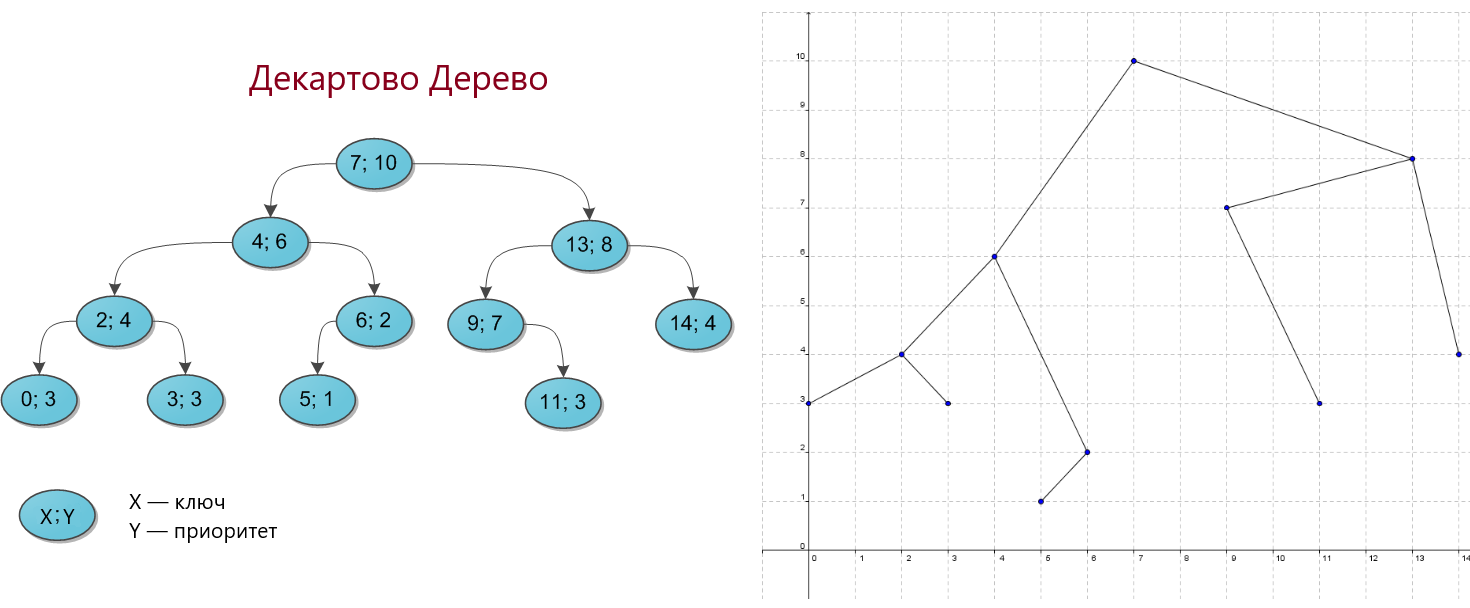
\includegraphics[scale=0.45]{img/treap.png}

Теперь перейдём к работе с Декартовым деревом (ДД), которое поддерживает достаточно много операций: добавление элементов, их поиск и удаление (по ключам). Кроме того, ДД может разбиваться на два других ДД по определённому ключу и также сопоставлять индексу элемента его значение и наоборот. Отсюда видно, что ДД объединяет в себе функционал массивов (получение элемента по индексу), множеств (поиск элементов) и куч (ДД является кучей по приоритетам), то есть такая структура может очень даже пригодиться.

При этом, так же, как и в куче, через две операции (разбиения и слияния) можно выразить все другие операции. Но перед этим стоит сказать, что в нашей реализации ДД в каждой вершине будут храниться: ключ, значение и \term{указатели} на левое и правое поддеревья. Про указатели нужно знать то, что это не сами данные, а лишь информация о месте их расположения. что позволит нам переходить от родительской вершины к дочерним. Кроме того, хранить всё ДД мы будем с помощью её корня.

Начнём с операции разбиения ДД по ключу $key$. Разбивать мы будем рекурсивно, начиная с корня, а получить мы хотим два ДД таких, что в левом все ключи меньше, чем $key$, а в правом — все остальные. Пусть мы сейчас находимся в какой-то вершинке и требуется разбить ДД, за которое она отвечает. Тогда по ключу в вершине мы можем понять, куда она пойдёт: 

\begin{itemize}
    \item Если ключ в вершине больше (или равен) $key$, то это значит, что вершина вместе со своим правым ребёнком должны оказаться в правом поддереве (так как по ключам у нас дерево поиска). То есть остаётся лишь рекурсивно разбить левую часть, и, очевидно, присоединить средний кусок из трёх к правому.
    \item Аналогично при ключе в вершине меньшим $key$ разбивать придётся правое поддерево. А из трёх образовавшихся частей две левых имеют ключи меньшие, чем $key$, поэтому из нужно объединить.
\end{itemize}

Операция слияния должна принимать два ДД и объединять их в одно. При этом у первого ДД все ключи должны быть меньше всех ключей второго ДД. А раз по ключам у нас всё определено, то остаётся лишь не нарушить приоритеты. Но здесь всё совсем просто: у одного из ДД в корне приоритет будет больше, чем у другого (пусть у первого, аналогично будет для второго), а поскольку в корне у нас самый большой приоритет, то после объединения корнем станет корень первого ДД. Но тогда мы точно знаем, что в левом поддереве ничего поменяться не может (из-за условия на ключи), а значит в правом поддереве нам нужно будет объединить правого сына первого ДД и второе ДД, что делается рекурсивно.

Две сложных операции мы разобрали, теперь остались операции попроще. Чтобы найти ключ, мы будем пользоваться отсортированностью ключей, и в зависимости от ключа в родителе, выбирать левого или правого сына. А для них поиск можно сделать рекурсивно.

Удаление элемента $key$ мы можем сделать через два разреза: сначала разрежем левее $key$ (в нашей реализации это разбиение по $key$), а после этого правую часть разделим правее $key$ (то есть сделаем разбиение по $key + 1$). Из полученных трёх частей в средней ключи равны $key$ и эту часть нужно удалить. Оставшиеся же части просто соединяем операцией слияния.

И последняя операция — это добавление. Во-первых, мы не хотим хранить повторяющиеся ключи, поэтому если добавляемый ключ уже есть, то ничего делать не будем. Иначе же, мы можем разрезать по этому ключу и объединить три ДД в одно: левое, сам элемент и правое.

Хоть описание получилось достаточно длинным, но в коде это выглядит коротко и лаконично.

\cpp{ds-3}{54}

Но реализация ДД — это хорошо, но ещё бы уметь её пользоваться. Поэтому приведём ещё и примеры работы с полученным ДД:

\cpp{ds-3}{7}

И ещё один нюанс — это функция \lcpp{random} в восьмой строке. Если приоритеты мы получаем из задачи, то эта функция нам не нужна, а если приоритетов нам никто не дал, то придётся генерировать их самостоятельно. За это и отвечает функция \lcpp{random}, которую нужно заменить на понравившийся способ генерировать случайные числа (о них написано в разделе \hyperlink{built-in function}{встроенные функции}).

Теперь немного поговорим, зачем нам нужна такая сложная структура данных, которая хранит кроме ключей ещё какие-то приоритеты. Если бы у нас не было приоритетов, то ключи должны были бы храниться в отсортированном порядке. Но если ключи бы добавлялись в отсортированном порядке, то вместо равномерной древовидной структуры получился бы \term{бамбук} (у каждой вершины. кроме последней, ровно один ребёнок). Тогда каждая операция с таким деревом поиска могла бы выполняться за \O{n}, что долго (потому что такая же сложность операций с массивом).

Но когда мы используем приоритеты, то получается сбалансированная структура, в которой количество уровней составляет \O{\log n}. Но ведь наши рекурсивные функции делают постоянное количество операций на одном уровне, а значит все они работают за \O{\log n}.

Но раньше было заявлено, что ДД — это очень мощная структура данных, а пока наше ДД умеет делать только операции, которые и так уже реализованы в \lcpp{set}. Но, это легко исправить, если научиться искать $k$-й элемент по ключам (или же по указателю на элемент получать его индекс). Этого не умеют обычные множества, но мы легко это можем добавить.

Для этого в каждой вершине будем дополнительно хранить количество вершин в её поддереве. Тогда чтобы узнать $k$-ый элемент мы пойдём от корня и сможем определять, в какую из дочерних вершин спуститься (как мы это делали в ДО). Аналогично узнаётся и индекс элемента. А чтобы размеры поддеревьев хранились правильно, достаточно в конце каждой функции, меняющие ДД, пересчитывать размеры поддерева. Таким образом мы сможем узнавать $k$-ый элемент за \O{\log n}.

Но и это ещё не всё, ведь существуют \term{неявные Декартовы деревья}. Неявные ДД — это ДД, которые хранят в себе массивы: приоритетом элемента является его значение, а ключом — индекс в массиве. Но ДД не зря называется неявным: мы не будем хранить ключи, потому что можем вычислять их во время спуска от корня. Вот так неожиданно получилось, что отказ от приоритетов вреден, а отказ от ключей полезен.

Чтобы вычислять ключи мы будем использовать уже описанную выше технику хранения размера поддеревьев. А поскольку индекс элемента в массиве равен количеству элементов, стоящих раньше искомого, то на каждом спуске к правому сыну мы будем прибавлять размер левого плюс один (размер родителя), а если будем спускаться к левому сыну, то добавлять ничего не будем.

Слияние в неявном ДД останется таким же, как и в явном (потому что там нигде не используются ключи). А вот функция разбиения теперь должна будет вычислять \lcpp{t -> key} перед её использованием согласно описанию выше: это размер левого поддерева плюс количество уже обработанных вершин (будем передавать его рекурсивно ещё одним параметром), или же просто размер левого поддерева, но тогда при переходе в правого сына нужно будет уменьшать $key$, который мы ищем (мы так уже делали в ДО). Таким же образом нужно обработать и \lcpp{t -> key} в функции поиска.

Поскольку мы определяли удаление и добавление элементов через слияния и разбиения, то наши производные функции продолжат работать. Поменяется лишь смысл $key$, которые они принимают: теперь это будет индекс, откуда нужно удалить или куда требуется вставить элемент.

Таким образом у нас получился аналог массива, который за \O{\log n} позволяет делать все операции с собой: добавление, поиск и удаление элементов. Но неявное ДД способно на большее.

Вспомним, что в ДО у нас было вычисление функций на диапазонах и их изменение. Оказывается, что и это умеет ДО, если будет хранить в себе дополнительную информацию.

Например, чтобы вычислить сумму на отрезке нам будет достаточно сохранить в каждой вершине сумму ей поддерева (эту сумму нужно обновлять, когда меняется поддерево). А когда для ответа на сам запрос, мы вырежем нужный кусок массива и в его корне будет храниться сумма на этом отрезке. После этого нужно не забыть восстановить ДД обратно.

А если нам потребует, например, прибавлять на отрезках. то мы дополнительно в вершинах будем хранить сумму прибавлений. Когда будет поступать запрос на обновление, то мы вырежем наш отрезок и в корне отрезка увеличим прибавление. После этого нам нужно будет вновь объединить все три части. Но теперь стоит немного поменять функции объединения и слияния, добавив в них проталкивание. Проталкивание мы запускаем от корневых вершин, меняем значение в корне и помечаем, что в дочерних вершинах нужно сделать обновления. А после этого операции слияния и объединения делаются без потери информации.

А теперь осознаем мощь ДД, пройдя операции, которое не умеет делать ДО. Во-первых, ДО не умеет себя разрезать на части и склеивать ДО из частей. А значит, что если нам, например, требуется сдвигать все элементы массива, то мы можем сделать это очень легко, с помощью стандартных операций ДД.

Также заметим, что ДД может даже разворачивать отрезки массива, если рассмотреть разворот, как операцию на изменения отрезка, а в момент проталкивания менять местами детей. Удивительная операция!

Вот мы и познакомились с ДД, которое умеет делать все операции массивов, множеств и ДО за \O{\log n}, а кроме того, умеет делать и специфичные операции. Также стоит сказать, что существует разреженное ДО, которое по своей сути напоминает неявное ДД.

      % 14    Структуры данных, часть 3
\newpage
\head{Введение в графы}
Сегодня мы начинаем изучение задач, связанных с графами. Таких задач довольно много (как и алгоритмов на графах), поэтому начнём мы с определений, которые нам потом понадобятся, и способов представления графа в памяти компьютера.


\subhead{Определения}
\begin{itemize}
    \item Основные объекты:
    \begin{enumerate}
        \item Вершина — изображается на картинках, как точка, для удобства нумеруется. Множество всех вершин обозначается $V$ (от \term{vertex}), количество вершин обозначается как $n = |V|$.
        \item Ребро — связь между вершинами, чаще всего двумя (хотя есть и обобщения, например, рёбра соединяют по три вершины); задаётся ребро номерами вершин, которые соединяет. Множество всех рёбер обозначается $E$ (от \term{edge}), количество рёбер обозначается как $m = |E|$.
        \item Граф — совокупность вершин и рёбер: $G(V, E)$.
    \end{enumerate}
    \item Ориентированность:
    \begin{enumerate}
        \item Ориентированный — граф, у которого на рёбрах есть направления (т.е по ребру $e = (u, v)$ из $u$ можно пройти в $v$, а из $v$ в $u$ — нельзя).
        \item Неориентированный — граф, в котором у рёбер нет направлений.
        \item Смешанный — граф, в котором у части рёбер есть направления, а у части — нет.
    \end{enumerate}
    \item Свойства вершин:
    \begin{enumerate}
        \item Степень — количество рёбер вершины.
        \item Входящая и исходящая степени — количество входящих и исходящих рёбер для данной вершины ориентированного графа.
        \item Изолированная вершина — вершина со степенью $0$.
        \item Висячая вершина (или лист) — вершина со степенью $1$.
    \end{enumerate}
    \item Свойства рёбер:
    \begin{enumerate}
        \item Путь — последовательность вершин, в которой каждая следующая вершина (кроме первой) соединена ребром с предыдущей.
        \item Цикл — путь, у которого начальная и конечная вершина совпадают.
        \item Простые путь и цикл — те, в которых рёбра не повторяются.
        \item Петля — ребро, соединяющее вершину саму с собой.
        \item Кратные рёбра — рёбра, соединяющие одинаковые вершины.
    \end{enumerate}
    \item Связность:
    \begin{enumerate}
        \item Компонента связности — подграф, в котором между каждой парой вершин есть путь, без учёта направления рёбер.
        \item Компонента сильной связности — то же, что и обычная компонента связности, но с учётом направления рёбер.
        \item Связный граф — граф с одной компонентой связности.
        \item Несвязный граф — граф, в котором больше одной компоненты связности.
    \end{enumerate}
    \item Другие свойства графа:
    \begin{enumerate}
        \item Взвешенный граф — граф, в котором у рёбер есть числа (веса).
        \item Простой граф — граф без петель и кратных ребер.
        \item Дерево — связный простой граф без циклов.
        \item Лес — граф, в котором каждая компонента является деревом.
        \item Полный граф — простой граф, в котором между всеми парами вершин есть ребро.
        \item $k$-дольный граф — граф, вершины которого можно раскрасить в $k$ цветов так, чтобы не было рёбер между вершинами одного цвета (так называемая правильная раскраска).
        \item Неявный граф — граф, в котором рёбра заданы не в явном виде, а через правило. Например, ходы коня на шахматной доске задают такой граф (в этом случаем мы проводим ребро, по правилу \term{ребро $(u, v)$ есть, если конь может походить из клетки $u$ в клетку $v$}).
        \item Остовное дерево — множество всех вершин и подмножество рёбер, которые образует дерево. Его всегда можно выделить в связном графе, в несвязном есть остовный лес — остовное дерево для каждой компоненты связности.
    \end{enumerate}
\end{itemize}


\subhead{Представление в информатике}
Если мы работаем с неориентированным графом, то каждое ребро $(u, v)$ можно хранить два раза: отдельно для вершины $u$ и отдельно для $v$. Если граф ориентирован, то таких проблем не возникает и каждое ребро можно хранить ровно один раз. В смешанных графах, которые не встречаются в олимпиадном программировании, можно заменить неориентированные рёбра на пару ориентированных.

Если мы работаем со взвешенным графом, то если ребро есть, то мы будем хранить его вес; если же ребра нет, то можно хранить какое-то специальное значение ($0$, $-\infty$ или $+\infty$ в зависимости от задачи), или не хранить ребро вовсе. Если же граф невзвешенный, то можем считать вес каждого ребра равным $1$, что будет просто обозначать наличие ребра.

Теперь мы рассмотрим основные способы представления взвешенного ориентированного графа.

\begin{itemize}
    \item \textbf{Матрица смежности.} Таблица размера $n \times n$, в которой в строке $i$, столбце $j$ мы храним вес ребра из $i$ в $j$. Недостатки — большой расход памяти \O{n^2} и невозможность хранить кратные рёбра.
    \item \textbf{Список смежности.} Для каждой вершины $u$ сохраним список вершин $v$, в которые можно попасть из $u$. Достоинства — легко обойти граф (получить вершины, в которые можно пойти из текущей), малый расход памяти \O{n + m}.
    \item \textbf{Список рёбер.} Просто сохраним информацию о каждом ребре (соединяемые вершины, вес, ориентированность). Достоинство — малый расход памяти \O{m}, из-за чего чаще всего именно так и дают граф во входных данных.
\end{itemize}

Эти способы представления графа легко запомнить, если думать о количестве вершин каждого ребра, которые мы хотим сохранить как дополнительную информацию (0. 1 и 2 соответственно для способов выше).
      % 15    Введение в графы
\newpage
\head{Обходы графа}
Раз уж мы научились хранить графы в памяти компьютера, то можем и начать изучать алгоритмы на графах. Начнём мы с самых простых — обхода графа, потом научимся работать с компонентами связности, потом изучим ещё одну сортировку — топологическую (только это сортировка не обычного набора, а вершин графа). И в самом конце нас ждут компоненты сильной связности, мосты и точки сочленения.


\subhead{Поиск в ширину}
Первый алгоритм обхода это \term{BFS} (от \term{Breadth First Search} — обход графа в ширину. Этот алгоритм начинает обходить граф со стартовой вершины, потом посещает её соседей, потом соседей её соседей, и так далее, слой за слоем, пока соседи не закончатся. 

BFS основывается на очереди $q$ из вершин, которые ещё нужно посетить и списке $used$, хранящим информацию, какие вершины уже добавлялись в очередь (чтобы не обходить их два раза). Для этого сначала в $q$ добавляется стартовая вершина $s$ и она отмечается в $used$. Далее алгоритм шаг за шагом делает следующие операции:

\begin{enumerate}
    \item Берёт первую вершину $u$ из $q$ и удаляет её из $q$.
    \item Обходит все вершины $v$, связанные ребром с $u$. Если очередная вершина $v$ помечена в $used$, то пропускаем ей; если же в вершине $v$ мы ещё не бывали, то добавляем её в конец $q$ и отмечаем её в $used$.
    \item Если в $q$ ещё остались вершины, то операции нужно повторить.
\end{enumerate}

Благодаря списку $used$ каждая вершина добавляется в $q$ ровно один раз, а значит, на каждое ребро мы смотрим не более двух раз (потому что у ребра два конца), следовательно, сложность такого алгоритма будет \O{n + m}. Но, такая сложность доступна, только если граф представлен списком смежности, ведь только такое представление (из изученных) позволяет быстро получать всех соседей вершины.

Также понятно, что такой алгоритм применим на любом графе (ориентированном, взвешенном, не связном, не простом и т.д.) и при этом обходит все достижимые вершины, в частности, для неориентированных графов такой алгоритм посетит всю компоненту связности (для ориентированных тоже можно, если не учитывать направление рёбер, но это менее полезно).


\subhead{Поиск в глубину}
Второй алгоритм обхода это \term{DFS} (от \term{Depth First Search} — обход графа в глубину. Этот алгоритм начинает со стартовой вершины, потом посещает её первого соседа, потом первого соседа первого соседа, и так далее, пока остаются вершины, потом возвращается на несколько вершин, посещает второго соседа и так далее.

DFS основывается на рекурсии и списке $used$, хранящем информацию о том, какие вершины уже посещались. Для этого запускаем рекурсивный алгоритм, начиная со стартовой вершины $s$, и далее действуем шаг за шагом:

\begin{enumerate}
    \item Пусть мы запустились от вершины $u$, тогда её нужно отметить в $used$ как посещённую.
    \item Теперь обойдём все вершины $v$, в которые ведут рёбра из $u$. Если очередная вершина $v$ уже отмечена в $used$, то пропускаем эту вершины; иначе запускаем рекурсивный алгоритм от этой вершины $v$.
\end{enumerate}

Благодаря списку $used$ обход от каждой вершины запускается ровно один раз, а значит на каждое ребро мы смотрим не более двух раз (потому что у ребра два конца), и итоговая сложность алгоритма будет \O{n + m}. При этом DFS, также как и BFS, требует быстро получать соседей очередной вершины, а значит такая сложность достигается только на списках смежности.

При этом этот обход работает на любом графе и, как и предыдущий, посещает все достижимые вершины, а значит для неориентированных графов он посетит всю компоненту связности (можно искать их и в ориентированных графах, если не учитывать направление рёбер, но это мало полезно).


\subhead{Компоненты связности}
Как мы заметили, оба обхода графа (в ширину и в глубину) из заданной вершины $s$ посещают всю компоненту связности. А значит их можно модифицировать, чтобы найти все компоненты связности (и их свойства).

Запустим цикл, перебирающий все вершины. Если очередная вершина $s$ уже посещалась обходом, то пропускаем её; иначе запускаем какой-нибудь обход от этой вершины $s$. При этом можно сделать три (или больше) полезных модификации алгоритма:

\begin{enumerate}
    \item Считать количество запусков обхода, это и будет количеством компонент связности.
    \item Если во время каждого обхода считать количество посещаемых вершин, то получим размер компонент связности.
    \item С помощью $used$ можно определить к какой компоненте связности относится какая вершина. Для этого при первом запуске обхода посещаемые вершины в $used$ помечаем числом $1$, при втором обходе — числом $2$, и так далее (при этом непосещённые вершины отмечены, например, как $0$).
\end{enumerate}


\subhead{Топологическая сортировка}
Пусть у нас есть ациклический (без циклов) ориентированный граф, в котором нужно упорядочить вершины так, чтобы рёбра шли только слева направо (представим, что все вершины записаны в одну строчку). Для этого мы можем использовать уже изученные нами обходы графа (следовательно граф должен быть представлен как список смежности), которые сформируют список вершин $ts$ в порядке топологической сортировке. 

\textbf{Алгоритм Кана}, он же модификация BFS и основывается на очереди $q$. Сначала посчитаем для каждой вершины $deg\_in_i$ — входящую степень вершины $i$ и все вершины с $deg\_in_i = 0$ добавим в очередь $q$. Далее будем действовать следующим образом:

\begin{enumerate}
    \item Берём первую вершину $u$ из $q$ и удаляет её из $q$. Добавляем $u$ в список $ts$.
    \item Проходим по всем рёбрам $(u, v)$ (из вершины $u$ в вершину $v$). Уменьшаем входящую степень $deg\_in_v$ на 1 и если оказалось, что $deg\_in_v = 0$, то добавим $v$ в $q$.
    \item Повторяем эти операции, пока в $q$ остаются вершины.
\end{enumerate}

Теперь осознаем, почему этот алгоритм корректен. Понятно, что если у вершины $deg\_in_i = 0$, то в вершину $i$ не входят рёбра, а значит ей вполне можно поставить самой первой из всех оставшихся (если какие-то рёбра входили в $i$, то их начала уже были добавлены в $ts$, а значит всё на этой вершине правильно). Остаётся понять, что вершина с нулевой входящей степенью всегда должна быть: понятно, что такая вершина должна быть в начале, ведь иначе нет вершины, которая бы стала первой; также понятно, что это должно выполняться на каждом шаге, ведь мы удаляем вершины со всеми выходящими рёбрами, а значит остаётся только подграф, который тоже должен топологически сортироваться (ведь иначе и весь граф не отсортируется). То есть мы выяснили, что наш алгоритм корректен.

Сложность у этого алгоритма такая же \O{n + m}, как и предыдущих, ведь он добавляет каждую вершину в $q$ ровно один раз, а значит и на каждое ребро смотрит только один раз (т.к. граф ориентирован, то мы смотрим только с одной стороны, откуда ребро выходит).

\textbf{Алгоритм Тарьяна}, он же модификация DFS. Единственная модификация заключается в том, что в конце рекурсивной функции для вершины $u$ нужно будет добавить $u$ в конец $ts$. А когда все компоненты связности будут обработаны, то нужно будет развернуть $ts$.

Понятно, почему такой алгоритм работает, ведь когда мы заканчиваем рекурсивную функцию для вершины $u$, то это значит, что мы обработали уже все вершины, достижимые из $u$ и добавили их в $ts$, а значит после добавления вершины $u$ в $ts$ получим, что все рёбра из $u$ идут влево, поэтому в конце мы и разворачиваем $ts$.

Также понятно, что сложность у этого алгоритма \O{n + m} такая же, как и у DFS, ведь их разница только в формировании списка $ts$, что делается быстро за \O{n}.


\subhead{Компоненты сильной связности}
Пусть нам дан ориентированный граф, в котором требуется найти компоненты сильной связности (КСС, или SCC от \term{Strongly Connected Component}). Оказывается, что для решения такой задачи достаточно всего лишь модифицировать DFS.

\textbf{Алгоритм Косараджу}, основанный на двух DFS:

\begin{enumerate}
    \item Запустим обычный DFS, который запишет вершины в порядке выхода алгоритма из них (как $ts$ в Алгоритме Тарьяна для топологической сортировки), назовём этот список $tout$.
    \item Теперь будем рассматривать транспонированный граф (у него все рёбра развёрнуты относительно исходного графа).
    \item Будем запускать второй DFS от вершин в порядке уменьшения $tout$ для них. Все вершины, которые посещаются одним таким обходом являются одной SCC (посещается вся компонента и при этом без других вершин).
\end{enumerate}

Алгоритм выглядит понятным, но вот его корректность не очевидна, поэтому будем её доказывать. Во-первых нужно понять, что в обоих графах (исходном и транспонированном) SCC одинаковые (в самом деле, пусть $u$ и $v$ лежат в одной SCC в исходном графе, тогда есть какие-то пути $a: u \to v$ и $b: v \to u$, но после транспонирования они превратятся в $a^T: v \to u$ и $b^T: u \to v$, а значит $u$ и $v$ снова будут лежать в одной SCC; аналогично вершины разных SCC попали в разные SCC).

Для этого рассмотрим две компоненты сильной связности $C_1$ и $C_2$, между которыми есть путь из $C_1$ в $C_2$ (если бы при этом было путь из $C_2$ в $C_1$, то компоненты бы объединились в одну; если же между компонентами нет пути, то алгоритм, очевидно, работает). Рассмотрим вершину $u$, которая является первой из посещённых в $C_1$ и $C_2$ первым DFS.

Пусть $u$ лежит в $C_1$, тогда после этого он в каком-то порядке посетил остальные вершины из $C_1$ и из $C_2$ и потом вышел из них. Следовательно алгоритм сначала вышел из всех вершин $C_2$ и только потом вернулся в $u$ и вышел из неё. Но тогда запуск второго DFS сначала произойдёт из $u$, и попасть в $C_2$ мы не сможет (ведь второй DFS запускается на транспонированном графе), то есть в таком случае наш алгоритм работает корректно.

Иначе $u$ лежит в $C_2$. тогда сначала посетится вся $C_2$ и, возможно, какие-то ещё вершины, но в $C_1$ мы попасть не сможем, ведь туда нет пути. Следовательно мы сначала выйдем из $C_2$ и только потом зайдём и выйдем в $C_1$. То есть также, как и в предыдущий раз, второй DFS сначала запустится в $C_1$ и только потом из $C_2$, а значит и в таком случае всё сработает.

Таким образом мы доказали корректность алгоритма, его сложность понятна, ведь это всего лишь два DFS и транспонирование графа, а такие операции делаются суммарно за \O{n + m}.

\textbf{Алгоритм Тарьяна}, для него хватает одного DFS. Дополнительно нам понадобится в ходе алгоритма поддерживать $tin_i$ — время входа DFS'а в вершину $i$, $fup_i$ — минимальное время ($tin_u$), в которое можно попасть, выйдя из вершины $i$, и $processed_i$ — обозначающая, нашлась ли для $i$ SCC. Ещё мы будем запоминать в стек $s$ текущие вершины, которые ещё не попали ни в одну SCC. Изначально считаем все $tin_i = fup_i = -1$, $processed_i = false$, $s$ — пуста.

\begin{enumerate}
    \item В начале обхода вершины $u$ нужно: добавить $u$ в $s$, отметить её, как вычисляющуюся $processed_u = true$ и присвоить в $tin_u = fup_u$ текущее значение таймера (и увеличить таймер на 1).
    \item Перебираем все рёбра $u \to v$. Если очередную вершину $v$ мы ещё не посещали ($tin_v = -1$), то для неё нужно запустить DFS. После этого, если $processed_v = true$, то следует обновить $fup_u = \min(fup_u, fup_v)$.
    \item Если после обработки всех рёбер $u \to v$ значение $fup_u$ не обновилось ($fup_u = tin_u$), то это значит, что текущая вершина является началом SCC. Поэтому будем снимать вершины $x$ со стека, отмечать их как обработанные ($processed_x = false$) и добавлять к текущей SCC. Если же оказалось, что $x = u$, то SCC закончилась и можно выходить из функции.
\end{enumerate}

Понятно, почему такой алгоритм работает, ведь SCC должны образовывать циклы, а цикл обязательно заканчивается где-то в вершине $a$ среди обрабатывающихся вершин. А раз так, то дойдя до $a$ мы начнём постепенно возвращаться к предыдущим вершинам $b$ цикла и по сути делать для них обновление $fup_b = \min(fup_b, tin_a)$, в вершине $a$ такое обновление ничего не даст, поэтому мы найдём начало цикла (если же из $a$ есть ещё какие-то рёбра в более ранние вершины, то после их посещения $fup_a$ уменьшится и мы цикл на этом шаге не найдём, ведь его начало было где-то ещё раньше).

Также понятна временная сложность алгоритма \O{n + m}, потому что мы всего лишь модифицировали DFS, при этом все новые операции выполняются за постоянное время.


\subhead{Мосты и точки сочленения}
Пусть нам дан неориентированный граф, и в нём требуется найти \term{мосты} — рёбра, после удаления которых число компонент связности увеличивается и \term{точки сочленения} — вершины, после удаления которых компонент связности становится больше. Как это ни удивительно, но и для этого нам достаточно всего лишь модифицировать DFS.

Но перед быстрым алгоритмом заметим, что относительно легко можно придумать медленный алгоритм, который сначала запускает DFS, считающий компоненты связности, а потом по очереди убирает все вершины и рёбра и проверяет, сколько компонент стало. Но такой алгоритм действительно долгий, со сложностью \O{(n + m)^2}, а нам хотелось бы быстрее.

Давайте снова будем вычислять $tin_i$ — время входа DFS'а в вершину $i$, $fup_i$ — минимальное время ($tin_u$), в которое можно попасть, выйдя из вершины $i$. Изначально считаем все $tin_i = fup_i = -1$. После этого запускаем обход от вершины $root$.

\begin{enumerate}
    \item Пусть обход перешёл в вершину $u$ из вершины $p$ (для $root$ считаем, что $p = -1$). И присваиваем $tin_u = fup_u$ текущее значение таймера (и увеличить таймер на 1).
     \item Перебираем все рёбра $(u, v)$. Если $v = p$, то такое ребро нужно пропустить. Если очередную вершину $v$ мы уже посещали ($tin_v > -1$), то нужно обновить $fup_u = \min(fup_u, tin_v)$.
     \item Если же $v$ мы ещё не посещалась, то нужно запустить для неё DFS (передав $u$ как родительскую вершину) и обновить $fup_u = \min (fup_u, fup_v)$. Если $u = root$, то нужно запомнить, что запускался DFS, иначе если $fup_v \geq tin_u$, то из $v$ не нашёлся путь куда-то вверх, а значит $v$ — точка сочленения, а если $fup_v > tin_u$, то ребро $(u, v)$ является мостом.
     \item Если после обхода всех рёбер оказалось, что $u = root$ и мы запускали DFS больше одного раза, то посещённые поддеревья не связаны, а значит, $root$ — точка сочленения.
\end{enumerate}

Понятно, что такой алгоритм работает, ведь, $fup_i$ действительно подсчитывает наименьшее время, достижимое из $i$, а критерии моста $fup_v > tin_u$ и точки сочленения $fup_v \geq tin_u$ понятны, ведь это и обозначает, нашёлся ли путь в какую-то более раннюю вершину. Наличие отдельного критерия для $root$ тоже понятно, ведь корневая вершина никогда не попадает под обычное условие, так как время входа в неё минимальное.

Сложность этого алгоритма (как и всех предыдущих алгоритмов обхода) составляет \O{n + m}, что явно лучше нашего тривиального решения.
      % 16    Обходы графа
\newpage
\head{Остовные деревья и кратчайшие пути}
Мы продолжаем изучать графы, и сегодня займёмся поиском \term{минимального остовного дерева} — остовного дерева в неориентированном графе с минимальным суммарным весом рёбер, и модификациями данной задачи, а после этого будем искать \term{кратчайшие пути} между парой вершин, от одной вершины до всех остальных и между всеми парами вершин. Хоть алгоритмов и много, но все они (почти) достаточно понятны и частично основываются на уже пройденных алгоритмах.


\subhead{Минимальное остовное дерево}
На самом деле, раньше мы уже находили остовные деревья, когда совершали обходы графа (для DFS это дерева строится рекурсией, а для BFS дерево создаётся из рёбер, помещающих новые вершины в очередь). Поэтому если наш граф невзвешенный, то мы можем считать все веса рёбер равными 1, а значит любое остовное дерево будет являться минимальным, то есть мы уже частично умеем решать задачу. Но для взвешенных графов алгоритм не такой простой, поэтому перейдём к его изучению.

\textbf{Алгоритм Прима.} Это своего рода модификация алгоритмов обхода графа, потому что запустимся мы от одной вершины и рёбра будем добавлять последовательно (так, что всё время будем иметь дерево). Также нам понадобится знать, какие вершины уже в дереве (список $used$) и структура данных, позволяющая быстро выбирать минимальный элемент (множество / отображение или куча), назовём её $p$. И алгоритм выглядит так:

\begin{enumerate}
    \item Произвольно выберем стартовую вершину $u$, пометим её в $used$ и добавим все рёбра $(u, v)$ в $p$, при этом $p$ должна уметь выдавать ребро с минимальным весом.
    \item Теперь пока структура $p$ не пуста будем брать из неё минимальное ребро $(u, v)$ и удалять его из $p$. Если так оказалось, что обе вершины ($u$ и $v$) уже в дереве (помечены как $used$), то ребро нужно пропустить. А иначе мы добавляем ребро $(u, v)$ в итоговое дерево, помечаем $v$ как $used$ ($u$ уже в дереве, потому что ребро оказалось в $p$) и добавляем в $p$ все рёбра $(v, t)$, где $t$ ещё не в дереве (не $used$), чтобы избежать зацикливания.
\end{enumerate}

Понятно, почему такой алгоритм работает, ведь из уже существующего минимального дерева какое-то ребро провести придётся и поэтому мы выбираем максимальное. А раз мы так делаем пока все доступные рёбра не получатся, то мы как раз получим минимальное остовное дерево текущей компоненты связности. Если же ещё есть другие КС, то будем запускать построение дерева от каких-то вершины из них и в итоге получим минимальный остовный лес.

Чем полезен такой алгоритм, так это возможностью смотреть не на все рёбра, а только на их часть, при выборе следующего ребра. Также для этого алгоритма граф должен быть представлен как список смежности, что тоже удобно, потому он применим в большом количестве других задач. 

Сложность такого алгоритма составляет \O{m \log m}, так обрабатывается $m$ рёбер и на каждое из них тратится \O{\log m}, ведь его нужно добавить в $p$ и достать из неё, а делается это не быстрее, чем за логарифм размера $p$. Также можно улучшить алгоритм до \O{m \log n}, если для каждой вершины хранить только минимальное ребро, ведущее в неё, но даже если считать, что в графе много рёбер, то $m = O(n^2)$ и $O(m \log m) = O(m \log n^2) = O(2m \log n) = O(m \log n)$, поэтому фактически улучшение может и не быть.

\textbf{Алгоритм Краскала.} Этот алгоритм сильно отличается от предыдущего, но схож тем, что на очередном шаге выбирает минимальное ребро. Для алгоритма нам понадобится список рёбер $e$, список $used$ посещённых вершин и структура $p$, позволяющая объединять множества и проверять элементы на принадлежность одному множеству (в простейшем случае можно использовать массив, но с DSU будет быстрее):

\begin{enumerate}
    \item Для начала отсортируем $e$ по неубыванию веса, а в структуре $p$ размера $n$ сохраним, что все вершины пока принадлежат разным множествам (деревьям).
    \item Теперь будем перебирать все рёбра от меньшего веса к большему и если очередное ребро $(u, v)$ соединяет разные деревья, то это ребро нужно добавить к итоговому дереву и в $p$ объединить множества, представленные $u$ и $v$.
\end{enumerate}

Понятно, что и этот алгоритм тоже работает, ведь когда мы добавляем ребро $(u, v)$, то соединяем множество вершины $u$ с остальным деревом, и делаем мы это ребром с минимальным доступным весом. А значит и получаем в конце минимальное остовное дерево для связного графа и минимальный остовный лес для несвязного графа.

Сложность же алгоритма также составляет \O{m \log n}, ведь нам требуется $O(m \log m) = O(m \log n^2) = O(2m \log n) = O(m \log n)$ на сортировку рёбер и после этого мы выполняем \O{m} операций с $p$, которые в DSU можно реализовать за \O{\ac{n}}, то есть итого имеем $O(m \log n + m \ac{n}) = O(m \log n)$. Также важно, что этому алгоритму, в отличие от предыдущего, требуется список рёбер, что может быть несколько не удобно, но в зато этот алгоритм будет легко модифицировать, что мы дальше и увидим.


\subhead{Модификации минимального остова}
Искать только минимальное остовное дерево — это скучно, поэтому существуют другие схожие задачи, которые решаются теме же алгоритмами, что мы и прошли, после внесения небольших изменений. При этом нам будет проще вносить изменения в алгоритм Краскала, но некоторые задачи также решаемы и с помощью алгоритма Прима. Рассмотрением этих задач мы и займёмся.

\textbf{Максимальное остовное дерево.} В общем-то понятно, что здесь нужно сделать: раз у нас вместо минимума нужно найти максимум, то достаточно поменять правило сортировки на противоположное. То есть, для алгоритма Прима мы будем выбирать ребро с максимальным весом, а для алгоритма Краскала будем идти от рёбер с большим весом к рёбрам с меньшим весом. Но можно поступить более олимпиадно и поменять все веса $w \to -w$ и использовать уже их в обычных алгоритмах :)

\textbf{Минимальное достроение.} Пусть у нас в графе уже выбраны какие-то рёбра и нам нужно ещё выбрать какие-то рёбра так, чтобы суммарный вес был минимальным и количество компонент связности было таким же, как и в исходном графе.

Решить эту задачу также не сложно с помощью алгоритма Краскала. Для этого, перед запуском основного алгоритма, добавим все обязательные рёбра к результату и отметим в $p$, что какие-то множества соединены ребром. А после этого сделаем обычный запуск алгоритма Краскала.

\textbf{Лес из заданного числа компонент связности.} Пусть нам требуется найти минимальный остовный лес, но при этом он должен состоять из $k$ компонент связности (где $k$ не меньше, чем количество исходных КС).

Это тоже достаточно простая задача, ведь алгоритм Краскала на каждом шаге действует жадно, поэтому его достаточно будет прервать, когда останется $k$ компонент связности. Определить же это можно посчитав количество добавленных рёбер, их должно быть $m' = n - k$, ведь в каждой КС рёбер $m'_i = n_i - 1$ (так как это деревья), а всего $n = \sum\limits_{i = 1}^{k} n_i$, а значит $m' = \sum\limits_{i = 1}^{k} m_i = \sum\limits_{i = 1}^{k} (n_i - 1) = \sum\limits_{i = 1}^{k} n_i - k = n - k$. Такую же формулу можно получить, если учесть, что изначально мы имеем $n$ КС, а должны сделать $k$ КС, при этом каждое проводимое ребро объединяет две КС, а значит $m' = n - k$.

\textbf{Минимакс и максимин.} Минимаксом называет поиск пути между вершинами $i$ и $j$ такой, что вес этого пути минимален. При этом весом пути называется максимальной вес ребра, которые встречается на этом пути. Аналогично определяется максимин, там нужно максимизировать минимальный вес ребра на пути.

Если подумать, то оказывается, что искомый путь будет лежать в минимальном остовном дереве. В самом деле, при построении минимального остовного дерева мы на каждом шаге выбираем минимальное ребро, а значит и на пути между $i$ и $j$ добавляется ребро с минимальным возможным весом, а следовательно максимальный вес среди них действительно минимально возможный.

Итоговым алгоритмом будет: сначала найти минимальное остовное дерево, а после этого запустить какой-нибудь обход графа и найти максимальное значение на пути между $i$ и $j$. Итоговая сложность будет такой же, как и у построения дерева, ведь его обход выполняется за линейное время (так как в дереве имеем $m = n - 1$, и алгоритмы обхода отработают за $O(n + m) = O(n + n - 1) = O(n)$).

\textbf{Второе лучшее остовное дерево.} В этой задаче требуется найти не минимальное остовное дерево, а второе по минимальности. Это задача уже не такая очевидная, и сложность у неё получится несколько больше.

Заметим, что второе по минимальности остовное дерево можно получить, если произвести всего одну замену в обычном минимальном остовном дереве (то есть одно ребро удалить и одно добавить). И понятно, почему это условие выполняется, ведь если мы производим замену, то от этого суммарный вес дерева только увеличивается, а если делать несколько таких замен, то вес увеличится ещё больше. Следовательно, второе лучшее дерево отличается от лучшего всего одной заменой.

А раз так, то сначала построим первое лучшее дерево, а потом будем по очереди запрещать использовать его рёбра и строить новые минимальные остовные деревья. Тогда нам потребуется \O{m \log n} на первоначальную сортировку, \O{m} на поиск лучшего оствного дерева и после этого мы будим закрывать \O{n} рёбер, тратя на каждое ещё один поиск лучшего остовного дерева за \O{m}. И итоговая сложность будет \O{nm}. Но стоит отметить, что можно ускорить алгоритм, если использовать DSU или LCA, но это уже остаётся на изучение читателю :)


\subhead{Кратчайшие пути от одной вершины до всех}
С минимальными остовными деревьями мы разобрались, поэтому можем переходить к кратчайшим путям. При этом хотелось бы начать с кратчайшего пути между парой вершин, но для этой задачи нет отдельного алгоритма, поэтому мы начнём с кратчайшего пути из одной вершины во все.

Оказывается, что и эту задачу мы уже умеем решать для невзвешенных графов с помощью BFS. Для этого в BFS будем поддерживать $d_i$ — номер слоя для вершины $i$, который нужно пересчитывать при добавлении вершины $i$ в очередь из-за ребра $x \to i$, как $d_i = d_x + 1$. Но всё же это частный случай для невзвешенных графов, а хочется уметь решать задачу в общем виде, поэтому перейдём к изучению алгоритмов для взвешенных графов.

\textbf{Алгоритм Дейкстры.} Этот алгоритм похож на смесь BFS и алгоритма Прима. И своей целью ставит определение $d_i$ — расстояние от стартовой вершины $s$ до вершины $i$. При этом во время работы алгоритма нам понадобится брать вершину с минимальным расстоянием, и из-за разных способов это сделать мы будем получать разные сложности.

\begin{enumerate}
    \item Положим $d_s = 0$ и $d_u = \infty$\footnote{Здесь и далее константу $\infty$ нужно выбирать так, чтобы сумма $\infty + \infty$ ещё входила в тип данных!}, для $u \ne s$.
    \item Теперь в цикле будем выбирать необработанную вершину $u$ с минимальным расстоянием до ней (как это делать будет описано ниже). Обходим все рёбра $(u; v)$ и пытаемся обновить минимальное расстояние $d_v = \min(d_v, d_u + c)$, где $c$ — это стоимость ребра $(u, v)$.
\end{enumerate}

Собственно, это и есть весь алгоритм, теперь осталось понять, как искать вершину $u$.

Выбирать вершину $u$ можно с помощью массивов. Для этого дополнительно будем поддерживать список $used$, отвечающий за посещённость вершины (будем отмечать вершину $u$ в $used$, до обхода рёбер из $u$). И теперь для выбора минимальной вершины будем проходить по всем вершинам и выбирать ту, у которой $d_i$ минимальна и при этом она ещё не посещалась согласно списку $used$. Заканчивать же алгоритм мы можем или когда посещены все вершины, или когда посещена все КС (тогда мы сможем найти только $d_i = \infty$ среди не посещённых вершин).

Другой способ — это использовать множество / отображение или кучу $p$. Тогда в самом начале нам нужно добавить пару $(0; s)$ в $p$. А после этого на каждом шаге брать минимальную пару $(u, c)$ из $p$ и уже работать с этой вершиной. При этом после изменения расстояния до вершины $v$ нам нужно добавить ей в $p$ (в таком же формате $(v, d_v)$). Но понятно, что так одна и та же вершина $v$ может попасть в $p$ из-за разных вершин $u$, а обрабатывать мы её хотим только один раз. Поэтому если нам позволяет структура данных $p$, то перед добавлением нужно будет удалить старое значение для вершины $v$, что мы и будем делать для встроенных в C++ множеств и отображений, а также для самописной кучи. А если же мы используем встроенную в C++ кучу, то операции удаления в ней нет, поэтому обходить все рёбра из $u$ мы будем только в случае, когда $c = d_u$ (то есть между добавлением пары в кучу и обновлением вершин не было других обновлений). Заканчивать же алгоритм мы в любом случае будем, когда $p$ станет пусто.

Алгоритм, конечно, хороший и понятный, но в общем есть одна проблема — он не всегда работает. Пусть мы уже правильно обработали какое-то множество вершин (нашли кратчайшие пути до них) и все рёбра, выходящие из них, а сейчас обрабатываем вершину $u$. Тогда для неё $d_u$ будет правильным ответом только если нет рёбер отрицательного веса $w$, ведь если они существуют, то может найтись ещё какая-то вершина $x$ такая, что $d_x > d_u$, но при этом $d_x + w < d_u$, а значит для вершину $u$ у нас пока не правильный ответ. Но вот если все веса неотрицательны то точно всё хорошо, ведь тогда для любого $x$ будем иметь $d_x > d_u$ и $d_x + w > d_u$.

Поэтому алгоритм Дейкстры работает только для графов без рёбер отрицательного веса, а его сложность для случая с массивами будет \O{n^2 + m}, потому что мы для каждого шага перебираем все вершины и плюс просматриваем все ребра. А вот если использовать правильные структуры данных, то имеем сложность \O{m \log n}, потому что в худшем случае каждое ребро обновляет кратчайшие пути, а на одну операцию с $p$ требуется $O(\log n)$ операций в случаи с удаление повторов и $O(\log m) = O(\log n^2) = O(2 \log n) = O(\log n)$ если повторы не удалять :) Всего же таких операций $m$ для рёбер 
$n$ для взятия минимальной вершины, поэтому на самом деле сложность составляет \O{(n + m) \log n}.

Также стоит сказать, что есть решение со сложностью \O{n \log n + m}, если использовать \term{Фибоначчиевы кучи}, и линейный алгоритм Торупа, но это тоже остаётся для самостоятельного изучения читателями.

\textbf{Алгоритм Форда–Беллмана.} На самом деле, разобранная выше реализация алгоритма Дейкстры на основе кучи без удаления лишних пар всё же умеет обрабатывать отрицательные веса рёбер (просто работает несколько дольше, потому что делает несколько обновлений для одной вершины), но ломается, если в графе есть цикл отрицательного веса (обновления в алгоритме Дейкстры происходят бесконечно). Именно для этого и нужно использовать очень простой алгоритм Форда–Беллмана, вычисляющий $d_i$ минимальное расстояние от $s$ до $i$:

\begin{enumerate}
    \item Изначально принимаем $d_s = 0$ и $d_u = \infty$, для $u \ne s$.
    \item Теперь повторим цикл $n-1$ раз, в каждом из которых для всех рёбер $(u, v)$ с весом $c$ сделаем \term{релаксацию} (обновление ответа): $d_v = \min(d_v, d_u + c)$. 
\end{enumerate}

И это собственно весь алгоритм!

А если нужно проверить, есть ли цикл отрицательного веса, то достаточно ещё раз сделать релаксацию для всех рёбер и проверить, поменялись ли ответы: если поменялись, то есть цикл отрицательного веса, если нет — то и цикла нет. Просто, правда? :)

Но и в таком простом алгоритме можно сделать пару модификаций. Во-первых, если на каком-то шаге не один $d_i$ не обновился, то у нас уже есть ответ. А во-вторых, если нужно, то можно восстановить сами кратчайшие пути (как, собственно, и в алгоритме Дейкстры).

Теперь быстренько докажем правильность этого алгоритма. Заметим, что на $i$-ой итерации цикла мы получаем правильные ответы для всех вершин, кратчайшие расстояния до которых состоят из $i$ рёбер. Это утверждение очевидно, ведь на первом шаге мы посетим первое ребро и получим оптимальный ответ для первой вершины, на втором шаге точно посмотрим на второе ребро пути и получим ответ для второй вершины, и так далее, а на $i$-ом шаге как раз пройдём по $i$-ому ребро и получим ответ для этой вершины. А поскольку граф состоит из $n$ вершин, то самый длинный путь может состоять из $n - 1$ ребра, именно столько итераций цикла мы и делаем, а значит наш алгоритм корректен.

Также стоит сказать, что граф можно хранить и как список рёбер, и как список смежности, и тогда сложность этого алгоритма \O{n m}, хоть это читатель мог понять и сам :) А вот если мы работаем с матрицей смежности, то на каждом шаге цикла будем проходить всю матрицу и получим сложность \O{n^3}.


\subhead{Кратчайшие пути между всеми парами вершин}
Раз уж мы решали задачу для случая с одной стартовой вершиной, то теперь совсем усложним её и будем искать путь между всеми парами вершин. Наивные решения, которые $n$ раз бы запускали поиск расстояния от одной вершины нас не интересуют, потому что они получатся слишком сложными для $m = O(n^2)$: \O{n^3 \log n} для алгоритма Дейкстры и \O{n^4} для алгоритма Форда–Беллмана, а хочется найти алгоритм быстрее. Поэтому, можно бы начать бояться, что тут будет какой-нибудь очень сложный алгоритм, но на самом деле всё просто:

\begin{enumerate}
    \item Сохраним граф в матрице смежности $g$ и в ячейку $(i, j)$ поставим $\infty$, если в графе нет ребра из $i$ в $j$, а иначе запишем в эту ячейку вес самого ребра. Также считаем, что в вершине можно оставаться: $g_{i \to i} = 0$ (если в графе разрешены петли, то пишем вес петель).
    \item Теперь сделаем цикл $n$ раз и на $k$-ом шаге цикла переберём все пары вершин $(i, j)$ и будем пытаться обновить ответ для этой пары через вершину $k$: $g_{i \to j} = \min(g_{i \to j}, g_{i \to k} + g_{k \to j})$.
\end{enumerate}

Вот и всё, мы получили рабочий алгоритм в 3 цикла и одну операцию!

Давайте докажем этот алгоритм, который основывается на динамическом программировании. Пусть $D_{i \to j}^k$ это оптимальный путь из $i$ в $j$, промежуточно проходящий только через первые $k$ вершин: $1,\ 2,\ \ldots,\ k$. Тогда понятна и основная формула перехода: $D_{i \to j}^{k + 1} = \min( D_{i \to j}^k, D_{i \to k}^k + D_{k \to j}^{k})$, ведь очередная вершина $k$ может как использоваться в пути $i \to j$, так и нет. Базой же динамики будут изначальные кратчайшие расстояния, не проходящие через другие вершины, которые являются весами рёбер: $k = 0$ и $D_{i \to j}^0 = g_{i \to j}$.

Но поскольку в нашей формуле мы вычисляем $D^{k + 1}$ только через $D^k$, то для ответов можно хранить не трёхмерную матрицу $n \times n \times k$, а ограничиться лишь двумя матрицами $n \times n$. А если понять, что от рассмотрения лишних вершин наш ответ не ухудшится, то можно смело хранить ответы для обоих итераций ($k$ и $k + 1$) в одном и том же массиве, именно поэтому мы и имеем такую простую формулу для алгоритма Флойда–Уоршелла (так называется то, что мы прошли).

Понятно, что сложность алгоритма Флойда–Уоршелла составляет \O{n^3}, ведь у нас просто три вложенных цикла. Также понятно, что алгоритму требуется граф, сохранённый в матрице смежности.

В заключение стоит сказать, что можно сделать много модификаций этого алгоритма, которые бы решали разные задачи (но не для больших графов, потому что алгоритм выполнялся бы долго).

Например, можно выводить сами кратчайшие пути, если запомнить, из какой вершины мы попали к текущему ребру: сначала возьмём $p_{i \to j} = i$, и если мы делаем обновление внутри цикла, то сделаем и $p_{i \to j} = p_{k \to j}$, а при выводе пути $i \to j$ нужно будет сначала вывести путь $i \to p_{i \to j}$, а после этого и вершину $j$.

Также можно использовать этот алгоритм для поиска кратчайших путей из одной вершины; для поиска \term{транзитивного замыкания} — проверки, что есть путь $i \to j$; для задач минимакса и максимина; для проверки наличия отрицательного цикла (просто запустим алгоритм ещё раз и все ячейки, в которых поменялись ответы будут иметь ответ $-\infty$). И ещё много других интересных задач, с которыми читатель может ознакомиться сам.
      % 17    Остовные деревья и кратчайшие пути
\newpage
\head{Геометрия: введение}
Сегодня мы начинаем изучение задач, связанных с вычислительной геометрией. Это не обычные геометрические задачи по математике, в которых нужно использовать разные теоремы, чтобы доказать что-то в задаче, а задачи, в которых нужно что-то посчитать. Например, найти площадь, найти точку, уравнение прямой и многое другое.

Сегодня мы рассмотрим такие базовые понятия вычислительной геометрии, как точки (\lcpp{Point}), вектора (\lcpp{Vector}) и прямые (\lcpp{Line}). Всё это мы будем рассматривать на плоскости, потому что задачи про трёхмерное пространство не встречаются. Вычислительная геометрия — это как раз один из тех разделов, в которых на будет очень удобно использовать структуры, поэтому мы научимся работать с ними ещё лучше. Также в вычислительной геометрии очень важна точность, поэтому мы будем использовать шаблоны, чтобы получить реализацию и для целых чисел, и для вещественных.


\subhead{Точки}
Точка очень простой геометрический объект, поэтому каждая точка будет обладать своими координатами (\lcpp{x} и \lcpp{y}), и точки будут поддерживать следующие операции (их достаточно мало):

\begin{itemize}
    \item Создание точки по координатам или без них. Для этого будем использовать конструктор с точкой \p{0}{0} по умолчанию.
    \item Сдвиг точки на вектор. Для этого определим операторы \lcpp{+} и \lcpp{-}, чтобы можно было писать \lcpp{p + v} и \lcpp{p - v}.
    \item Ввод и вывод точки. Определим операторы \lcpp{>>} и \lcpp{<<} с нужными аргументами и C++ сам поймёт, как обрабатывать выражения \lcpp{cin >> p} и \lcpp{cout << p}.
\end{itemize}

Все эти операции можно реализовать следующим образом:

\cpp{geo-1}{11}


\subhead{Вектора}
Хоть вектора, также, как и точки, хранят только два числа (\lcpp{x} и \lcpp{y}), но это уже более сложный объект, поэтому для них нам нужно определить много операций:

\begin{itemize}
    \item Создание вектора по координатам или без них; создание вектора по двум точкам. Для этого будем использовать конструкторы и вектор $\v{(0, 0)}$ по умолчанию.
    \item Сложение и вычитание векторов. Нам помогут бинарные операторы \lcpp{+} и \lcpp{-} чтобы писать \lcpp{v + u} и \lcpp{v - u}, а также их унарные версии, чтобы делать \lcpp{+v} и \lcpp{-v} (как бинарные операции, в которых второй операнд $\v{0}$).
    \item Умножение вектора на число реализуем с помощью операторов \lcpp{*} и \lcpp{/}.
    \item На произведениях векторов нужно остановиться подробнее.
        \begin{enumerate}
            \item \textbf{Скалярное произведение.} В математике обозначается как $\v{v} \cdot \v{u}$ и имеет важное равенство $|v| \cdot |u| \cdot \cos(\widehat{v;u}) = \v{v} \cdot \v{u} = v_x u_x + v_y u_y$. Считать мы, конечно, будем по второй формуле и обозначим такое произведение за \lcpp{v * u}. Также важно знать, что если $\v{v}, \v{u} \ne \v{0}$ и $\v{v} \cdot \v{u} = 0$. то $\v{v} \perp \v{u}$.
            \item \textbf{Псевдоскалярное произведение.} В математике обозначается как $\v{v} \wedge \v{u}$ и имеет важное равенство $|v| \cdot |u| \cdot \sin(\widehat{v;u}) = \v{v} \wedge \v{u} = v_x u_y - v_y u_x$. Считать мы, конечно, будем по второй формуле и обозначим такое произведение за \lcpp{v % u} (потому что хочется, чтобы приоритет произведений был одинаковым, а использовать $/$ как-то странно для произведения). Также важно знать, что если $\v{v}, \v{u} \ne \v{0}$ и $\v{v} \wedge \v{u} = 0$. то $\v{v} \parallel \v{u}$.
        \end{enumerate}
    \item Угол между векторами, обозначается как $\widehat{v;u}$. Понятно, что для этой операции можно придумать формулы через произведения: $\widehat{v;u} = \arccos{ \frac{\v{v} \cdot \v{u}}{|v| \cdot |u|} } = \arcsin{ \frac{\v{v} \wedge \v{u}}{|v| \cdot |u|} }$. Но тогда у нас возникнут дополнительный погрешности при делении (да и нужно бы определить, какой угол между векторами, если знаменатель занулится), поэтому принято считать по формуле $\widehat{v;u} = \arctg{ \frac{\v{v} \wedge \v{u}}{\v{v} \cdot \v{u}} }$. А в программировании есть функция $\atantwo(y, x) = \arctg{\frac{y}{x}}$, которая дополнительно умеет обрабатывать случай $x = 0$. Для угла будем использовать оператор \lcpp{^}, чтобы писать \lcpp{v ^ u}.
    \item Длину вектора мы будем считать по теореме Пифагора: $len = \sqrt{x^2 + y^2}$. При этом в некоторых задачах нам достаточно использовать квадрат длины (например, если мы сравниваем длины векторов), поэтому сделаем отдельную функцию, которая бы не извлекала корень, потому что так вычисления точнее: $sqlen = x^2 + y^2$.
    \item Полярный угол будем считать через $\atantwo(y, x)$.
    \item Используя полярный угол можно легко нормировать вектор, ведь если $\alpha$ — полярный угол вектора $v(x; y)$, то понятно, что $\v{n} = \v{(\cos \alpha; \sin \alpha)}$ будет искомым вектором. Также можно было бы считать по формуле $\v{n} = \v{\left(\frac{x}{|v|}; \frac{y}{|v|}\right)}$.
    \item Перпендикулярным вектором (одним из) для $v(x, y)$ является $u(-y, x)$, так как их перпендикулярность можно проверить через скалярное произведение.
    \item Ввод и вывод вектора тоже бывает нужен. Для этого определим операторы \lcpp{>>} и \lcpp{<<} с нужными аргументами и C++ будет понимать выражения \lcpp{cin >> v} и \lcpp{cout << v}.
\end{itemize}

Хоть описание выше достаточно большое, но в коде это выглядит достаточно компактно:

\cpp{geo-1}{28}


\subhead{Прямые}
Вот прямые это уже совсем сложный объект хотя бы потому, что для задания одной прямой на плоскости требуется целых три числа :)

Уравнение прямой мы будем рассматривать в общем виде $a x + b y + c = 0$, но иногда для доказательства формул будем переходить к более простым уравнениям двух видов: $y = k x + m$ и $x = t$. Стоит отметить, что уравнений общего вида для одной прямой бесконечно много, ведь можно домножать все коэффициенты на произвольную ненулевую константы. Перейдём же к операциям с прямыми:

\begin{itemize}
    \item Создание прямой по трём коэффициентам или без них (тогда все коэффициенты будут 0) сделаем через конструктор с аргументами по умолчанию.
    \item Создание прямой по двум точкам ($p$ и $q$) это уже достаточно интересно. Если точки лежат на прямой, то они являются корнями её уравнения, а значит нам нужно решить систему:
    \[\begin{multisys}
        \begin{system}
            a p_x + b p_y + c = 0 \\
            a q_x + b q_y + c = 0
        \end{system}
        \iff
        a(p_x - q_x) + b(p_y - q_y) = 0
        \iff
        a(p_x - q_x) = b(q_y - p_y)
    \end{multisys}\]
    Но ведь понятно, что если взять $a = q_y - p_y$ и $b = p_x - q_x$, то это точно будет решением уравнения, ведь левая и правая часть будут иметь одинаковые формулы. Остаётся лишь узнать коэффициент $c$, но это совсем просто: $c = -a p_x - b p_y = -a q_x - b q_y$.
    \item Получение двух точек на прямой. Они нам понадобятся, чтобы, например, находить расстояние от точки до прямой без вывода формул с нуля. Если у нас $b = 0$, то мы имеем уравнение $ax + c = 0$, то есть $x = t = -\frac{c}{a}$, то есть на прямой лежат, например, точки \p{-\frac{c}{a}}{0} и \p{-\frac{c}{a}}{1}. Иначе наша прямая представима в виде $y = kx + m$, где $k = -\frac{a}{b}$ и $m = -\frac{c}{b}$ и на прямой лежат, например, точки \p{0}{-\frac{c}{b}} и \p{1}{-\frac{a + c}{b}}.
    \item Расстояние от точки $p$ до прямой теперь считается совсем просто. Найдём две точки ($q$ и $r$) на прямой и рассмотрим площадь $S$ для $\triangle pqr$. По формулам площадей треугольника имеем: $2S = h_p \cdot qr$ — площадь через высоту и сторону и $2S = pq \cdot pr \cdot |\sin(\widehat{pq;pr})| = |\v{pq} \wedge \v{pr}|$ — площадь через синус угла. Но тогда имеем равенство $h_p = \frac{|\v{pq} \wedge \v{pr}|}{qr}$, по которому мы уже можем легко рассчитать искомое расстояние.
    \item Параллельные прямые, удалённые на заданное расстояние ($r$). Конечно, можно придумать, как находить такие прямые уже имеющимися средствами. Например, найдём точки $p$ и $q$ на прямой, построим вектор $\v{pq}$, найдём $\v{v} \perp \v{pq}$ и сделаем его заданной длины (сначала нормируем, а потом домножим на $r$) и получим $\v{u}$. После этого проведём одну прямую через точки $p + \v{u}$ и $q + \v{u}$, а вторую через $p - \v{u}$ и $q - \v{u}$. Но оказывается, что такой способ недостаточно точный и можно придумать точнее.
    
    Вспомним, что если прямая задана в виде $y = kx + m$, то две прямые параллельны, когда их коэффициенты $k$ равны. Это наталкивает на мысль, что если прямые заданы в общем виде и их коэффициенты при переменных ($a$ и $b$) равны, то они будут параллельны. Будем использовать это предположение, а чуть позже мы докажем его, когда будем искать точку пересечения прямых.
    
    Рассмотрим случай параллельных прямых, когда $x_1 = t_1$ и $x_2 = t_2$. Тогда понятно, что $r = |t_1 - t_2|$. С другой стороны коэффициенты $t$ мы можем выразить, как $t = -\frac{c}{a}$, а следовательно $r = \left| -\frac{c_1}{a_1} + \frac{c_2}{a_2} \right| = \left| \frac{c_2 - c_1}{a} \right|$, из нашего предыдущего предположения, что $a$ и $b$ равны.
    
    Теперь более сложный случай, когда $y_1 = k x_1 + m_1$ и $y_2 = k x_2 + m_2$. Если $k = 0$, то такой случай аналогичен предыдущему и мы получим $r = \left| \frac{c_2 - c_1}{b} \right|$, поэтому будем рассматривать случай $k \ne 0$. Пусть $P(0, m_1)$, $Q(0, m_2)$. причём понятно, что $P$ лежит на первой прямой, а $Q$ на второй. Также на первой прямой лежит и точка $R(\frac{m_2 - m_1}{k}; m_2)$, поэтому хочется рассмотреть $\triangle PQR$. Его площадь можно посчитать два раза: $2S = PQ \cdot QR = PR \cdot h_Q$, отсюда имеем расстояние между прямыми $h_Q = \frac{PQ \cdot QR}{PR} = \frac{|m_2 - m_1| \cdot \left| \frac{m_2 - m_1}{k} \right|}{\sqrt{(m_2 - m_1)^2 + \left( \frac{m_2 - m_1}{k} \right)^2}} = \frac{(m_2 - m_1)^2}{|k| \cdot |m_2 - m_1| \sqrt{1 + \frac{1}{k^2}}} = \frac{|m_2 - m_1|}{\sqrt{k^2 + 1}}$. А теперь вспомним, что $k = -\frac{a}{b}$ и $m = -\frac{c}{b}$, а к тому же по нашему предположению коэффициенты $a$ и $b$ равны: $h_Q = \frac{|-\frac{c_2}{b} + \frac{c_1}{b}|} {\sqrt{(\frac{a}{b})^2 + 1}} = \frac{|c_1 - c_2|}{|b| \cdot \frac{1}{|b|} \sqrt{a^2 + b^2}} = \frac{|c_1 - c_2|}{\sqrt{a^2 + b^2}}$.
    
    А теперь заметим, что формула $r = \frac{|c_1 - c_2|}{\sqrt{a^2 + b^2}}$ отвечает всем трём случаям, ведь если один из коэффициентов при переменных ($a$ или $b$) зануляется, то под корнем остаётся только квадрат одного из слагаемых, корень из которого как раз его модуль. Вспоминая исходную задачу. получаем, что у исходных прямых коэффициенты $a$ и $b$ можно сделать такими же, а коэффициент $c$ должен быть $c' = c \pm r \sqrt{a^2 + b^2}$. Как говорилось выше, уравнение прямой в общем виде нe единственно, поэтому на самом деле коэффициенты $a$ и $b$ у параллельных прямых не обязаны быть равны, но параллельные прямые представимы в таком виде.
    
    \item Пересечение двух прямых. Это, пожалуй, вычислительно самое сложное, что мы сегодня рассматриваем, к тому же результатов у этой операции много: точка (если пересекаются), пустое множество (если параллельны) и прямая (если прямые совпадают). Но тем не менее, мы приступим к выводу формул. Понятно, как это делать, ведь нужно просто решить систему уравнений для двух прямых и точки пересечения:
    \[\begin{multisys}
        \begin{system}
            a_1 x + b_1 y + c_1 = 0 \\
            a_2 x + b_2 y + c_2 = 0
        \end{system}
        \iff
        \begin{system}
            x = -\frac{b_1 y + c_1}{a_1} \\
            y = -\frac{a_2 x + c_2}{b_2}
        \end{system}
        \iff
        \begin{system}
            x = \frac{b_1}{a_1 b_2}(a_2x + c_2) -\frac{c_1}{a_1} \\
            y = \frac{a_2}{a_1 b_2}(b_1y + c_1) -\frac{c_2}{b_2}
        \end{system}
        \iff
    \end{multisys}\]
    \[\begin{multisys}
        \iff
        \begin{system}
            x\left(1 - \frac{a_2 b_1}{a_1 b_2}\right) = \frac{b_1 c_2}{a_1 b_2} -\frac{c_1}{a_1} \\
            y\left(1 - \frac{a_2 b_1}{a_1 b_2}\right) = \frac{a_2 c_1}{a_1 b_2} -\frac{c_2}{b_2}
        \end{system}
        \iff
        \begin{system}
            x(a_1 b_2 - a_2 b_1) = b_1 c_2 - b_2 c_1 \\
            y(a_1 b_2 - a_2 b_1) = a_2 c_1 - a_1 c_2
        \end{system}
        \iff
        \begin{system}
            x = \frac{b_1 c_2 - b_2 c_1}{a_1 b_2 - a_2 b_1} \\
            y = \frac{a_2 c_1 - a_1 c_2}{a_1 b_2 - a_2 b_1}
        \end{system}
    \end{multisys}\]
    Теперь поймём, когда наша система не имеет решений, то есть что значит $a_1 b_2 - a_2 b_1 = 0$. Понятно, что первая прямая параллельна вектору $\v{v} = \v{(b_1; -a_1)}$ (потому что если \p{x_0}{y_0} лежит на прямой, то $a x_0 + b y_0 + c = 0$, а значит и $a (x_0 + b) + b (y_0 - a) + c = (a x_0 + b y_0 + c) + (a b - b a) = 0$), аналогично вторая прямая параллельна вектору $\v{u} = \v{(b_2; -a_2)}$. А теперь заметим, что $\v{v} \wedge \v{u} = b_1 \cdot (-a_2) - (-a_1) \cdot b_2 = a_1 b_2 - a_2 b_1 = 0$, следовательно, если система не решилась, то прямые действительно параллельны или совпали.
    
    Хочется разделять эти два случая, поэтому проверим различаются ли все коэффициенты в одинаковое количество раз (если да, то это уравнения одной прямой). Понятно, что это означает необходимость проверить три равенства:
    \[\begin{multisys}
        \begin{system}
            \frac{a_1}{a_2} = \frac{b_1}{b_2} \\
            \frac{b_1}{b_2} = \frac{c_1}{c_2} \\
            \frac{c_1}{c_2} = \frac{a_1}{a_2}
        \end{system}
        \iff
        \begin{system}
            a_1 b_2 = a_2 b_1 \\
            b_1 c_2 = b_2 c_1 \\
            a_2 c_1 = a_1 c_2
        \end{system}
        \iff
        \begin{system}
            a_1 b_2 - a_2 b_1 = 0 \\
            b_1 c_2 - b_2 c_1 = 0 \\
            a_2 c_1 - a_1 c_2 = 0
        \end{system}
    \end{multisys}\]
    Интересно, что первое из этих равенств мы уже проверили, а второе и третье выражения используются в формулах для координаты точки пересечения прямых.
    
    Таким образом, мы умеем разделять случаи взаимного расположения прямых и определять точку их пересечения, а в коде для пересечения удобно использовать оператор \lcpp{^}.
    
    \item Ввод и вывод прямых тоже бывает нужен. Для этого, как и раньше, определим операторы \lcpp{>>} и \lcpp{<<} с нужными аргументами. чтобы использовать \lcpp{cin >> v} и \lcpp{cout << v}.
\end{itemize}

Видно, что прямые действительно достаточно интересный объект, ведь наше текстовое описание достаточно растянулось, но в коде это занимает не так и много места:

\cpp{geo-1}{37}


\subhead{Дополнения}
Понятно, что точки, вектора и прямые — это не все объекты, которые бывают в геометрии. Например, ещё бывают лучи и отрезки, которые представимы, как прямые с концами, или даже окружности, с которыми мы сегодня не работали. Но хочется считать, что если читателю попадутся лучи и отрезки, то он сможет с ними разобраться, используя описание выше. Окружности же, встречаются реже, но всё же читатель может разобраться и с ними.

Также следует сделать несколько комментариев по кодированию вычислительной геометрии:

\begin{enumerate}
    \item Старайтесь считать в целых числах, а если этого не избежать, то сравнивайте числа с учётом погрешности. как это сделано в пересечении прямых. Константу $EPS$ нужно выбирать с учётом задачи, например, вполне подходит точность $10^{-9}$, для этого вполне подойдёт вот такой код:
    
    \cpp{geo-1}{1}
    
    \item Бывает, что требуется число $\pi$. Во-первых, его, конечно же, можно запомнить с желаемой точностью, но если запоминать его не хочется, то можно воспользоваться вторым способом — аркфункциями, например арккосинусом:
    
    \cpp{geo-1}{1}
    
    \item В вычислительной геометрии часто численный ответ просят вывести с заданной точностью. Мы проходили раньше, как это делать, но всё же напомним, что для этого в начале программы достаточно написать:
    
    \cpp{geo-1}{1}
    
    И после такой строчки числа не будут выводиться в экспоненциальном виде и всегда будут иметь заданное количество знаков (у нас 9) после запятой.
    
    \item Если будете использовать классы, представленные в этом разделе, то в начале нужно будет объявить константы, потом добавить вот эти две строчки:
    
    \cpp{geo-1}{2}
    
    А после этого можно будет и написать все классы в том порядке, в котором они были представлены (сначала \lcpp{Point}, потом \lcpp{Vector} и в конце \lcpp{Line}). Две строки кода, написанные чуть выше, нужны для сложения точки с вектором (иначе компилятор к моменту использования вектора ни разу не видел объявления этого класса).
    
    \item Кроме базовых операций, о которых говорилось раньше, ещё очень часто требуется определять взаимное расположение трёх точек $a$, $b$ и $c$. А именно, требуется определять, с какой стороны от прямой $ab$ лежит точка $c$ (если смотреть из $a$ на $b$): справа (\term{Clockwise (CW)} — поворот по часовой стрелке), слева (\term{Counter Clockwise (CCW)} — поворот против часовой стрелки) или на $ab$. Делается это с помощью знака псевдоскалярного произведения:
    
    \cpp{geo-1}{12}
\end{enumerate}
     % 18    Геометрия: введение
\newpage
\head{Геометрия: продолжение}
Мы продолжаем изучать вычислительную геометрии и сегодня перейдём к алгоритмам, работающим с ещё более сложными геометрическими объектами (многоугольниками и наборами точек). Для этих алгоритмов мы будем использовать уже написанные нами классы, при этом, для многоугольников создавать отдельного класса мы не будем, потому что алгоритмы достаточно объёмны, и использовать их в одной задаче вряд ли понадобится.

Единственное, что стоит сказать про многоугольники, это способ их хранения: набор точек в порядке их обхода (по часовой стрелке или против). При для $n$-угольника удобно хранить на одно точку больше: $p_0,\ p_1,\ \ldots,\ p_{n - 1},\ p_n = p_0$, чтобы все стороны многоугольника легко обходились одним циклом без дополнительных условий: $p_0 \to p_1 \to \ldots \to p_{n - 1} \to p_n$.


\subhead{Площадь многоугольника}
Первым алгоритмом мог бы быть поиск периметра многоугольника, но это совсем тривиальный алгоритм, ведь достаточно сложить длины сторон, а это мы уже умеем делать (например, через длину вектора). Поэтому первым нашим алгоритмом будет поиск площади многоугольника. Хоть для многоугольников и нет такой простой формулы, как, например, для треугольника или прямоугольника, но всё равно площадь многоугольника можно вычислить, если разбить его на отдельные фигуры.

\textbf{\term{Метод трапеций}.} Оказывается, что многоугольник очень хорошо разбивается на трапеции, площадь которых уже легко считается. Пусть мы рассматриваем очередную сторону из точки $a = p_i$ в точку $b = p_{i + 1}$, тогда рассмотрим трапецию с точками $a$, $b$, $c\pmath{b_x}{0}$, $d\pmath{a_x}{0}$ и вычислим её площадь $\Delta S = \frac{1}{2} \cdot (b_y + a_y) \cdot (b_x - a_x)$. А если мы посчитаем суммы всех таких площадей, то как раз получится площадь исходного многоугольника (потому что часть из этих слагаемых положительна, а часть отрицательна, и как раз всё получается хорошо).

Формула, конечно, приятная, но вот ее верность не очевидна. Чтобы проверить верность формулы, будем доказывать, что каждая точка\footnote{Так как площадь точки 0, то, возможно, правильнее разбивать на маленькие прямоугольники. Но, понятно, что поскольку в программах точность координат у точек конечная, то такое разбиение точно найдётся. Поэтому, для дальнейшего удобства, будем использовать точки.} посчитана правильное количество раз (точки внутри многоугольника должны быть посчитаны ровно один раз, вне — 0 раз, а на границе — без разницы, потому что суммарная площадь границы всё равно 0).

А теперь рассмотрим какую-нибудь точку $r\pmath{r_x}{r_y}$, не лежащую на границе (для определённости $r_y > 0$, случай $r_y = 0$ понятен, а $r_y < 0$ аналогичен текущему), построим точку $r'\pmath{r_x}{0}$, проведём прямую $rr'$. Далее рассмотрим все стороны, которые пересекают $rr'$ (то есть потенциально влияют на учёт точки $r$). Во-первых, не будем учитывать вертикальные стороны (которые лежат на $rr'$), ведь для них $\Delta S = 0$ и они ни на что не влияют. А во-вторых понятно, что нужны только стороны. пересекающие $rr'$ выше $r$, ведь только они учитывают нашу точку $r$.

А теперь всё совсем просто, ведь если точка лежит вне многоугольника, то должно остаться чётное количество прямых, ведь над $r$ должно быть какое-то целое количество частей многоугольника, и у каждой из них должна быть верхняя и нижняя сторона. Но раз мы в нашем алгоритме по очереди обходим все стороны, то по одной стороне мы должны пройти слева направо, а по другой справа налево, а следовательно наша точка $r$ посчитается 0 раз. А если же точка лежит внутри многоугольника, то на пары разобьются все стороны, кроме самой верхней (или самой нижней), а значит точка $r$ почитается ровно 1 раз. И, очевидно, что все точки внутри будут посчитаны с одинаковым знаком (потому что разные части верхней границы мы не могли пройти в разные стороны, ведь обходим вершины последовательно).

\textbf{\term{Метод треугольников}.} Но рассмотренный способ не единственный и существует другой. Произвольно выберем точку $O$ и для каждой стороны из точки $a = p_i$ в точку $b = p_{i + 1}$ посчитаем \term{ориентированную площадь} треугольника $Oab$: $\Delta S = \frac{1}{2} \cdot (\v{Oa} \wedge \v{Ob})$. И в конце нужно просуммировать все эти частичные суммы.

Снова алгоритм не сложный, но не очевидный, поэтому будем его доказывать (благо доказательство почти такое же). Для каждой точки $r$ будем доказывать, что она посчитана нужное число раз. Точка же считается только когда сторона пересекает луч $Or$ за точкой $r$, при этом стороны, лежащие на луче, мы учитывать не будем. Если $r$ лежит вне многоугольника, то мы имеем чётное количество пересечений. разбиваемые на пары, а следовательно $r$ посчитается 0 раз. Если же $r$ лежит внутри, то получим нечётное количество пересечений, все из которых, кроме одного, разобьются на пары и самоуничтожатся. А оставшаяся одна сторона посчитает нашу точку $r$ ровно один раз, причём все точки внутри многоугольника будут посчитаны с одним знаком, ведь мы обходим стороны последовательно.

Теперь мы знаем два метода вычисления площади многоугольников, оба из которых работают за \O{n}. При этом, если у нас точки целочисленные, то площадь будет \term{полуцелым} числом (так называются числа вида $\frac{m}{2}$, где $m \in \set{Z}$), поэтому лучше вынести коэффициент $\frac{1}{2}$, и сначала посчитать удвоенную площадь, а в конце только один раз поделить её на 2 (так погрешность будет меньше). Ещё стоит добавить, что второй способ можно модифицировать, если у нас будут более сложные фигуры, у которых стороны не прямые, а, например, дуги окружностей (формула поменяется, но общий алгоритм останется прежним).


\subhead{Принадлежность точки многоугольнику}
Теперь пусть нам дан многоугольник $p$ и требуется проверить, где лежит данная точка $r$: внутри, снаружи или на границе многоугольника. Но определить принадлежность точки границе легко (просто переберём все стороны и проверим принадлежность точки отрезку), поэтому нам нужно научиться разделять точку внутри и снаружи многоугольника.

\textbf{Ray shooting.} Этот метод очень похож на то, что мы делали раньше, когда искали площадь многоугольника. Выпустим какой-нибудь луч из точки $r$ и будем считать количество сторон, пересекающих луч. Если оно оказалось нечетным, то точка внутри многоугольника, а если чётным — то снаружи. Единственная проблема — случай, когда луч прошёл через вершину многоугольника, в таком случае можно действовать несколькими способами:

\begin{enumerate}
    \item Выпускать новый луч, пока эта проблема не устранится. Такой способ достаточно весёлый и действенный, причём если генерировать луч не случайным образом, то при целочисленных точках такая проблема гарантирована не возникнет, например, если все точки в задаче из диапазона $[-C; C]$, то можно выпустить луч в точку \p{3C+1}{3C+2} и всё будет хорошо из соображений теории чисел.
    \item Если предыдущий способ показался каким-то ненадёжным, то давайте немного модифицируем алгоритм. Выпустим луч вправо (чтобы он прошёл через \p{r_x+1}{r_y}) и будем засчитывать пересечение только если один из концов стороны строго ниже луча, а другой конец — выше или лежит на луче. Утверждается, что такой способ даёт верные ответы, что читатель может попробовать доказать самостоятельно.
\end{enumerate}

\textbf{Winding number.} Будем суммировать углы поворота нашей точки, для этого проведём $\v{a} = \v{rp_i}$ и $\v{b} = \v{rp_{i + 1}}$, и к текущей сумме углов добавим $\Delta \theta = \widehat{a;b}$ (это мы как раз уже умеем считать). Если в итоге сумма $\theta$ оказалось равна 0, то точка лежит вне многоугольника, а если же $\theta = \pm 2\pi$, то точка лежит внутри многоугольника. Видно, что этот способ очень простой, главное в конце учесть погрешности, которые могли накопиться при вычислении большого количества углов.

Оба представленных выше алгоритма работают за \O{n}, причём проверка принадлежности точки границе многоугольника делается с такой же сложностью, а значит и вся классификация выполняется за линейное время.

\textbf{Выпуклый случай.} Но не всё так просто, как могло бы показаться. Оказывается, что для выпуклых многоугольников существует более быстрый алгоритм, основанный на бинарном поиске.

Найдём самые левые точки и выберем из них самую нижнюю, назовём её $O$. Теперь заметим, что из-за выпуклости остальные точки упорядочены по углу относительно точки $O$, причём эти углу лежат в диапазоне $(\frac{\pi}{2}; \frac{\pi}{2}]$ радиан. Поэтому если точка $r$ не попала в этот диапазон, то она точно не лежит внутри многоугольника, а если попала, то можно сделать бинарный поиск, который найдёт две такие вершины $a$ и $b$, что луч $Or$ лежит между лучами $Oa$ и $Ob$. А после этого остаётся лишь проверить, лежит ли точка $r$ внутри треугольника $Oab$, что делается хоть через CW/CCW, хоть через способы, изученные чуть раньше.

Сложность такого алгоритма составляет всего \O{\log n} на один запрос, но при этом требуется \O{n} на предобработку по поиску точки $O$.


\subhead{Выпуклая оболочка}
Последняя задача, которую мы сегодня изучим, берёт множество точек и строит по ним \term{выпуклую оболочку} — выпуклый многоугольник минимальной площади, в котором содержатся все исходные точки. Оба алгоритма, которые мы пройдём, будут основываться на том факте, что у выпуклых многоугольников для троек подряд идущих вершин выполняется или всегда CW, или всегда CCW, в зависимости от обхода многоугольника по/против часовой стрелки.

\textbf{Алгоритм Грэхема.} Выберем самую правую точку из самых нижних и назовём её опорной $r$. Затем отсортируем все остальные точки относительно опорной: сначала будут идти точки с меньшим углом, а если у каких-то точек угол одинаковый, то раньше будет идти та точка, которая ближе к опорной.

Теперь заметим, что опорная точка $r$, а также самая маленькая $p_0$ и самая большая $p_{n-2}$ точно должны лежать в выпуклой оболочке. Поэтому добавим их в стек $s$ в порядке $p_{n-2}$, $r$, $p_0$. А далее для всех вершин $p_2,\ p_3,\ \ldots,\ p_{n-2}$ будем действовать следующим образом: если $s_{|s|-1}$, $s_{|s|}$ (последние точки стека) и $p_i$ образуют CCW, то добавляем $p_i$ в $s$ и переходим к следующему $i$; иначе у нас неправильный поворот, поэтому удаляем последнюю вершину из $s$.

Правильность алгоритма, вроде бы, очевидна, ведь самую дальнюю точку по углу нам точно придётся брать и при этом они должны образовать выпуклую фигуру, чего мы и добились проверкой на CCW. Также понятно, что опорная точка тоже должна лежать в выпуклой оболочке, ведь оно является крайней и не может быть включена в оболочку за счёт других рёбер.

\textbf{Алгоритм Эндрю.} Найдём две опорных точки: $a$ — самая нижняя из левых и $b$ — самая верхняя из правых точек. Теперь разобьём все точки на два множества (верхнее и нижнее) в зависимости от расположения с прямой $ab$, при этом точки $a$ и $b$ попадают в оба множества, а точки на отрезке $ab$ можно никуда не добавлять, потому что они точно не будут в выпуклой оболочке. Для каждого множества будем отдельно строить выпуклые оболочки, причём точки $a$ и $b$ точно лежат в обеих.

Для верхнего множества в стек $u$ добавим $a$, аналогично сделаем для нижнего $d$. Теперь отсортируем все точки каждого множества, кроме $a$ сначала по координате $x$, а потом по $y$. Далее пойдём по верхнему множеству и пока $|u| \geq 2$ и при этом поворот точек $u_{|u| - 1}$, $u_{|u|}$, $p_i$ неправильный (не CW) будем удалять верхнюю вершину из стека $u$, а после всех удалений добавим $p_i$ на стек. Аналогично сделаем в нижнем множестве, только вместо CW поворота будем проверять CCW. 

После этого у нас в обоих будут какие-то последовательности вершин $u = a,\ u_2,\ u_3,\ \ldots,\ u_{|u| - 1},\ b$ и $d = a,\ d_2,\ d_3,\ \ldots,\ d_{|d| - 1},\ b$, которые нужно объединить в итоговую выпуклую оболочку $h = a,\ u_2,\ u_3,\ \ldots,\ u_{|u| - 1},\ b,\ d_{|d| - 1}, \ d_{|d| - 2},\ \ldots,\ d_2$, что делается за линейное от размера оболочки время.

Правильность же алгоритма следует из правильности Алгоритма Грэхема, ведь если выбрать опорной точку \p{0}{-\infty}, то сортировка по координате эквивалентна сортировке по углу.

Сложность у обоих алгоритмов составляет \O{n \log n}, поскольку требуется сортировка, а после алгоритмы действуют за линейное время.

Стоит заметить, что можно доказать оптимальность такой временной сложности для алгоритмов, не зависящих от размеров выходных данных. В самом деле, пусть нам дали $n$ точек, лежащих на одной параболе: $\pmath{x_1}{x_1^2},\ \pmath{x_2}{x_2^2},\ \ldots,\ \pmath{x_n}{x_n^2}$. Тогда все эти точки должны оказаться в выпуклой оболочке, а значит, алгоритм построения выпуклой оболочки должен будет отсортировать все точки по координате $x$ а после этого соединить их последовательно. Но а сортировка, как мы доказывали раньше, в общем случаем делается за \O{n \log n}.

Но всё же, если использовать алгоритмы сортировки, не основанные на сравнениях (так, например, можно сделать с целыми числами), то можно будет строить выпуклую оболочку с той же временной сложностью, что и для алгоритма сортировки. К тому же, если алгоритм как-то зависит от количества $h$ вершин итоговой выпуклой оболочки, то его сложность в общем виде \O{n \log h}, но, при этом, может быть ещё улучшена за счёт алгоритмов сортировки.

Также стоит сказать, что существуют алгоритмы, работающие и для 3, 4, 5, $n$-мерных пространств, но мы их рассматривать не будем, ведь это не требуется в олимпиадной информатике.

     % 19    Геометрия: продолжение
\newpage
\head{Алгоритмы на строках}
Сегодня нас ждёт тема, которой не было в первой версии книги. Идея добавления этой главы возникла из-за поездки автора книги в Сириус. Поэтому сегодня мы пройдём базовые алгоритмы на строках: хеширование, z-функцию и префикс-функцию. Стоит отметить, что алгоритмов на строках достаточно много, но в этой главе будут рассмотрены только самые простые.


\subhead{Хеширование}
Пусть перед нами стоит такая задача: дано $m$ строк: $a_1,\ a_2,\ \ldots,\ a_m$, каждая из которых имеет длину $n$. Требуется проверить все пары строк на равенство.

Понятно, что эта задача решается за \O{m^2 \cdot n} простым перебором всех пар строк и их посимвольным сравнением. Но всё же интересно, можно ли решать эту задачу быстрее? Оказывается, что да: можно сравнивать две строки за \O{1} с помощью \term{хэшей}, но при этом такое сравнение может иногда выполняться не точно. Но давайте разберёмся со всем по порядку.

Хешем называется преобразование набора данных произвольной длины в данные какой-то фиксированной длины. При этом, судя по происхождению от слова \term{hash} (переводится как \term{превращать в фарш} или \term{мешанина}), исходный набор данных восстановить нельзя. Поскольку длина выходного хеша фиксирована, то неизбежны \term{коллизии} — то есть совпадение хешей для разных входных данных. Но поскольку вероятность коллизий мала, особенно при правильном выборе хэш-функции, то они используются на практике как в практических задачах, так и в олимпиадном программировании.

Оказывается, что в качестве хеша в олимпиадных задачах очень удобно использовать функцию вида: $h = s_1 + s_2 \cdot P + s_3 \cdot P^2 + \ldots + s_n \cdot P^{n - 1}$, где $s$ — исходная строка, $h$ — результирующий хэш, а $P$ — постоянное число. При этом логично выбирать $P$ простым, и большим, чем размер используемого алфавита (символы, которые потенциально могут встретиться в строке). Если бы числовые типы данных были бы произвольного размера и всегда бы быстро сравнивались, то таких хеши получались бы разными для разных строк. Но поскольку встроенные длинные типы данных есть не во всех языках, а их сравнение всё равно выполняется долго, то считая эту сумму по какому-нибудь модулю, мы увеличиваем шанс коллизий, но при этом ускоряем алгоритм. На практике в C++ брать по модулю не обязательно, ведь встроенные типы данных сами это делают при переполнении, поэтому можно просто считать эту сумму, ни о чём не думая :)


\subhead{Z-функция}
Теперь, когда мы научились проверять две строки на равенство, хочет научиться и более сложным операциям, например вычислять на сколько две строки похожи. Но две строки — это слишком много, поэтому давайте мы их склеим через какой-то разделитель и будем смотреть на сколько конец строки похож на её начало.

Более формальное определение \term{z-функции}: $z_i$ — это количество символов, начиная с позиции $i$, совпадающих с началом строки. При этом $z_1$ фактически не даёт полезной информации, поэтому можно считать, что $z_1 = 0$ или $z_1 = n$, где $n$ — длина строки. Эту функцию легко посчитать за \O{n^2}, ведь для каждой позиции можно перебирать все идущие после неё символы. Но такая сложность нас не устраивает, ведь можно написать более быстрый алгоритм.

Для этого будем поддерживать наибольший уже просмотренный отрезок $[l; r]$, совпадающий с началом строки $[0; r - l]$. Тогда при вычислении $z_i$ могут возникнуть всего две ситуации:

\begin{wrapping}{0.34}
    Если $i$ попало в $[l; r]$, тогда мы знаем, что зелёные части строк совпадают (где $l' = 0, i' = i - l, r' = r - l$). Посмотрим на $z_{i'}$ (на рисунке жёлтым), тогда можно заметить, что в качестве $z_i$ точно можно взять фиолетовый кусочек, который можно посчитать как:
    $$z_i = \min(z_{i'}, r - i)$$
    \wrappedimg{0.55}{0.5}{z_function.png}
\end{wrapping}

Если $i$ не лежит в отрезке $[l; r]$, то воспользоваться предыдущей информацией не получится, поэтому можем только предположить $z_i = 0$. А вот дальше в обоих ситуациях стоит запустить тривиальный алгоритм, так как оценка на $z_i$ могла быть маленькой.

А после вычисления $z_i$ можно обновить $[l; r]$ на $[i; i + z_i]$, если у нового отрезка правый конец правее старого. Для большего понимания описанного выше алгоритма, хочется привести код, его реализующий:

\cpp{str-1}{15}

Теперь перейдём к оценке сложности алгоритм. Кажется, что мы недалеко ушли от тривиального решения, ведь мы добавили всего пару проверок. Но на самом деле этот алгоритм работает за \O{n}, потому что всегда при вычислении нового $z_i$ используется как можно больше старых данных, поэтому все новые вычисления производятся только после позиции $r$, ну а границы движутся только вправо, откуда и получаем линейную сложность.


\subhead{Префикс-функция}
\term{Префикс-функция} это ещё один способ проверить на сколько часть строки похожа на её начало. А именно, $p_I$ — это самое большое количество символов такое, что часть $[i - p_i + 1, i]$ совпадает с началом строки.

Зачем же нам ещё одна функция, очень похожая на предыдущую? А вот оказывается, что обе функции бывает запомнить сложно, но одну через другую вспомнить проще. К тому же для сложных алгоритмов может понадобиться какая-то конкретная из этих двух функция.

\begin{wrapping}{0.5}
    Теперь перейдём к её работе. По определению префикс-функции при вычислении $p_i$ мы знаем $k=p_{i-1}$, то есть совпадение красных отрезков ($[0; k)$ и $(i - 1 - k; i - 1]$). Тогда, если так оказалось, что $s_i = s_k$, то нашли самый большой подходящий отрезок. Иначе же мы можем рассматривать только зелёные отрезки
    \wrappedimg{0.34}{0.05}{prefix_function.png}
\end{wrapping}

Для наглядности приведём код и этого алгоритма:

\cpp{str-1}{12}

Оказывается, что и этот алгоритм выполняется за \O{n} (ведь иначе о нём было бы странно рассказывать :) ). Такая сложность получается из-за того, что от позиции к позиции значение префикс-функции или уменьшается, или увеличивает не больше, чем на один. А раз так, то всего таких увеличений (и соответственно уменьшений) не больше, чем количество символов в строке, а поскольку каждое увеличение и уменьшение делается быстро, то итоговая сложность линейная.


\subhead{Применение этих алгоритмов}
Разных задач, конечно же, много, но всё же часть из них стоит кратко упомянуть, ведь они решаются через пройденные в этой главе алгоритмы. 

\textbf{Проверка на палиндромность}. Пусть у нас для одной строки поступает много запросов, для которых требуется проверить, является ли фрагмент строки $[l; r]$ палиндромом. Здесь нам на помощь придут хеши, ведь, по сути, требуется проверять, равна ли строка её развороту. А значит посчитаем хэш для обычной строки и хэш для развёрнутой. Тогда при аккуратной работе с индексами, мы можем получить хэш одного участка строки и слева, и справа, и если эти хеши окажутся равны, то значит фрагмент строки является палиндромом.

\textbf{Сжатие строки}. Предположим, что какую-то короткую строку записали несколько (возможно не целое) количество раз и дали нам полученную длинную строку. Требуется понять, какой могла быть короткая строка и из всех этих вариантов выбрать с самой короткой строкой. Вот оказывается, что ответом будет строка $[0; i)$, где $i$ — первый индекс, для которого выполняется равенство $i + z_i = n$.

\textbf{Поиск подстроки в строке}. Пусть нам требуется найти какой-то образец длины $n$ в тексте и вывести все позиции, где этот образец начинается. Тогда, как уже говорилось выше, давайте сделаем одну строку, в начале которой будет образец, потом разделитель (этот разделитель не должен встречаться в строках), а в конце уже сам текст. Тогда понятно, что все $i$, для которых выполняется $z_i = n$, являются началами вхождений образца. Для префикс-функции же, имеем $p_i = n$ для концов образцов.
     % 20    Алгоритмы на строках
\newpage
\head{Рандомизированные алгоритмы}
Как и предыдущая, эта тема возникла благодаря поездки автора книги в Сириус. В этой главе мы изучим алгоритмы, главной основой которых являются случайные числа. Применять же такие алгоритмы мы можем, когда в задачи требуется найти приближённое значение какой-то величины, или найти максимально хорошую конструкцию для какой-либо задачи. Понятнее это станет на примерах.


\subhead{Метод Монте-Карло}
Пусть нам задана функция $f(x)$ и требуется вычислить её определённый интеграл: $\int\limits_{a}^{b}f(x)\,dx$. Если функция $f$ простая, то такой интеграл можно выразить через другие математические функции, но для сложных функций $f$ такой интеграл может и не посчитаться. Поэтому перед информатиками ставится задача численно вычислять такие величины.

Геометрическая интерпретация интеграла — площадь под графиком, поэтому немного переформулируем нашу задачу. Пусть на плоскости есть какая-то фигура сложной формы и нам требуется узнать её площадь. Тогда нам на помощь приходит \term{Метод Монте-Карло}, который может численно решить такую задачу.

Суть самого метода очень проста: ограничим нашу фигуру какой-нибудь другой, площадь которой $S$ мы точно знаем (например, площадь прямоугольника или окружности). Тогда если сложная фигура будет иметь площадь $S_0$, то оказывается, что будет верно равенство: $\frac{S_0}{S} = \frac{N_0}{N}$, где $N$ — количество случайно взятых точек внутри простой фигуры, а $N_0$ — сколько из этих точек попали внутрь сложной фигуры. Тогда площадь сложной фигуры можно выразить: $S_0 = S \cdot \frac{N_0}{N}$.

Корректность этого метода основывается на геометрической вероятности и математическом ожидании, поэтому приводить полное доказательство этого метода в книге не хочется. Из важного же стоит сказать, что если мы хотим получить точность оценки площади $\frac{1}{r}$, то нам потребуется взять $N = r^2$, например, если требуется точность $0.01$, то достаточно взять $10000$ случайных точек (но можно и больше, хуже не будет).

Для примера, почитаем данным методом площадь прямоугольного треугольника с вершинами \p{0}{0}, \p{0}{1} и \p{1}{0}, взяв за известную фигуру прямоугольник \p{0}{0}, \p{0}{1}, \p{1}{1}, \p{1}{0}:

\cpp{rand-1}{18}

Можно поэкспериментировать с количеством точек и убедиться в получаемой точности. Но поскольку в алгоритме используются случайные величины, то он может выдавать немного разные ответы при новых запусках и точность может варьироваться. Поэтому, если отправлять случайные алгоритмы на проверку несколько раз, то они могут набрать разное количество баллов :)


\subhead{Локальные оптимизации}
Пусть нам нужно решить какую-то сложную задачу, в которой есть несколько решений, но с нас требуется одно найти лишь одно любое. Тогда мы могли перебрать все варианты и проверить, являются ли они решениями, но бывает, что перебирать все варианты долго. Поэтому снова приходится прибегать к случайным числам.

Сгенерируем какое-нибудь решение и будем пытаться его оптимизировать. На каждом шаге оптимизации будем пытаться поменять один элемент в решении и если оно от этого улучшиться, то применим это изменение, а иначе ничего делать не будем. Этот метод и называется \term{локальные оптимизации}. Минусами такого метода является вероятность его захождения в тупик, то есть в такую позицию, которую нельзя улучшить. В таких ситуациях стоит начать поиск решения с начала, или же применить какое-то ухудшающее изменение.

Оказывается, что ухудшающие изменения можно совершать не только при захождении в тупик, но и при обычных попытках оптимизации. Но такие изменения следует делать не очень часто на хороших решениях, чтобы случайно их не ухудшить слишком сильно.

Для этого введём $T$ — текущая «температура» и $f(u)$ — функция, которая возвращает, на сколько решение $u$ хорошо (чем меньше, тем лучше, $0$ для наилучшего решения). Тогда если для старое решение $old$, а новое — $new$, то улучшающие изменения нужно делать всегда, а ухудшающие только с вероятностью $e^{\frac{f(old) - f(new)}{T}}$. А температуру на каждой оптимизации будем менять по правилу $T' = T \cdot k$, где $k \approx 0.99$, но эту константу нужно подбирать. Данный метод называется \term{отжигом} (или методом \term{паяльника}, потому что горячим паяльником тыкают в хорошие решения, от чего им приходится ухудшаться :)) и с его помощью можно решить какое-то количество задач.

Также, кроме отжига, есть и другие улучшения локальных оптимизаций. Одним из них являются \term{генетические} (или \term{эволюционные}) алгоритмы. Их суть в том, что текущее решение мы скопируем несколько раз и для каждой копии отдельно сделаем набор \term{мутаций} (можно как в методе отжига). После этого проведём \term{естественный отбор} и выберем лучшие мутации. Можно выбирать несколько лучших вариантов, можно один, здесь всё уже зависит от желания :)


\subhead{Другие применения рандома}
\textbf{Арифметическая прогрессия.} Пусть дано $2n$ чисел, среди которых $n$ образуют арифметическую прогрессию, которую требуется найти.

Выберем два случайных числа из $2n$, тогда вероятность, что они оба принадлежат арифметической прогрессии, будет $0.25$. То есть спустя $4$ таких выбора мы (это математическое ожидание, случайно может понадобиться много таких выборов), найдём пару чисел из арифметической прогрессии. Проверка же, что пара чисел находится в арифметической прогрессии, делается через перебор шага прогрессии среди делителей разности выбранных элементов. 

\textbf{\term{Градиентный спуск}.} В нейросетях существует такой метод, как градиентный спуск. Суть его в том, что нам даны какие-то точки в многомерном пространстве и нам нужно так подобрать коэффициенты, чтобы заданная функция была максимально близка к этим точкам. Поскольку параметров очень много, то перебирать их все не получаются и используют математические формулы.

Но недостаток этих формул в том, что их достаточно долго считать, если использовать все данные точки. Поэтому используют только часть, которую можно выбирать случайным образом. ведь если часть не очень маленькая, то она должна быть примерно такой же, как и все данные. Такой градиентный спуск называется \term{стохастическим} (в переводе означает \term{случайный}).
    % 21    Рандомизированные алгоритмы



    %%%%%%%%%%%%%%%%%%%%%%%%%%%%%%%%%%%%%%%%%%%%%%%%%%%%%%%%%
    %   alg     %   algebra         %   алгебра             %
    %   com     %   common          %   введение            %
    %   ds      %   data structure  %   структуры данных    %
    %   geo     %   geometry        %   геометрия           %
    %   gr      %   graph           %   графы               %
    %   lin     %   linear          %   линейные алгоритмы  %
    %   str     %   string          %   строки              %
    %   rand    %   random          %   рандом              %
    %%%%%%%%%%%%%%%%%%%%%%%%%%%%%%%%%%%%%%%%%%%%%%%%%%%%%%%%%

